\documentclass[11pt,a4paper]{article}

\usepackage[T1]{fontenc}
\usepackage[utf8]{inputenc}
\usepackage[english]{babel}
\usepackage[sc]{mathpazo}
\linespread{1.05}
\usepackage{microtype}
\usepackage[a4paper,margin=2.5cm]{geometry}
\usepackage{amsmath,amssymb,amsthm,mathtools}
\usepackage{graphicx}
\usepackage{booktabs,tabularx,array}
\usepackage{enumitem}
\usepackage[font=small,labelfont=bf,labelsep=colon]{caption}
\usepackage{xcolor}
\usepackage{tikz}
\usetikzlibrary{arrows.meta,calc,positioning,decorations.pathreplacing,patterns,fit,backgrounds}
\usepackage{pgfplots}
\pgfplotsset{compat=1.18}
\usepackage{algorithm}
\usepackage[noend]{algpseudocode}
\usepackage[most]{tcolorbox}
\usepackage{animate}
\usepackage[hidelinks]{hyperref}
% Floats go where they fit, so that few pages hold a float alone.
\makeatletter
\def\fps@figure{htbp}
\def\fps@table{htbp}
\makeatother
\renewcommand{\topfraction}{0.85}
\renewcommand{\bottomfraction}{0.6}
\renewcommand{\textfraction}{0.1}
\renewcommand{\floatpagefraction}{0.75}
\setcounter{topnumber}{3}
\setcounter{bottomnumber}{2}
\setcounter{totalnumber}{4}

% Colours of the figures: i, j and a third flight; neutrals for text, grids and fills.
\definecolor{blueI}{HTML}{2A78D6}
\definecolor{orangeJ}{HTML}{EB6834}
\definecolor{aqua}{HTML}{1BAF7A}
\definecolor{ink}{HTML}{0B0B0B}
\definecolor{ink2}{HTML}{52514E}
\definecolor{muted}{HTML}{9A9893}
\definecolor{light}{HTML}{E6E5E1}

\tikzset{
  >={Stealth[length=1.8mm]},
  every picture/.style={line cap=round, line join=round},
  track i/.style={blueI, line width=1.1pt},
  track j/.style={orangeJ, line width=1.1pt},
  track k/.style={aqua, line width=1.1pt},
  pt/.style={circle, inner sep=1.5pt, draw=ink, line width=0.4pt},
  pt i/.style={pt, fill=blueI},
  pt j/.style={pt, fill=orangeJ},
  pt k/.style={pt, fill=aqua},
  hollow j/.style={circle, inner sep=1.5pt, draw=orangeJ, fill=white, line width=0.9pt},
  lbl/.style={font=\footnotesize},
  note/.style={font=\footnotesize, text=ink2},
  tol/.style={draw=ink2, densely dashed, line width=0.5pt},
  flight/.style={circle, draw=ink, line width=0.6pt, minimum size=5.6mm, inner sep=0pt, font=\footnotesize, fill=white},
  inE1/.style={flight, fill=blueI, text=white},
  inE2/.style={flight, fill=orangeJ, text=white},
  edge/.style={ink, line width=1.2pt},
  bar/.style={draw=none, minimum height=3mm, inner sep=0pt},
  panel/.style={font=\small\bfseries, anchor=west},
}

\theoremstyle{definition}
\newtheorem{definition}{Definition}[section]
\theoremstyle{plain}
\newtheorem{proposition}[definition]{Proposition}
\newtheorem{lemma}[definition]{Lemma}
\theoremstyle{remark}
\newtheorem{remark}[definition]{Remark}

\newtcolorbox{inwords}{enhanced, breakable, colback=blueI!5!white, colframe=blueI, boxrule=0pt,
  leftrule=2.4pt, arc=0pt, outer arc=0pt, left=6pt, right=6pt, top=3pt, bottom=3pt,
  before upper={\textbf{In words.}\ }}
\newtcolorbox{doubt}[1]{enhanced, breakable, colback=orangeJ!6!white, colframe=orangeJ, boxrule=0pt,
  leftrule=2.4pt, arc=0pt, outer arc=0pt, left=6pt, right=6pt, top=3pt, bottom=3pt,
  before upper={\textbf{#1}\par\smallskip}}

\newcommand{\R}{\mathbb{R}}
\newcommand{\Z}{\mathbb{Z}}
\newcommand{\x}{\mathbf{x}}
\newcommand{\vh}{\hat{\mathbf{v}}}
\newcommand{\M}{\mathcal{M}}
\newcommand{\I}{\mathcal{I}}
\newcommand{\dep}{\mathrm{dep}}
\newcommand{\fin}{\mathrm{fin}}
\newcommand{\xc}{\mathrm{xc}}
\newcommand{\vis}{\mathrm{vis}}
\newcommand{\st}[1]{\textsf{#1}}
\newcommand{\ind}{\mathbf{1}}
% An animation written by plots.py; viewers that cannot play it show its last frame, the
% static figure.
\newcommand{\animated}[1]{\animategraphics[width=\textwidth,controls={play,step,stop},loop,poster=last,
  timeline=figures/#1_frames.tln]{8}{figures/#1_frames}{}{}}
\newcommand{\animmark}{\textcolor{blueI}{$\blacktriangleright$}\ }
% Text corrected on 22 October 2026, after checking the code against the note.
\newcommand{\fix}[1]{{\color{red}#1}}
% Numbers of Sections 9-10, written by the analyses of analysis/groups/group-identification
% (report/tables.py and report/structure_tables.py).
\newcommand{\Abreast}{35}
\newcommand{\AtDeparture}{1\,179}
\newcommand{\AtLanding}{1\,358}
\newcommand{\ClimbA}{29.1}
\newcommand{\ClimbG}{33.0}
\newcommand{\ClimbS}{30.8}
\newcommand{\DClimbFlight}{$+$5.71}
\newcommand{\DClimbFlightBand}{[$+$5.52, $+$5.92]}
\newcommand{\DClimbGroupSdh}{$+$3.28}
\newcommand{\DClimbGroupSdhBand}{[$+$3.11, $+$3.47]}
\newcommand{\DClimbRaw}{$+$2.20}
\newcommand{\DClimbRawBand}{[$+$1.96, $+$2.45]}
\newcommand{\DClimbSdh}{$+$3.43}
\newcommand{\DClimbSdhBand}{[$+$3.19, $+$3.63]}
\newcommand{\DClimbSel}{$+$0.43}
\newcommand{\DClimbSelBand}{[$+$0.25, $+$0.59]}
\newcommand{\DClimbSizeMax}{$+$4.0}
\newcommand{\DClimbSizeMin}{$+$2.0}
\newcommand{\DCompClimb}{$-$1.23}
\newcommand{\DCompFound}{$+$2.06}
\newcommand{\DCompHlocHundred}{$+$0.006}
\newcommand{\DCompHlocThousand}{$+$0.014}
\newcommand{\DCompRate}{$+$0.009}
\newcommand{\DCompSink}{$-$8.6}
\newcommand{\DCompSpeed}{$+$1.20}
\newcommand{\DCompXc}{$+$0.55}
\newcommand{\DFoundFlight}{$+$8.75}
\newcommand{\DFoundFlightBand}{[$+$8.37, $+$9.15]}
\newcommand{\DFoundGroupSdh}{$+$2.59}
\newcommand{\DFoundGroupSdhBand}{[$+$2.25, $+$2.99]}
\newcommand{\DFoundRaw}{$+$6.18}
\newcommand{\DFoundRawBand}{[$+$5.82, $+$6.46]}
\newcommand{\DFoundSdh}{$+$4.12}
\newcommand{\DFoundSdhBand}{[$+$3.68, $+$4.54]}
\newcommand{\DFoundSel}{$+$1.60}
\newcommand{\DFoundSelBand}{[$+$1.23, $+$1.97]}
\newcommand{\DHlocHundredFlight}{$-$0.009}
\newcommand{\DHlocHundredFlightBand}{[$-$0.009, $-$0.008]}
\newcommand{\DHlocHundredGroupSdh}{$+$0.002}
\newcommand{\DHlocHundredGroupSdhBand}{[$+$0.001, $+$0.002]}
\newcommand{\DHlocHundredRaw}{$+$0.008}
\newcommand{\DHlocHundredRawBand}{[$+$0.007, $+$0.009]}
\newcommand{\DHlocHundredSdh}{$+$0.002}
\newcommand{\DHlocHundredSdhBand}{[$+$0.001, $+$0.003]}
\newcommand{\DHlocHundredSel}{$+$0.005}
\newcommand{\DHlocHundredSelBand}{[$+$0.004, $+$0.005]}
\newcommand{\DHlocThousandFlight}{$+$0.037}
\newcommand{\DHlocThousandFlightBand}{[$+$0.035, $+$0.039]}
\newcommand{\DHlocThousandFlightSeven}{$+$0.087}
\newcommand{\DHlocThousandFlightSevenBand}{[$+$0.069, $+$0.105]}
\newcommand{\DHlocThousandFlightTwo}{$+$0.026}
\newcommand{\DHlocThousandFlightTwoBand}{[$+$0.023, $+$0.029]}
\newcommand{\DHlocThousandGroupSdh}{$+$0.043}
\newcommand{\DHlocThousandGroupSdhBand}{[$+$0.040, $+$0.046]}
\newcommand{\DHlocThousandMiddleMax}{$+$0.004}
\newcommand{\DHlocThousandMiddleMin}{$-$0.015}
\newcommand{\DHlocThousandRaw}{$+$0.055}
\newcommand{\DHlocThousandRawBand}{[$+$0.053, $+$0.057]}
\newcommand{\DHlocThousandSdh}{$+$0.041}
\newcommand{\DHlocThousandSdhBand}{[$+$0.038, $+$0.044]}
\newcommand{\DHlocThousandSel}{$+$0.003}
\newcommand{\DHlocThousandSelBand}{[$+$0.001, $+$0.006]}
\newcommand{\DHlocThousandSevenTwoSdh}{$+$0.064}
\newcommand{\DHlocThousandSevenTwoSdhBand}{[$+$0.045, $+$0.085]}
\newcommand{\DRateFlight}{$+$0.024}
\newcommand{\DRateFlightBand}{[$+$0.019, $+$0.031]}
\newcommand{\DRateGroupSdh}{$+$0.029}
\newcommand{\DRateGroupSdhBand}{[$+$0.025, $+$0.034]}
\newcommand{\DRateRaw}{$+$0.040}
\newcommand{\DRateRawBand}{[$+$0.030, $+$0.051]}
\newcommand{\DRateSdh}{$+$0.031}
\newcommand{\DRateSdhBand}{[$+$0.025, $+$0.039]}
\newcommand{\DRateSel}{$+$0.007}
\newcommand{\DRateSelBand}{[$+$0.001, $+$0.012]}
\newcommand{\DSinkFlight}{$-$21.1}
\newcommand{\DSinkFlightBand}{[$-$22.1, $-$20.1]}
\newcommand{\DSinkFlightSeven}{$-$28.1}
\newcommand{\DSinkFlightTwo}{$-$17.6}
\newcommand{\DSinkGroupSdh}{$-$9.5}
\newcommand{\DSinkGroupSdhBand}{[$-$10.5, $-$8.6]}
\newcommand{\DSinkRaw}{$-$18.6}
\newcommand{\DSinkRawBand}{[$-$19.3, $-$17.8]}
\newcommand{\DSinkSdh}{$-$10.0}
\newcommand{\DSinkSdhBand}{[$-$10.7, $-$9.1]}
\newcommand{\DSinkSel}{$-$0.5}
\newcommand{\DSinkSelBand}{[$-$1.1, $+$0.3]}
\newcommand{\DSinkSevenTwoSdh}{$-$7.5}
\newcommand{\DSinkSevenTwoSdhBand}{[$-$11.8, $-$3.8]}
\newcommand{\DSinkSizeMax}{$-$9}
\newcommand{\DSinkSizeMin}{$-$3}
\newcommand{\DSpeedFlight}{$+$1.36}
\newcommand{\DSpeedFlightBand}{[$+$1.27, $+$1.46]}
\newcommand{\DSpeedGroupSdh}{$+$0.87}
\newcommand{\DSpeedGroupSdhBand}{[$+$0.79, $+$0.98]}
\newcommand{\DSpeedRaw}{$+$3.18}
\newcommand{\DSpeedRawBand}{[$+$2.97, $+$3.39]}
\newcommand{\DSpeedSdh}{$+$1.97}
\newcommand{\DSpeedSdhBand}{[$+$1.82, $+$2.10]}
\newcommand{\DSpeedSel}{$+$1.15}
\newcommand{\DSpeedSelBand}{[$+$1.05, $+$1.27]}
\newcommand{\DXcFlight}{$+$0.70}
\newcommand{\DXcFlightBand}{[$+$0.60, $+$0.78]}
\newcommand{\DXcGroupSdh}{$+$1.29}
\newcommand{\DXcGroupSdhBand}{[$+$1.16, $+$1.41]}
\newcommand{\DXcRaw}{$+$2.81}
\newcommand{\DXcRawBand}{[$+$2.59, $+$3.01]}
\newcommand{\DXcSdh}{$+$2.25}
\newcommand{\DXcSdhBand}{[$+$2.09, $+$2.39]}
\newcommand{\DXcSel}{$+$1.31}
\newcommand{\DXcSelBand}{[$+$1.21, $+$1.43]}
\newcommand{\DXcSevenTwoSdh}{$+$7.0}
\newcommand{\DXcSevenTwoSdhBand}{[$+$4.8, $+$8.7]}
\newcommand{\DelayMedian}{20}
\newcommand{\DelayNinety}{70}
\newcommand{\Entries}{31\,381}
\newcommand{\EntriesEarly}{34}
\newcommand{\Exits}{31\,202}
\newcommand{\FoundA}{45.9}
\newcommand{\FoundG}{49.5}
\newcommand{\FoundS}{43.3}
\newcommand{\GroupShareEvening}{22}
\newcommand{\GroupShareMorning}{38}
\newcommand{\GroupShareNoon}{52}
\newcommand{\GroupShareNoonHour}{12}
\newcommand{\HA}{0.914}
\newcommand{\HG}{0.916}
\newcommand{\HS}{0.899}
\newcommand{\HabitualDispersion}{2.73}
\newcommand{\HabitualExtreme}{12}
\newcommand{\HabitualExtremeNull}{3}
\newcommand{\HabitualNull}{1.00}
\newcommand{\HabitualNullHigh}{1.07}
\newcommand{\HabitualPilots}{946}
\newcommand{\HabitualRoles}{22\,231}
\newcommand{\HlocHundredA}{0.932}
\newcommand{\HlocHundredG}{0.927}
\newcommand{\HlocHundredS}{0.919}
\newcommand{\HlocThousandA}{0.860}
\newcommand{\HlocThousandAloneMax}{0.871}
\newcommand{\HlocThousandAloneMin}{0.861}
\newcommand{\HlocThousandG}{0.893}
\newcommand{\HlocThousandS}{0.837}
\newcommand{\HlocThousandSeven}{0.944}
\newcommand{\HlocThousandTwo}{0.889}
\newcommand{\LeadClimb}{$+$0.91 [$+$0.57, $+$1.25]}
\newcommand{\LeadFound}{$-$0.01 [$-$1.03, $+$0.83]}
\newcommand{\LeadHlocHundred}{$-$0.002 [$-$0.002, $-$0.001]}
\newcommand{\LeadHlocThousand}{$-$0.003 [$-$0.004, $-$0.001]}
\newcommand{\LeadRate}{$+$0.021 [$+$0.014, $+$0.028]}
\newcommand{\LeadSink}{$+$1.6 [$-$0.9, $+$4.5]}
\newcommand{\LeadSpeed}{$+$0.86 [$+$0.74, $+$0.99]}
\newcommand{\PPAfterBeforeClimb}{$-$1.4}
\newcommand{\PPAfterBeforeDH}{$+$0.004}
\newcommand{\PPAfterBeforeDHBand}{[$+$0.003, $+$0.005]}
\newcommand{\PPAfterBeforeDHloc}{$-$0.003}
\newcommand{\PPAfterBeforeDHlocBand}{[$-$0.007, $+$0.001]}
\newcommand{\PPAfterBeforeDHlocHundred}{$+$0.006}
\newcommand{\PPAfterBeforeEvents}{6\,320}
\newcommand{\PPAfterBeforeFound}{$-$2.8}
\newcommand{\PPAfterBeforeRate}{$+$0.043}
\newcommand{\PPAfterBeforeSink}{$+$9.1}
\newcommand{\PPAfterBeforeSpeed}{$+$0.33}
\newcommand{\PPCtrlAClimb}{$-$1.1}
\newcommand{\PPCtrlADH}{$+$0.005}
\newcommand{\PPCtrlADHBand}{[$+$0.004, $+$0.005]}
\newcommand{\PPCtrlADHloc}{$-$0.002}
\newcommand{\PPCtrlADHlocBand}{[$-$0.005, $+$0.000]}
\newcommand{\PPCtrlADHlocHundred}{$+$0.005}
\newcommand{\PPCtrlAEvents}{16\,998}
\newcommand{\PPCtrlAFound}{$-$1.4}
\newcommand{\PPCtrlARate}{$+$0.018}
\newcommand{\PPCtrlASink}{$+$3.3}
\newcommand{\PPCtrlASpeed}{$+$0.07}
\newcommand{\PPCtrlSClimb}{$-$1.6}
\newcommand{\PPCtrlSDH}{$+$0.009}
\newcommand{\PPCtrlSDHBand}{[$+$0.008, $+$0.009]}
\newcommand{\PPCtrlSDHloc}{$-$0.002}
\newcommand{\PPCtrlSDHlocBand}{[$-$0.003, $-$0.000]}
\newcommand{\PPCtrlSDHlocHundred}{$+$0.010}
\newcommand{\PPCtrlSEvents}{69\,648}
\newcommand{\PPCtrlSFound}{$-$2.3}
\newcommand{\PPCtrlSRate}{$+$0.011}
\newcommand{\PPCtrlSSink}{$+$4.9}
\newcommand{\PPCtrlSSpeed}{$+$0.04}
\newcommand{\PPEntryClimb}{$+$0.7}
\newcommand{\PPEntryDH}{$+$0.010}
\newcommand{\PPEntryDHBand}{[$+$0.009, $+$0.011]}
\newcommand{\PPEntryDHloc}{$+$0.027}
\newcommand{\PPEntryDHlocBand}{[$+$0.023, $+$0.031]}
\newcommand{\PPEntryDHlocHundred}{$+$0.005}
\newcommand{\PPEntryEvents}{6\,524}
\newcommand{\PPEntryFound}{$+$0.0}
\newcommand{\PPEntryRate}{$+$0.046}
\newcommand{\PPEntrySink}{$-$2.3}
\newcommand{\PPEntrySpeed}{$+$0.92}
\newcommand{\PPExitClimb}{$+$1.5}
\newcommand{\PPExitDH}{$+$0.005}
\newcommand{\PPExitDHBand}{[$+$0.004, $+$0.006]}
\newcommand{\PPExitDHloc}{$+$0.031}
\newcommand{\PPExitDHlocBand}{[$+$0.028, $+$0.033]}
\newcommand{\PPExitDHlocHundred}{$-$0.001}
\newcommand{\PPExitEvents}{13\,643}
\newcommand{\PPExitFound}{$+$1.2}
\newcommand{\PPExitRate}{$-$0.007}
\newcommand{\PPExitSink}{$-$10.9}
\newcommand{\PPExitSpeed}{$+$0.52}
\newcommand{\PPProfileEvents}{3\,334}
\newcommand{\PPProfileHEnd}{0.931}
\newcommand{\PPProfileHPost}{0.925}
\newcommand{\PPProfileHPre}{0.920}
\newcommand{\PPProfileHStart}{0.931}
\newcommand{\PPProfileHlocEnd}{0.911}
\newcommand{\PPProfileHlocHundredEnd}{0.942}
\newcommand{\PPProfileHlocHundredPost}{0.942}
\newcommand{\PPProfileHlocHundredPre}{0.935}
\newcommand{\PPProfileHlocHundredStart}{0.940}
\newcommand{\PPProfileHlocPost}{0.876}
\newcommand{\PPProfileHlocPre}{0.879}
\newcommand{\PPProfileHlocStart}{0.910}
\newcommand{\PPShortAfterBeforeClimb}{$-$1.5}
\newcommand{\PPShortAfterBeforeDH}{$+$0.004}
\newcommand{\PPShortAfterBeforeDHBand}{[$+$0.003, $+$0.005]}
\newcommand{\PPShortAfterBeforeDHloc}{$+$0.002}
\newcommand{\PPShortAfterBeforeDHlocBand}{[$-$0.001, $+$0.006]}
\newcommand{\PPShortAfterBeforeDHlocHundred}{$+$0.006}
\newcommand{\PPShortAfterBeforeEvents}{14\,482}
\newcommand{\PPShortAfterBeforeFound}{$-$4.1}
\newcommand{\PPShortAfterBeforeRate}{$+$0.017}
\newcommand{\PPShortAfterBeforeSink}{$+$9.6}
\newcommand{\PPShortAfterBeforeSpeed}{$+$0.17}
\newcommand{\PPShortCtrlAClimb}{$-$2.1}
\newcommand{\PPShortCtrlADH}{$+$0.006}
\newcommand{\PPShortCtrlADHBand}{[$+$0.005, $+$0.006]}
\newcommand{\PPShortCtrlADHloc}{$-$0.011}
\newcommand{\PPShortCtrlADHlocBand}{[$-$0.015, $-$0.008]}
\newcommand{\PPShortCtrlADHlocHundred}{$+$0.006}
\newcommand{\PPShortCtrlAEvents}{33\,658}
\newcommand{\PPShortCtrlAFound}{$-$2.8}
\newcommand{\PPShortCtrlARate}{$-$0.001}
\newcommand{\PPShortCtrlASink}{$+$3.4}
\newcommand{\PPShortCtrlASpeed}{$-$0.29}
\newcommand{\PPShortCtrlSClimb}{$-$2.0}
\newcommand{\PPShortCtrlSDH}{$+$0.009}
\newcommand{\PPShortCtrlSDHBand}{[$+$0.009, $+$0.010]}
\newcommand{\PPShortCtrlSDHloc}{$-$0.007}
\newcommand{\PPShortCtrlSDHlocBand}{[$-$0.008, $-$0.005]}
\newcommand{\PPShortCtrlSDHlocHundred}{$+$0.010}
\newcommand{\PPShortCtrlSEvents}{107\,324}
\newcommand{\PPShortCtrlSFound}{$-$3.0}
\newcommand{\PPShortCtrlSRate}{$-$0.012}
\newcommand{\PPShortCtrlSSink}{$+$6.2}
\newcommand{\PPShortCtrlSSpeed}{$-$0.31}
\newcommand{\PPShortEntryClimb}{$+$3.3}
\newcommand{\PPShortEntryDH}{$+$0.002}
\newcommand{\PPShortEntryDHBand}{[$+$0.001, $+$0.004]}
\newcommand{\PPShortEntryDHloc}{$-$0.003}
\newcommand{\PPShortEntryDHlocBand}{[$-$0.007, $+$0.000]}
\newcommand{\PPShortEntryDHlocHundred}{$-$0.002}
\newcommand{\PPShortEntryEvents}{19\,876}
\newcommand{\PPShortEntryFound}{$+$1.2}
\newcommand{\PPShortEntryRate}{$+$0.043}
\newcommand{\PPShortEntrySink}{$-$8.9}
\newcommand{\PPShortEntrySpeed}{$+$0.63}
\newcommand{\PPShortExitClimb}{$+$2.7}
\newcommand{\PPShortExitDH}{$+$0.002}
\newcommand{\PPShortExitDHBand}{[$+$0.001, $+$0.003]}
\newcommand{\PPShortExitDHloc}{$+$0.008}
\newcommand{\PPShortExitDHlocBand}{[$+$0.006, $+$0.011]}
\newcommand{\PPShortExitDHlocHundred}{$-$0.005}
\newcommand{\PPShortExitEvents}{30\,884}
\newcommand{\PPShortExitFound}{$+$0.9}
\newcommand{\PPShortExitRate}{$+$0.008}
\newcommand{\PPShortExitSink}{$-$13.1}
\newcommand{\PPShortExitSpeed}{$+$0.54}
\newcommand{\PPShortProfileEvents}{14\,282}
\newcommand{\PPShortProfileHEnd}{0.922}
\newcommand{\PPShortProfileHPost}{0.920}
\newcommand{\PPShortProfileHPre}{0.916}
\newcommand{\PPShortProfileHStart}{0.918}
\newcommand{\PPShortProfileHlocEnd}{0.884}
\newcommand{\PPShortProfileHlocHundredEnd}{0.933}
\newcommand{\PPShortProfileHlocHundredPost}{0.938}
\newcommand{\PPShortProfileHlocHundredPre}{0.931}
\newcommand{\PPShortProfileHlocHundredStart}{0.929}
\newcommand{\PPShortProfileHlocPost}{0.874}
\newcommand{\PPShortProfileHlocPre}{0.871}
\newcommand{\PPShortProfileHlocStart}{0.872}
\newcommand{\PPShortWindowMin}{21}
\newcommand{\PPWindowMin}{50}
\newcommand{\PairGroups}{25\,151}
\newcommand{\PhaseAloneClimb}{29.1}
\newcommand{\PhaseAloneSearch}{10.1}
\newcommand{\PhaseAloneTransition}{60.8}
\newcommand{\PhaseEntryClimb}{28.1}
\newcommand{\PhaseEntrySearch}{10.3}
\newcommand{\PhaseEntryTransition}{61.5}
\newcommand{\PhaseExitClimb}{28.0}
\newcommand{\PhaseExitSearch}{11.2}
\newcommand{\PhaseExitTransition}{60.6}
\newcommand{\PhaseInGroupClimb}{33.0}
\newcommand{\PhaseInGroupSearch}{9.4}
\newcommand{\PhaseInGroupTransition}{57.6}
\newcommand{\RateA}{1.33}
\newcommand{\RateG}{1.26}
\newcommand{\RateS}{1.22}
\newcommand{\RateSeven}{1.20}
\newcommand{\RateTwo}{1.27}
\newcommand{\RatioA}{11.3}
\newcommand{\RatioG}{12.9}
\newcommand{\RatioS}{10.4}
\newcommand{\RatioSeven}{15.9}
\newcommand{\RatioTwo}{12.5}
\newcommand{\RouteAlone}{52\,371}
\newcommand{\RouteBaseDH}{$+$0.015}
\newcommand{\RouteBaseDHBand}{[$+$0.013, $+$0.017]}
\newcommand{\RouteBaseDHSeason}{$+$0.015}
\newcommand{\RouteBaseDHSeasonBand}{[$+$0.013, $+$0.016]}
\newcommand{\RouteBaseDHloc}{$+$0.060}
\newcommand{\RouteBaseDHlocBand}{[$+$0.055, $+$0.066]}
\newcommand{\RouteBaseDHlocHundred}{$+$0.005}
\newcommand{\RouteBaseDHlocHundredBand}{[$+$0.004, $+$0.007]}
\newcommand{\RouteBaseDHlocHundredSeason}{$+$0.005}
\newcommand{\RouteBaseDHlocHundredSeasonBand}{[$+$0.003, $+$0.006]}
\newcommand{\RouteBaseDHlocSeason}{$+$0.061}
\newcommand{\RouteBaseDHlocSeasonBand}{[$+$0.055, $+$0.066]}
\newcommand{\RouteDH}{$-$0.001}
\newcommand{\RouteDHBand}{[$-$0.003, $+$0.000]}
\newcommand{\RouteDHSeason}{$-$0.002}
\newcommand{\RouteDHSeasonBand}{[$-$0.005, $-$0.001]}
\newcommand{\RouteDHloc}{$+$0.018}
\newcommand{\RouteDHlocBand}{[$+$0.014, $+$0.021]}
\newcommand{\RouteDHlocHundred}{$-$0.004}
\newcommand{\RouteDHlocHundredBand}{[$-$0.006, $-$0.003]}
\newcommand{\RouteDHlocHundredSeason}{$-$0.005}
\newcommand{\RouteDHlocHundredSeasonBand}{[$-$0.008, $-$0.004]}
\newcommand{\RouteDHlocSeason}{$+$0.016}
\newcommand{\RouteDHlocSeasonBand}{[$+$0.012, $+$0.021]}
\newcommand{\RouteExplained}{71}
\newcommand{\RouteExplainedSeason}{74}
\newcommand{\RouteMatches}{52\,912}
\newcommand{\RouteMatchesSeason}{20\,944}
\newcommand{\RouteMedianMatches}{9}
\newcommand{\RouteMedianMatchesSeason}{4}
\newcommand{\RoutePieces}{4\,933}
\newcommand{\RoutePiecesSeason}{4\,183}
\newcommand{\RouteSample}{10\,000}
\newcommand{\SpeedA}{32.8}
\newcommand{\SpeedG}{33.3}
\newcommand{\SpeedS}{30.1}
\newcommand{\XcA}{20.0}
\newcommand{\XcG}{20.0}
\newcommand{\XcS}{17.2}
\newcommand{\ZoneDHANone}{$+$0.002}
\newcommand{\ZoneDHANoneBand}{[$+$0.001, $+$0.003]}
\newcommand{\ZoneDHASdh}{$+$0.008}
\newcommand{\ZoneDHASdhBand}{[$+$0.007, $+$0.009]}
\newcommand{\ZoneDHAZone}{$+$0.003}
\newcommand{\ZoneDHAZoneBand}{[$+$0.003, $+$0.004]}
\newcommand{\ZoneDHAZoneHour}{$+$0.005}
\newcommand{\ZoneDHAZoneHourBand}{[$+$0.005, $+$0.006]}
\newcommand{\ZoneDHAZoneMonth}{$+$0.003}
\newcommand{\ZoneDHAZoneMonthBand}{[$+$0.003, $+$0.004]}
\newcommand{\ZoneDHSNone}{$+$0.017}
\newcommand{\ZoneDHSNoneBand}{[$+$0.016, $+$0.018]}
\newcommand{\ZoneDHSSdh}{$+$0.013}
\newcommand{\ZoneDHSSdhBand}{[$+$0.012, $+$0.014]}
\newcommand{\ZoneDHSZone}{$+$0.018}
\newcommand{\ZoneDHSZoneBand}{[$+$0.017, $+$0.019]}
\newcommand{\ZoneDHSZoneHour}{$+$0.017}
\newcommand{\ZoneDHSZoneHourBand}{[$+$0.016, $+$0.018]}
\newcommand{\ZoneDHSZoneMonth}{$+$0.017}
\newcommand{\ZoneDHSZoneMonthBand}{[$+$0.016, $+$0.018]}
\newcommand{\ZoneDHlocANone}{$+$0.032}
\newcommand{\ZoneDHlocANoneBand}{[$+$0.030, $+$0.034]}
\newcommand{\ZoneDHlocASdh}{$+$0.033}
\newcommand{\ZoneDHlocASdhBand}{[$+$0.031, $+$0.036]}
\newcommand{\ZoneDHlocAZone}{$+$0.028}
\newcommand{\ZoneDHlocAZoneBand}{[$+$0.026, $+$0.029]}
\newcommand{\ZoneDHlocAZoneHour}{$+$0.026}
\newcommand{\ZoneDHlocAZoneHourBand}{[$+$0.025, $+$0.028]}
\newcommand{\ZoneDHlocAZoneMonth}{$+$0.028}
\newcommand{\ZoneDHlocAZoneMonthBand}{[$+$0.027, $+$0.031]}
\newcommand{\ZoneDHlocHundredANone}{$-$0.004}
\newcommand{\ZoneDHlocHundredASdh}{$+$0.002}
\newcommand{\ZoneDHlocHundredAZone}{$-$0.002}
\newcommand{\ZoneDHlocHundredAZoneHour}{$+$0.000}
\newcommand{\ZoneDHlocHundredAZoneMonth}{$-$0.002}
\newcommand{\ZoneDHlocHundredSNone}{$+$0.008}
\newcommand{\ZoneDHlocHundredSSdh}{$+$0.006}
\newcommand{\ZoneDHlocHundredSZone}{$+$0.009}
\newcommand{\ZoneDHlocHundredSZoneHour}{$+$0.009}
\newcommand{\ZoneDHlocHundredSZoneMonth}{$+$0.009}
\newcommand{\ZoneDHlocSNone}{$+$0.055}
\newcommand{\ZoneDHlocSNoneBand}{[$+$0.053, $+$0.057]}
\newcommand{\ZoneDHlocSSdh}{$+$0.044}
\newcommand{\ZoneDHlocSSdhBand}{[$+$0.041, $+$0.046]}
\newcommand{\ZoneDHlocSZone}{$+$0.056}
\newcommand{\ZoneDHlocSZoneBand}{[$+$0.054, $+$0.058]}
\newcommand{\ZoneDHlocSZoneHour}{$+$0.052}
\newcommand{\ZoneDHlocSZoneHourBand}{[$+$0.050, $+$0.054]}
\newcommand{\ZoneDHlocSZoneMonth}{$+$0.054}
\newcommand{\ZoneDHlocSZoneMonthBand}{[$+$0.053, $+$0.057]}
\newcommand{\ZoneDHlocSupportNone}{$+$0.055}
\newcommand{\ZoneDHlocSupportSdh}{$+$0.051}
\newcommand{\ZoneDHlocSupportZone}{$+$0.059}
\newcommand{\ZoneDHlocSupportZoneHour}{$+$0.064}
\newcommand{\ZoneDHlocSupportZoneMonth}{$+$0.064}
\newcommand{\ZoneDHsupportNone}{$+$0.017}
\newcommand{\ZoneDHsupportSdh}{$+$0.015}
\newcommand{\ZoneDHsupportZone}{$+$0.021}
\newcommand{\ZoneDHsupportZoneHour}{$+$0.022}
\newcommand{\ZoneDHsupportZoneMonth}{$+$0.022}
\newcommand{\ZoneHNoneA}{0.914}
\newcommand{\ZoneHNoneG}{0.916}
\newcommand{\ZoneHNoneS}{0.899}
\newcommand{\ZoneHSdhA}{0.913}
\newcommand{\ZoneHSdhG}{0.917}
\newcommand{\ZoneHSdhS}{0.904}
\newcommand{\ZoneHZoneA}{0.916}
\newcommand{\ZoneHZoneG}{0.919}
\newcommand{\ZoneHZoneHourA}{0.913}
\newcommand{\ZoneHZoneHourG}{0.919}
\newcommand{\ZoneHZoneHourS}{0.902}
\newcommand{\ZoneHZoneMonthA}{0.915}
\newcommand{\ZoneHZoneMonthG}{0.919}
\newcommand{\ZoneHZoneMonthS}{0.902}
\newcommand{\ZoneHZoneS}{0.902}
\newcommand{\ZoneKeptNone}{100}
\newcommand{\ZoneKeptSdh}{53}
\newcommand{\ZoneKeptZone}{100}
\newcommand{\ZoneKeptZoneHour}{99}
\newcommand{\ZoneKeptZoneMonth}{99}
\newcommand{\ZoneRedHNone}{0}
\newcommand{\ZoneRedHSdh}{11}
\newcommand{\ZoneRedHZone}{15}
\newcommand{\ZoneRedHZoneHour}{24}
\newcommand{\ZoneRedHZoneMonth}{23}
\newcommand{\ZoneRedLocNone}{0}
\newcommand{\ZoneRedLocSdh}{14}
\newcommand{\ZoneRedLocZone}{6}
\newcommand{\ZoneRedLocZoneHour}{19}
\newcommand{\ZoneRedLocZoneMonth}{15}
\newcommand{\ZoneShortMax}{$+$0.011}
\newcommand{\ZoneShortMin}{$+$0.005}
\newcommand{\tauStar}{38.1}

\newcommand{\StAcyclic}{98.5}
\newcommand{\StAcyclicNull}{88}
\newcommand{\StAlpha}{3.4}
\newcommand{\StCapitaA}{0.162}
\newcommand{\StCapitaABand}{[0.158, 0.167]}
\newcommand{\StCapitaFactor}{4}
\newcommand{\StChainThree}{47}
\newcommand{\StChainThreeObs}{0.148}
\newcommand{\StChainThreePred}{0.145}
\newcommand{\StCohChance}{134\,202}
\newcommand{\StCohChanceLong}{980}
\newcommand{\StCohReal}{34\,082}
\newcommand{\StCompleteFour}{27}
\newcommand{\StCompleteMax}{2.5}
\newcommand{\StCyclic}{2.5}
\newcommand{\StCyclicBand}{[2.1, 3.0]}
\newcommand{\StCyclicNull}{25}
\newcommand{\StDensityMax}{0.45}
\newcommand{\StDensityThree}{0.84}
\newcommand{\StDiamFourMax}{61}
\newcommand{\StDominant}{73}
\newcommand{\StDominantChance}{69}
\newcommand{\StDriftChance}{6.4}
\newcommand{\StDriftChanceBand}{[5.9, 6.9]}
\newcommand{\StDriftReal}{4.7}
\newcommand{\StDriftRealBand}{[4.6, 4.7]}
\newcommand{\StEndFlight}{91}
\newcommand{\StEndLanding}{9}
\newcommand{\StEnds}{18\,376}
\newcommand{\StEpisodeMerge}{4.4}
\newcommand{\StEpisodeSingle}{74}
\newcommand{\StEpisodeSplit}{5.0}
\newcommand{\StEpisodeTwoHours}{12}
\newcommand{\StEpisodes}{17\,169}
\newcommand{\StExp}{58.2}
\newcommand{\StExpBand}{[57.5, 58.8]}
\newcommand{\StExpPairs}{15\,937}
\newcommand{\StExpRatio}{1.3}
\newcommand{\StFlightsChain}{4\,882}
\newcommand{\StFlightsComplete}{1\,638}
\newcommand{\StFlightsTree}{1\,171}
\newcommand{\StFlightsTriangle}{5\,322}
\newcommand{\StFormDeparture}{34}
\newcommand{\StFormations}{18\,218}
\newcommand{\StFullShare}{33}
\newcommand{\StGamma}{0.30}
\newcommand{\StGammaBand}{[0.28, 0.33]}
\newcommand{\StGroups}{40\,051}
\newcommand{\StHlocChain}{0.907 [0.902, 0.911]}
\newcommand{\StHlocComplete}{0.915 [0.905, 0.923]}
\newcommand{\StHlocTree}{0.907 [0.894, 0.920]}
\newcommand{\StHlocTriangle}{0.906 [0.901, 0.910]}
\newcommand{\StLargest}{27}
\newcommand{\StLineFive}{25}
\newcommand{\StLineFour}{46}
\newcommand{\StLineThree}{71}
\newcommand{\StLogSeriesFactor}{290}
\newcommand{\StLossMax}{0.25}
\newcommand{\StLossTwo}{0.53}
\newcommand{\StMaxDays}{69}
\newcommand{\StMedianEpisode}{58}
\newcommand{\StMedianGroup}{30}
\newcommand{\StMedianGroupMax}{4}
\newcommand{\StMedianGroupTwo}{41}
\newcommand{\StMultiMax}{46}
\newcommand{\StMultiTwo}{6}
\newcommand{\StNTop}{10}
\newcommand{\StNc}{5}
\newcommand{\StNeverSwitch}{8}
\newcommand{\StNeverSwitchChance}{5}
\newcommand{\StOneLeader}{80.6}
\newcommand{\StOneLeaderBand}{[79.6, 81.7]}
\newcommand{\StOneLeaderFive}{50}
\newcommand{\StOneLeaderFour}{68}
\newcommand{\StOneLeaderNull}{77.0}
\newcommand{\StOneLeaderNullBand}{[76.5, 77.6]}
\newcommand{\StOneLeaderThree}{86}
\newcommand{\StOuChance}{4.4}
\newcommand{\StOuChanceBand}{[4.2, 4.7]}
\newcommand{\StOuReal}{3.9}
\newcommand{\StOuRealBand}{[3.8, 4.0]}
\newcommand{\StPairDays}{30\,550}
\newcommand{\StPairs}{22\,513}
\newcommand{\StPairsCount}{63}
\newcommand{\StPairsTime}{77}
\newcommand{\StPilots}{4\,525}
\newcommand{\StQChance}{69}
\newcommand{\StQChanceBand}{[68, 70]}
\newcommand{\StQChanceLong}{46}
\newcommand{\StQChanceLongBand}{[44, 48]}
\newcommand{\StQFour}{25.0}
\newcommand{\StQReal}{24.5}
\newcommand{\StQRealBand}{[23.9, 25.1]}
\newcommand{\StQThree}{24.5}
\newcommand{\StQTwo}{24.2}
\newcommand{\StRateJoinTwo}{0.31}
\newcommand{\StRateLandingTwo}{0.098}
\newcommand{\StRateLeaveTwo}{0.96}
\newcommand{\StRateMergeTwo}{0.085}
\newcommand{\StRateSplitFour}{0.48}
\newcommand{\StRateSplitMax}{2.7}
\newcommand{\StRepeatNull}{25.7}
\newcommand{\StRepeatNullBand}{[25.3, 26.0]}
\newcommand{\StRepeatObs}{37.6}
\newcommand{\StRepeatPairsNull}{2\,501}
\newcommand{\StRepeatPairsObs}{3\,437}
\newcommand{\StSameClubNull}{24.0}
\newcommand{\StSameClubNullBand}{[23.8, 24.2]}
\newcommand{\StSameClubObs}{32.1}
\newcommand{\StSepChanceLongSixty}{2.4}
\newcommand{\StSepChanceLongThirty}{0.5}
\newcommand{\StSepChanceLongTwoHours}{5.8}
\newcommand{\StSepChanceSixty}{6.9}
\newcommand{\StSepChanceThirty}{5.1}
\newcommand{\StSepChanceTwoHours}{10.3}
\newcommand{\StSepRealLongSixty}{1.0}
\newcommand{\StSepRealLongThirty}{0.3}
\newcommand{\StSepRealLongTwoHours}{2.9}
\newcommand{\StSepRealSixty}{5.6}
\newcommand{\StSepRealThirty}{3.7}
\newcommand{\StSepRealTwoHours}{9.0}
\newcommand{\StSigmaChance}{78}
\newcommand{\StSigmaChanceBand}{[77, 79]}
\newcommand{\StSigmaReal}{54}
\newcommand{\StSigmaRealBand}{[53, 54]}
\newcommand{\StSizeMax}{8}
\newcommand{\StSwitches}{3.4}
\newcommand{\StSwitchesBand}{[3.3, 3.4]}
\newcommand{\StSwitchesChance}{4.4}
\newcommand{\StSwitchesChanceBand}{[4.2, 4.5]}
\newcommand{\StTriangleThree}{53}
\newcommand{\StWing}{63.9}
\newcommand{\StWingBand}{[62.8, 64.9]}
\newcommand{\StWingPairs}{8\,304}
\newcommand{\StWithHang}{0.9}
\newcommand{\StX}{0.25}


\title{\textbf{Group flights in free flight}\\[4pt]
  \large Delayed contacts, configurations and episodes:\\ a method to label every instant of every flight}
\author{Matteo Di Sante}
\date{Method note, working version, 23 October 2026\\[2pt]
  \small English version, with figures and animations, of the Italian note of 14 October 2026\\[2pt]
  \fix{\small In red: corrections of 22 October 2026, from a check of the code against this note.}}

\begin{document}
\maketitle

\begin{abstract}
\noindent
We describe a method that decides, for every flight and every instant, whether a paraglider
pilot flies in a group or alone and, in the first case, with which other pilots. Two pilots are
in contact when one of them is where the other was, or will be, a few minutes earlier or later.
This is the proximity with a local delay of Li, Wu and Crofoot~\cite{li2013}, adapted to thermal
flight in three ways: altitude acts as a clock in a thermal and keeps the delay defined where
the path turns on itself; headings are compared only in glide; the maximum delay is tied to the
visual range. At each instant the groups are the connected components of the contact graph. As
in the grouping structure of Buchin et al.~\cite{buchin2015}, a configuration is a fixed set of
flights over a maximal interval, and an episode is a chain of configurations that share members.
Contacts are found in two stages, a coarse filter that provably loses none and an exact scan;
their minimum duration is calibrated on a null model that shifts tracks in time. The output is a
few tables that label every instant of every flight, so that group flight can be compared with
solo flight.
\end{abstract}

\tableofcontents
\section*{The method at a glance}
\addcontentsline{toc}{section}{The method at a glance}

Figure~\ref{fig:overview} follows the method from two tracks to the units of the statistical
analysis, and Table~\ref{tab:glossary} says what each object is in plain words, with the section
that defines it. Figures~\ref{fig:contact}, \ref{fig:clock} and~\ref{fig:day}, marked
\animmark, are animated: in Adobe Acrobat Reader, or another viewer that runs the JavaScript of
PDF files, the buttons below them play the animation; other viewers show the figure as printed.
The same animations are GIF files in the folder \texttt{animations/}.

\begin{figure}
\centering
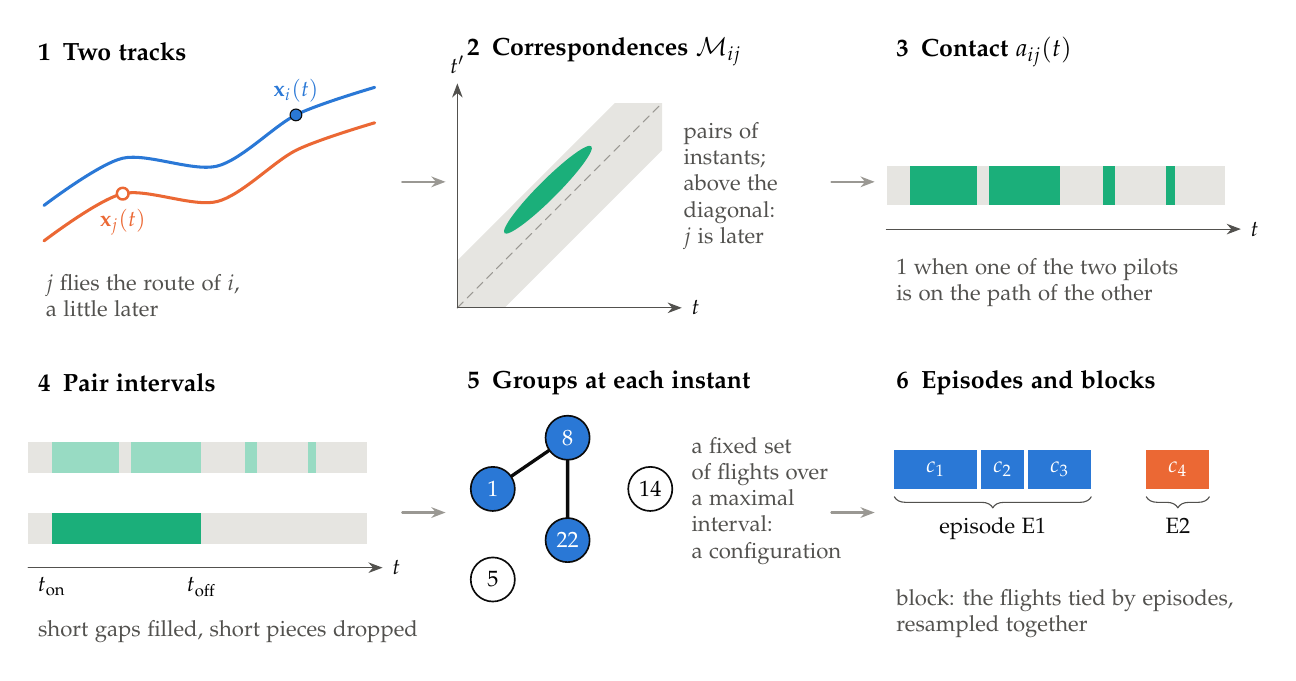
\begin{tikzpicture}[x=1cm,y=1cm]
  % 1: two tracks
  \begin{scope}[shift={(0,0)}]
    \node[panel] at (0,3.25) {1\enspace Two tracks};
    \draw[track i] plot[smooth] coordinates {(0.2,1.3) (1.2,1.9) (2.4,1.8) (3.4,2.45) (4.4,2.8)};
    \draw[track j] plot[smooth] coordinates {(0.2,0.85) (1.2,1.45) (2.4,1.35) (3.4,2.0) (4.4,2.35)};
    \node[pt i] (xi) at (3.4,2.45) {};
    \node[hollow j] (xj) at (1.2,1.45) {};
    \node[lbl, blueI, above=1pt] at (xi) {$\x_i(t)$};
    \node[lbl, orangeJ, below=2pt] at (xj) {$\x_j(t)$};
    \node[note, align=left, anchor=north west] at (0.1,0.55) {$j$ flies the route of $i$,\\a little later};
  \end{scope}
  % 2: correspondences
  \begin{scope}[shift={(5.45,0)}]
    \node[panel] at (0,3.25) {2\enspace Correspondences $\M_{ij}$};
    \fill[light] (0,0) -- (0.6,0) -- (2.6,2.0) -- (2.6,2.6) -- (2.0,2.6) -- (0,0.6) -- cycle;
    \draw[muted, densely dashed] (0,0) -- (2.6,2.6);
    \fill[aqua, rotate around={45:(1.15,1.5)}] (1.15,1.5) ellipse (0.78 and 0.12);
    \draw[->, ink2] (0,0) -- (2.85,0) node[right, lbl, ink] {$t$};
    \draw[->, ink2] (0,0) -- (0,2.85) node[above, lbl, ink] {$t'$};
    \node[note, align=left, anchor=west] at (2.75,1.55) {pairs of\\instants;\\above the\\diagonal:\\$j$ is later};
  \end{scope}
  % 3: contact
  \begin{scope}[shift={(10.9,0)}]
    \node[panel] at (0,3.25) {3\enspace Contact $a_{ij}(t)$};
    \draw[->, ink2] (0,1.0) -- (4.5,1.0) node[right, lbl, ink] {$t$};
    \fill[light] (0,1.3) rectangle (4.3,1.8);
    \foreach \a/\b in {0.3/1.15, 1.3/2.2, 2.75/2.9, 3.55/3.66} \fill[aqua] (\a,1.3) rectangle (\b,1.8);
    \node[note, align=left, anchor=north west] at (0,0.75) {$1$ when one of the two pilots\\is on the path of the other};
  \end{scope}
  % 4: pair intervals
  \begin{scope}[shift={(0,-4.2)}]
    \node[panel] at (0,3.25) {4\enspace Pair intervals};
    \fill[light] (0,2.1) rectangle (4.3,2.5);
    \foreach \a/\b in {0.3/1.15, 1.3/2.2, 2.75/2.9, 3.55/3.66} \fill[aqua!45] (\a,2.1) rectangle (\b,2.5);
    \fill[light] (0,1.2) rectangle (4.3,1.6);
    \fill[aqua] (0.3,1.2) rectangle (2.2,1.6);
    \draw[->, ink2] (0,0.9) -- (4.5,0.9) node[right, lbl, ink] {$t$};
    \node[lbl, below] at (0.3,0.9) {$t_{\rm on}$};
    \node[lbl, below] at (2.2,0.9) {$t_{\rm off}$};
    \node[note, align=left, anchor=north west] at (0,0.35) {short gaps filled, short pieces dropped};
  \end{scope}
  % 5: groups at each instant
  \begin{scope}[shift={(5.45,-4.2)}]
    \node[panel] at (0,3.25) {5\enspace Groups at each instant};
    \coordinate (n1) at (0.45,1.9); \coordinate (n8) at (1.4,2.55); \coordinate (n22) at (1.4,1.25);
    \coordinate (n14) at (2.45,1.9); \coordinate (n5) at (0.45,0.75);
    \draw[edge] (n1) -- (n8) -- (n22);
    \node[inE1] at (n1) {1}; \node[inE1] at (n8) {8}; \node[inE1] at (n22) {22};
    \node[flight] at (n14) {14}; \node[flight] at (n5) {5};
    \node[note, align=left, anchor=west] at (2.85,1.75) {a fixed set\\of flights over\\a maximal\\interval:\\a configuration};
  \end{scope}
  % 6: episodes and blocks
  \begin{scope}[shift={(10.9,-4.2)}]
    \node[panel] at (0,3.25) {6\enspace Episodes and blocks};
    \foreach \a/\b/\n in {0.1/1.15/1, 1.2/1.75/2, 1.8/2.6/3} {
      \fill[blueI] (\a,1.9) rectangle (\b,2.4);
      \node[font=\footnotesize, text=white] at ({(\a+\b)/2},2.15) {$c_\n$};
    }
    \fill[orangeJ] (3.3,1.9) rectangle (4.1,2.4);
    \node[font=\footnotesize, text=white] at (3.7,2.15) {$c_4$};
    \draw[decorate, decoration={brace, mirror, amplitude=4pt}, ink2] (0.1,1.8) -- (2.6,1.8)
      node[midway, below=4pt, lbl, ink] {episode E1};
    \draw[decorate, decoration={brace, mirror, amplitude=4pt}, ink2] (3.3,1.8) -- (4.1,1.8)
      node[midway, below=4pt, lbl, ink] {E2};
    \node[note, align=left, anchor=north west] at (0,0.75) {block: the flights tied by episodes,\\resampled together};
  \end{scope}
  % reading order
  \foreach \y in {1.6, -2.6} {
    \draw[->, muted, line width=0.8pt] (4.75,\y) -- (5.3,\y);
    \draw[->, muted, line width=0.8pt] (10.2,\y) -- (10.75,\y);
  }
\end{tikzpicture}
\caption{The method in six steps. Panels 1--3: the pair contact (Section~\ref{sec:contact}).
Panels 4--6: from pairs to groups (Section~\ref{sec:groups}). Flights 1, 8, 22, 14 and 5 are the
example day of Figure~\ref{fig:day}.}
\label{fig:overview}
\end{figure}

\begin{table}
\centering
\small
\begin{tabularx}{\textwidth}{@{}l X l l@{}}
\toprule
Object & In words & Symbol & Section \\
\midrule
Departure & the first fix farther than $R_\dep$ from the takeoff & $k_i^\dep$ & \ref{sec:local} \\
Correspondence & two instants, $t$ on the clock of $i$ and $t'$ on that of $j$, at most $\delta$ apart, at which the two pilots pass the same place within the tolerances & $(t,t')\in\M_{ij}$ & \ref{sec:correspondences} \\
Contact & at instant $t$, one of the two pilots is on the path of the other & $a_{ij}(t)=1$ & \ref{sec:correspondences} \\
Pair interval & a stretch of contact, with short gaps filled and short pieces dropped & $[t_{\rm on},t_{\rm off})$ & \ref{sec:pair-intervals} \\
Group at instant $t$ & the pilots joined to each other by chains of contacts at $t$ & component of $G(t)$ & \ref{sec:configurations} \\
Configuration & a fixed set of flights that stays one group over a maximal interval & $c$ & \ref{sec:configurations} \\
Membership & the label of flight $i$ at instant $t$: local phase, solo, or its configuration & $\gamma_i(t)$ & \ref{sec:configurations} \\
Episode & a chain of configurations, each starting when the previous one ends and sharing a member with it & & \ref{sec:episodes} \\
Dependency block & the flights tied together by episodes; the bootstrap resamples them together & & \ref{sec:blocks} \\
\bottomrule
\end{tabularx}
\caption{A minimal dictionary of the objects of the method.}
\label{tab:glossary}
\end{table}

\section{Motivation and requirements}\label{sec:motivation}

The statistical properties of free-flight trajectories (time spent in thermals, length of the
glides, mean squared displacement) are usually estimated by treating flights as independent
samples. The assumption fails when several pilots fly together: they share thermals and routes,
and their trajectories are correlated. Group flight may also change the behaviour itself. In
soaring birds, social information on the position of thermals changes the gliding
strategy~\cite{williams2018}, and in a migrating flock a few individuals find the thermals while
the others follow them~\cite{flack2018,nagy2018}. Comparing group flights with solo flights
therefore needs a rule that says, for every flight and every instant, whether the pilot is in a
group and with whom.

The intuitive notion of \emph{flying together} that the rule must make operational is the
following (Figure~\ref{fig:requirements}).
\begin{enumerate}[label=(R\arabic*), leftmargin=3.2em]
  \item The pilots take off from the same area, not necessarily from the same takeoff.
  \item Departures may be staggered, but not to the point of losing sight of each other.
  \item The pilots follow roughly the same route: nearby places and similar motion, not
        necessarily the same points.
  \item The composition of the group changes in time: some pilots join, others change route.
\end{enumerate}

\begin{figure}
\centering
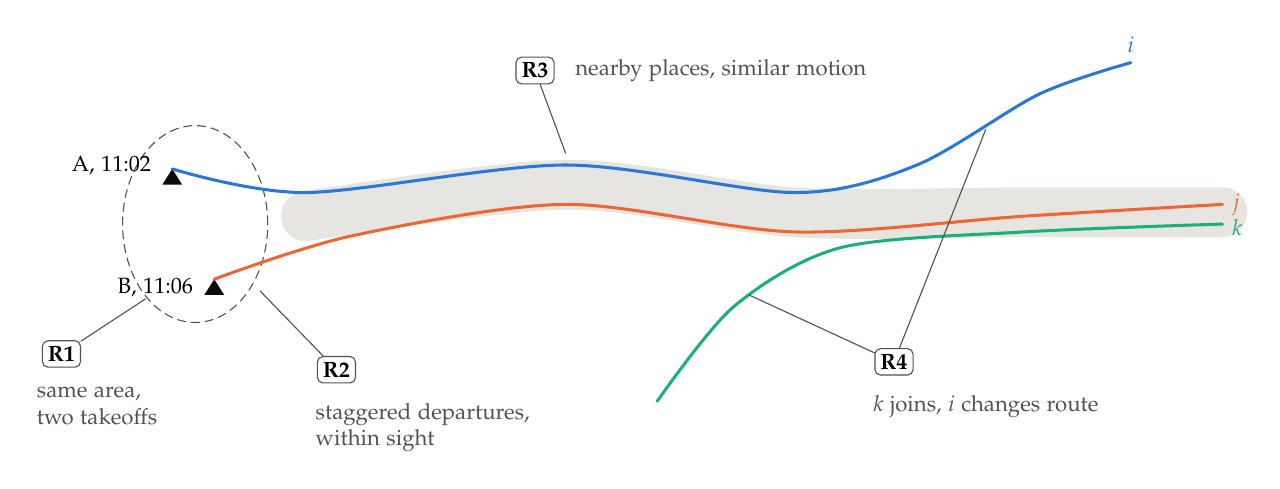
\begin{tikzpicture}[x=0.97cm,y=1cm,
    tag/.style={draw=ink2, rounded corners=2pt, fill=white, font=\footnotesize\bfseries, inner sep=2pt}]
  \draw[light, line width=18pt, line cap=round] plot[smooth] coordinates {(2.6,2.35) (6,2.75) (9,2.4) (12,2.4) (14.6,2.4)};
  \draw[ink2, densely dashed] (1.15,2.25) ellipse (0.95 and 1.25);
  \fill[ink] (0.85,2.95) -- ++(-0.13,-0.2) -- ++(0.26,0) -- cycle;
  \fill[ink] (1.4,1.55) -- ++(-0.13,-0.2) -- ++(0.26,0) -- cycle;
  \node[lbl, left] at (0.7,3.0) {A, 11:02};
  \node[lbl, left] at (1.25,1.45) {B, 11:06};
  \draw[track i] plot[smooth] coordinates {(0.85,2.95) (2.6,2.65) (6,3.0) (9,2.65) (10.6,3.0) (12.2,3.9) (13.4,4.3)};
  \draw[track j] plot[smooth] coordinates {(1.4,1.55) (3.2,2.1) (6,2.5) (9,2.15) (12,2.35) (14.6,2.5)};
  \draw[track k] plot[smooth] coordinates {(7.2,0.0) (8.2,1.2) (9.6,1.95) (12,2.15) (14.6,2.25)};
  \node[lbl, blueI, above] at (13.4,4.3) {$i$};
  \node[lbl, orangeJ, right] at (14.6,2.5) {$j$};
  \node[lbl, aqua, right] at (14.6,2.2) {$k$};
  \node[tag] (r1) at (-0.6,0.6) {R1};
  \draw[ink2] (r1) -- (0.5,1.3);
  \node[note, align=left, anchor=north west] at (-1.05,0.3) {same area,\\two takeoffs};
  \node[tag] (r2) at (3.0,0.4) {R2};
  \draw[ink2] (r2) -- (2.0,1.4);
  \node[note, align=left, anchor=north west] at (2.6,0.1) {staggered departures,\\within sight};
  \node[tag] (r3) at (5.6,4.2) {R3};
  \draw[ink2] (r3) -- (6.0,3.15);
  \node[note, align=left, anchor=west] at (6.0,4.2) {nearby places, similar motion};
  \node[tag] (r4) at (10.3,0.5) {R4};
  \draw[ink2] (r4) -- (8.4,1.35);
  \draw[ink2] (r4) -- (11.5,3.45);
  \node[note, align=left, anchor=north west] at (9.9,0.2) {$k$ joins, $i$ changes route};
\end{tikzpicture}
\caption{The four requirements on a schematic map. Pilots $i$ and $j$ take off from two places of
the same area four minutes apart and follow the same corridor (grey) without flying over the same
points; $k$ joins later and $i$ leaves the corridor.}
\label{fig:requirements}
\end{figure}

Three immediate approaches do not meet these requirements (Figure~\ref{fig:approaches}).
\begin{itemize}
  \item \textbf{Geometric similarity of the tracks} (Hausdorff, Fréchet, unconstrained DTW;
    survey in~\cite{su2020}). Cross-country routes are channelled by the terrain and thermals
    are often anchored to the ground: two independent pilots who took off from the same site
    produce similar tracks even hours apart. Unconstrained DTW, moreover, warps the time axis
    without limit and erases exactly the information that (R2) needs.
  \item \textbf{Strict synchrony} (flock~\cite{gudmundsson2006}, convoy~\cite{jeung2008},
    swarm~\cite{li2010}). These patterns require proximity at the same instant; the swarm
    admits non-consecutive instants but no delay between members. Two pilots on the same route
    two minutes apart are never close at the same instant, yet they fly together in the sense
    of (R2)--(R3).
  \item \textbf{Window on the departures.} A rule such as ``departures within $T$ minutes''
    produces groups that depend on the reference pilot: if 1 and 8 depart within the window,
    and so do 8 and 14, then 1 and 14 need not (Section~\ref{sec:transitivity}).
\end{itemize}

\begin{figure}
\centering
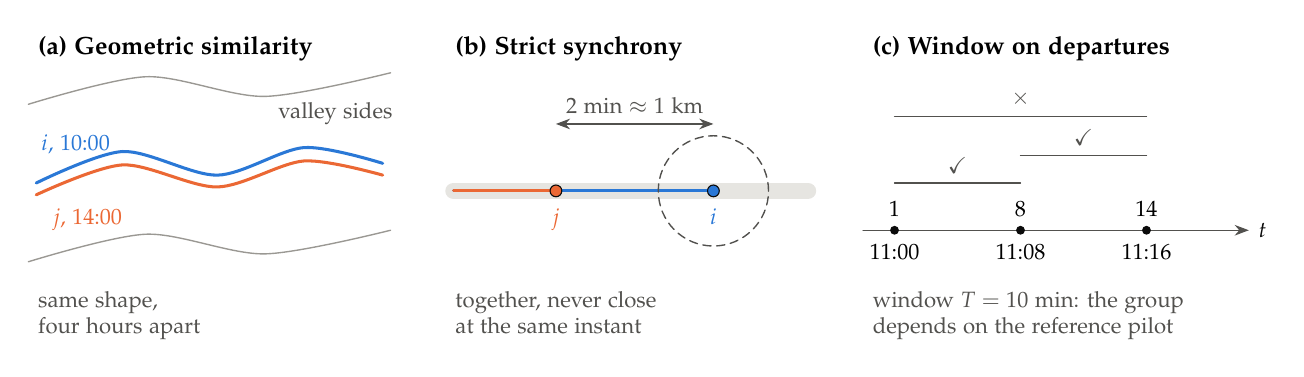
\begin{tikzpicture}[x=1cm,y=1cm]
  % (a) geometric similarity
  \begin{scope}[shift={(0,0)}]
    \node[panel] at (0,3.3) {(a) Geometric similarity};
    \draw[muted, line width=0.5pt] plot[smooth] coordinates {(0,2.6) (1.5,2.95) (3,2.7) (4.6,3.0)};
    \draw[muted, line width=0.5pt] plot[smooth] coordinates {(0,0.6) (1.5,0.95) (3,0.7) (4.6,1.0)};
    \node[note, anchor=north] at (3.9,2.75) {valley sides};
    \draw[track i] plot[smooth] coordinates {(0.1,1.6) (1.2,2.0) (2.4,1.7) (3.5,2.05) (4.5,1.85)};
    \draw[track j] plot[smooth] coordinates {(0.1,1.45) (1.2,1.83) (2.4,1.55) (3.5,1.88) (4.5,1.7)};
    \node[lbl, blueI, above] at (0.6,1.85) {$i$, 10:00};
    \node[lbl, orangeJ, below] at (0.75,1.4) {$j$, 14:00};
    \node[note, align=left, anchor=north west] at (0,0.35) {same shape,\\four hours apart};
  \end{scope}
  % (b) strict synchrony
  \begin{scope}[shift={(5.3,0)}]
    \node[panel] at (0,3.3) {(b) Strict synchrony};
    \draw[light, line width=6pt] (0.1,1.5) -- (4.6,1.5);
    \draw[track i] (0.1,1.5) -- (3.4,1.5);
    \draw[track j] (0.1,1.5) -- (1.4,1.5);
    \node[pt i] at (3.4,1.5) {};
    \node[pt j] at (1.4,1.5) {};
    \draw[tol] (3.4,1.5) circle (0.7);
    \draw[<->, ink2] (1.4,2.35) -- node[above, lbl] {2 min $\approx$ 1 km} (3.4,2.35);
    \node[lbl, orangeJ, below=3pt] at (1.4,1.5) {$j$};
    \node[lbl, blueI, below=3pt] at (3.4,1.5) {$i$};
    \node[note, align=left, anchor=north west] at (0,0.35) {together, never close\\at the same instant};
  \end{scope}
  % (c) window on departures
  \begin{scope}[shift={(10.6,0)}]
    \node[panel] at (0,3.3) {(c) Window on departures};
    \draw[->, ink2] (0,1.0) -- (4.9,1.0) node[right, lbl, ink] {$t$};
    \foreach \x/\f/\h in {0.4/1/11:00, 2.0/8/11:08, 3.6/14/11:16} {
      \fill[ink] (\x,1.0) circle (1.6pt);
      \node[lbl, below] at (\x,0.95) {\h};
      \node[lbl, above] at (\x,1.05) {\f};
    }
    \draw[ink2] (0.4,1.6) -- (2.0,1.6) node[midway, above, lbl] {\checkmark};
    \draw[ink2] (2.0,1.95) -- (3.6,1.95) node[midway, above, lbl] {\checkmark};
    \draw[ink2] (0.4,2.45) -- (3.6,2.45) node[midway, above, lbl] {$\times$};
    \node[note, align=left, anchor=north west] at (0,0.35) {window $T = 10$ min: the group\\depends on the reference pilot};
  \end{scope}
\end{tikzpicture}
\caption{Why three immediate rules fail. (a) Two independent pilots on the same valley produce
similar tracks hours apart. (b) Two pilots on the same route two minutes apart never enter each
other's proximity disc. (c) With a window of 10 minutes, 1--8 and 8--14 pass and 1--14 fails.}
\label{fig:approaches}
\end{figure}

\section{Relation to the literature}\label{sec:literature}

This section says where each ingredient of the method comes from and what, as far as a targeted
but not exhaustive search shows, has not been done yet.

\subsection{Trajectory similarity with a temporal tolerance}

The LCSS of Vlachos, Kollios and Gunopulos~\cite{vlachos2002} matches two points when they are
closer than $\varepsilon$ in every coordinate and their \emph{indices} in the two sequences differ
by at most $\delta$. The similarity $S_1$ is the length of the common subsequence divided by the
length of the shorter track, and the variant $S_2$ maximises $S_1$ over all spatial translations,
to recognise parallel movements. The EDR of Chen, Özsu and Oria~\cite{chen2005} and DTW with a
Sakoe--Chiba band~\cite{sakoe1978} bound the shift in the same way. These measures return a
single number per pair of tracks: they say how similar two tracks are, and not \emph{when} two
pilots are together. A bound on indices counted from the first point of each track also mixes
the shift between the takeoffs with the delay in flight, and $S_2$ matches precisely the parallel
routes that we want to exclude.

The measures of joint movement that do say when are built on simultaneous fixes. The proximity
index Prox is the share of simultaneous fixes closer than a threshold~\cite[§3.1]{joo2018}: with
$\delta=0$ and without the conditions on height and heading, it is the share of the flight of $i$
in contact with $j$ in the sense of Section~\ref{sec:correspondences}.

\subsection{Following with a delay}\label{sec:following}

The closest precedent of our pair contact is the following of Li, Wu and Crofoot~\cite{li2013},
defined on tracks sampled at the same instants (Figure~\ref{fig:li}). At instant $i$ the local
lag $\Delta(i)$ is the shift $t$, with $|t|\le l_{\max}$, that minimises the distance between the
position $r_i$ of $R$ and the position $s_{i-t}$ of $S$. The instant is \emph{valid} if this
minimum distance is below $d_{\max}$, and $R$ follows $S$ at a valid instant if $\Delta(i)>0$
(§IV-A). The lag is therefore local and free to vary, and its sign separates the follower from
the leader. Two individuals that merely move together lead and follow equally often, so the
following intervals are the stretches with more following instants than the half expected
without following: the maximal segments of $f(i)-1/2$, with $f(i)=1$ when $R$ follows and $0$
otherwise, found in linear time~\cite{ruzzo1999} (§IV-B) and checked with the roles
reversed (§IV-C). The threshold $d_{\max}$ only discards the instants without interaction, and
does not move the minimiser.

Our contact keeps the window of lags and the distance threshold, and leaves the sign out: the
contact of $i$ with $j$ at instant $t$ is the validity of $t$, with tolerances on height and
heading added (Section~\ref{sec:correspondences}). We want the pairs that fly together, whether
or not one of them leads; who follows whom comes back afterwards, through the median lag of each
contact (Section~\ref{sec:phase3}).

\begin{figure}
\centering
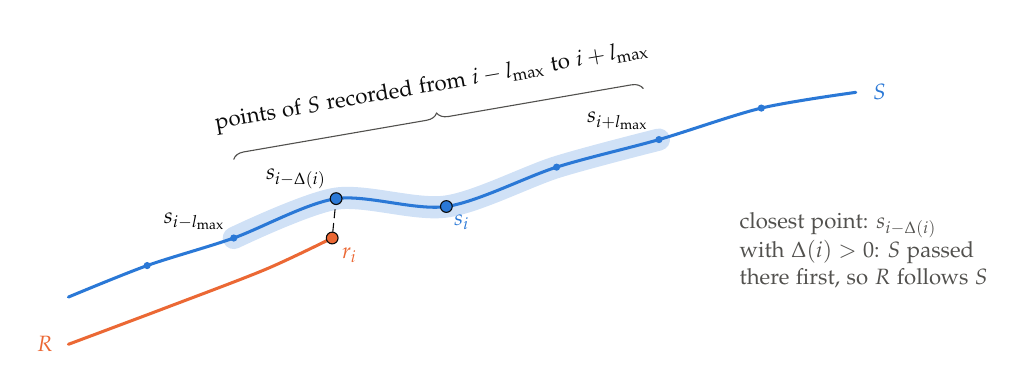
\begin{tikzpicture}[x=1cm,y=1cm]
  \draw[track i, line width=8pt, blueI!22] plot[smooth] coordinates {(2.1,1.35) (3.4,1.85) (4.8,1.75) (6.2,2.25) (7.5,2.6)};
  \draw[track i] plot[smooth] coordinates {(0,0.6) (1.0,1.0) (2.1,1.35) (3.4,1.85) (4.8,1.75) (6.2,2.25) (7.5,2.6) (8.8,3.0) (10,3.2)};
  \foreach \p in {(1.0,1.0),(2.1,1.35),(3.4,1.85),(4.8,1.75),(6.2,2.25),(7.5,2.6),(8.8,3.0)} \fill[blueI] \p circle (1.3pt);
  \node[lbl, above left=-1pt] at (2.1,1.35) {$s_{i-l_{\max}}$};
  \node[lbl, above left] at (7.5,2.6) {$s_{i+l_{\max}}$};
  \node[pt i] (si) at (4.8,1.75) {};
  \node[lbl, blueI, below right=-1pt] at (si) {$s_i$};
  \draw[track j] plot[smooth] coordinates {(0,0.0) (1.2,0.45) (2.5,0.95) (3.35,1.35)};
  \node[pt j] (ri) at (3.35,1.35) {};
  \node[lbl, orangeJ, below right] at (ri) {$r_i$};
  \node[pt i] (sd) at (3.4,1.85) {};
  \draw[ink, densely dashed] (ri) -- (sd);
  \node[lbl, above left] at (sd) {$s_{i-\Delta(i)}$};
  \node[lbl, blueI] at (10.3,3.2) {$S$};
  \node[lbl, orangeJ] at (-0.3,0.0) {$R$};
  \draw[decorate, decoration={brace, amplitude=4pt}, ink2] (2.1,2.35) -- (7.3,3.25)
    node[midway, above=6pt, lbl, ink, sloped] {points of $S$ recorded from $i-l_{\max}$ to $i+l_{\max}$};
  \node[note, align=left, anchor=west] at (8.4,1.2) {closest point: $s_{i-\Delta(i)}$\\with $\Delta(i)>0$: $S$ passed\\there first, so $R$ follows $S$};
\end{tikzpicture}
\caption{Following with a local lag~\cite{li2013}. At instant $i$, the track of $S$ is searched
in the time window $[i-l_{\max}, i+l_{\max}]$ (shaded) for the point closest to the position
$r_i$ of $R$. The best lag $\Delta(i)$ is positive: $R$ is now where $S$ was $\Delta(i)$
earlier.}
\label{fig:li}
\end{figure}

Nagy et al.~\cite{nagy2010} measure the delay between two pigeons as the shift that maximises the
correlation of their headings, and build leader--follower hierarchies from its sign. In a thermal
the heading turns through $2\pi$ every 20--30~s, so this correlation, like the distance of
Section~\ref{sec:roles}, repeats with the period of the turn. Konzack et al.~\cite{konzack2017}
display such local delays between simultaneously recorded tracks in a ``delay space'', comparing
Fréchet, DTW and edit-distance matchings. FLICA and its package
mFLICA~\cite{amornbunchornvej2018a,amornbunchornvej2018b,amornbunchornvej2021} infer a following
network in sliding time windows, with DTW restricted to a Sakoe--Chiba band, and call the faction
of a leader the individuals that reach it through a directed path: groups built from delayed
following, but directed, with leaders, and on windows. The following of Andersson et
al.~\cite{andersson2007} is instantaneous: an individual follows another that is in a sector
ahead of it with a similar heading.

\subsection{Group structure in time}

Buchin et al.~\cite{buchin2015} call two entities directly connected at time $t$ if their
$\varepsilon$-discs overlap, and $\varepsilon$-connected if a chain of direct connections joins
them at that instant; the maximal $\varepsilon$-connected sets, the components, partition the
entities at every instant. The Reeb graph records how the components evolve: its vertices are the
events (start, end, merge, split), and each edge is a fixed set of entities that forms one
component over an interval of time (Figure~\ref{fig:reeb}). On it they define the maximal groups,
sets of at least $m$ entities that stay inside one component for at least a duration $\delta$;
maximal groups may overlap, and an entity can belong to several at once. Two more ideas of theirs
reappear below: a robust structure ignores interruptions shorter than $\alpha$, by calling two
entities connected at $t$ when they were directly connected at some instant within $\alpha/2$ of
$t$ (§4); and the grouping structure can split the trajectories into independent data sets
(§1). The proximity is always simultaneous.

\begin{figure}
\centering
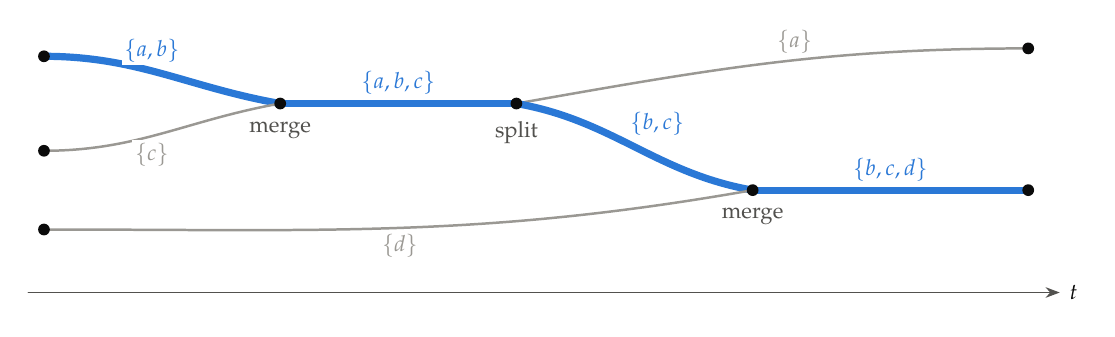
\begin{tikzpicture}[x=1cm,y=1cm,
    vtx/.style={circle, fill=ink, inner sep=1.5pt},
    single/.style={muted, line width=0.9pt},
    multi/.style={blueI, line width=2.6pt},
    set/.style={font=\footnotesize, fill=white, inner sep=1pt}]
  \coordinate (s1) at (0,2.2); \coordinate (s2) at (0,1.0); \coordinate (s3) at (0,0.0);
  \coordinate (m1) at (3.0,1.6); \coordinate (sp) at (6.0,1.6); \coordinate (m2) at (9.0,0.5);
  \coordinate (e1) at (12.5,2.3); \coordinate (e2) at (12.5,0.5);
  \draw[multi] (s1) to[out=0, in=170] node[set, pos=0.45, above=1pt] {$\{a,b\}$} (m1);
  \draw[single] (s2) to[out=0, in=190] node[set, pos=0.45, below=1pt] {$\{c\}$} (m1);
  \draw[multi] (m1) -- node[set, above=1pt] {$\{a,b,c\}$} (sp);
  \draw[single] (sp) to[out=10, in=180] node[set, pos=0.55, above=1pt] {$\{a\}$} (e1);
  \draw[multi] (sp) to[out=-10, in=170] node[set, pos=0.45, above right=0pt] {$\{b,c\}$} (m2);
  \draw[single] (s3) to[out=0, in=190] node[set, pos=0.5, below=1pt] {$\{d\}$} (m2);
  \draw[multi] (m2) -- node[set, above=1pt] {$\{b,c,d\}$} (e2);
  \foreach \v in {s1,s2,s3,m1,sp,m2,e1,e2} \node[vtx] at (\v) {};
  \node[note, below=3pt] at (m1) {merge};
  \node[note, below=3pt] at (sp) {split};
  \node[note, below=3pt] at (m2) {merge};
  \draw[->, ink2] (-0.2,-0.8) -- (12.9,-0.8) node[right, lbl, ink] {$t$};
\end{tikzpicture}
\caption{The grouping structure of Buchin et al.~\cite{buchin2015} as a Reeb graph. Each edge is a
fixed set of entities that forms one connected component over an interval; vertices are starts,
ends, merges and splits. The thick edges have at least two entities: in this note they become the
configurations (Section~\ref{sec:configurations}), built on delayed contacts.}
\label{fig:reeb}
\end{figure}

\subsection{Interaction indices and null models}

Joo et al.~\cite{joo2018} sort the metrics of joint movement between pairs by what they capture,
proximity or coordination. Long et al.~\cite{long2014} compare eight of them on simulated tracks
and on deer: the indices that rest on a statistical test report interactions that are not there,
more often the finer the sampling, and the indices that return one number per pair miss the
interactions that come and go; the wildlifeDI package~\cite{long2022} extends the analysis to
contacts in high-frequency data. Spiegel et al.~\cite{spiegel2016} build a null model by shuffling
whole days of each individual's path among its days: each individual keeps its use of space, and
the synchrony between individuals is lost.

\subsection{Collective soaring}

Ákos, Nagy and Vicsek~\cite{akos2008} compare the soaring of birds with that of paraglider and
hang-glider pilots on GPS tracks; falcons, storks and paragliders circle with radii of 20--26~m.
In migrating white storks a few leaders find and explore the thermals and the others follow them,
leaving the thermals earlier and lower~\cite{flack2018}; inside a thermal, flock mates
synchronise their circling~\cite{nagy2018}. Vultures informed by other birds of the next updraft
glide towards it faster~\cite{williams2018}. We found no work that identifies group flights
systematically in large free-flight datasets.

\subsection{What we take and what is new}

The method is not a new general algorithm for grouping trajectories. The pair contact is the
proximity with a local lag of Li et al.~\cite{li2013}, the group structure is that of Buchin et
al.~\cite{buchin2015}, and groups built from delayed relations exist in
mFLICA~\cite{amornbunchornvej2021}, with other definitions (Table~\ref{tab:origin}). What we did
not find in the literature is:
\begin{enumerate}[label=(\roman*)]
  \item the Reeb structure built on contacts with a local delay instead of simultaneous proximity;
  \item the adaptations to thermal flight: a vertical tolerance that separates pilots circling in
        the same thermal at distant heights, and headings compared only in glide
        (Section~\ref{sec:roles});
  \item the application to a free-flight dataset of this size, with thresholds calibrated on a
        null model.
\end{enumerate}
The contribution is therefore a physically motivated adaptation and a scalable implementation,
more than a new method in itself, and the thesis should present it in these terms.

\begin{table}
\centering
\small
\begin{tabularx}{\textwidth}{@{}>{\raggedright}p{2.1cm} >{\raggedright}p{2.6cm} >{\raggedright}X >{\raggedright\arraybackslash}X@{}}
\toprule
Component & Precedent & What we take & What we change \\
\midrule
Pair contact with a delay & Li et al.~\cite{li2013}; tolerance in~\cite{vlachos2002,chen2005,sakoe1978} &
  window of lags and distance threshold; local lag, free to vary &
  height tolerance (separates heights within a thermal); heading only in glide; local phase
  excluded; no sign in the contact, $a_{ij}=a_{ji}$ (the sign returns in $\ell_{\rm med}$) \\ \addlinespace
Contact intervals & robustness in~\cite{buchin2015}; maximal segments in~\cite{li2013} &
  tolerance to short interruptions &
  gaps shorter than $g$ filled; minimum duration calibrated on a null model \\ \addlinespace
Groups in time & Buchin et al.~\cite{buchin2015} & components and their Reeb graph; configurations
  are its edges with at least two entities &
  built on delayed contacts; episodes are the connected parts of the Reeb graph without single
  entities; no maximal groups \\ \addlinespace
Groups from following & mFLICA~\cite{amornbunchornvej2021} & -- &
  undirected groups without leaders; exact intervals instead of sliding windows \\ \addlinespace
Null model & Spiegel et al.~\cite{spiegel2016}; SAM~\cite{tusher2001} & time shift of the tracks;
  false discovery rate as chance count over observed count &
  shift within the day, drawn from the real delays between takeoffs; chance count per unit of
  exposure \\ \addlinespace
Computation & filter--refine scheme & -- &
  no-loss lemma for delayed contacts; KD-tree with a time coordinate \\
\bottomrule
\end{tabularx}
\caption{Where the ingredients of the method come from.}
\label{tab:origin}
\end{table}

\paragraph{Essential reading.} The two readings to do first are Li et al.~\cite{li2013},
Sections~II and~IV (following, local lag, score), and Buchin et al.~\cite{buchin2015}, Sections~1,
2.1 and~4 of the arXiv version (groups, Reeb graph, robustness). Long et al.~\cite{long2014} and
Spiegel et al.~\cite{spiegel2016} serve the null model; Vlachos et al.~\cite{vlachos2002} and Joo
et al.~\cite{joo2018} place the measures of similarity and proximity.

\section{Data and notation}\label{sec:data}

The flights are those of the xc-dynamics pre-processing. Each flight $i\in V$ is one or more
segments of fixes, from its takeoff $k^0_i$ to its landing $k^\fin_i$ (step~8 of the
pre-processing, take-off and landing); between two segments the track has a gap. A fix has a
time, a latitude $\varphi$, a longitude $\lambda$ and the GNSS altitude $z$, at the interval of
its logger: one second for 70\% of the paraglider flights, two to ten seconds for most of the
others. Time $k$ is in UTC seconds from the start of the day, on the same clock for all flights;
IGC times are whole seconds.

Positions follow the frame of the thesis (chapter Trajectory pre-processing, section Local
coordinates and vertical datum): each fix is moved to the point of the WGS84 ellipsoid below it,
$h=0$, and converted to Earth-centred Cartesian coordinates, $\x_i(k)\in\R^3$. The thesis then
rotates them into the east and north of the first fix of each flight; here they stay
Earth-centred, so the coordinates of all flights are the same frame. The distance between two
positions is the chord of the ellipsoid, shorter than the distance along it by about $d^3/24R^2$:
about a millimetre at $d=10$~km. The altitude is $z$ as recorded.

The phase labelling of xc-lab (note \emph{Flight phases with a hidden Markov model}) gives every
fix of a flight logged every 5~s or less one of three states,
$s_i(k)\in\{\st{climb}, \st{search}, \st{transition}\}$: climbing in a thermal, searching for the
next one, gliding between two thermals. In the text \emph{glide} means the state
\st{transition}. The fixes of coarser loggers and of pieces too short to be labelled stay
unclassified.

\begin{table}
\centering
\small
\begin{tabularx}{\textwidth}{@{}l >{\raggedright\arraybackslash}X l l@{}}
\toprule
Symbol & Meaning & Start & Chosen \\
\midrule
$\x_i(k)\in\R^3$ & position: the point of the ellipsoid below the fix, Earth-centred & & \\
$z_i(k)$ & GNSS altitude & & \\
$s_i(k)$ & state: \st{climb}, \st{search}, \st{transition} (glide), or unclassified & & \\
$\vh_i(k)$ & horizontal heading, used only in glide & & \\
$k^0_i,\ k^\fin_i,\ k^\dep_i$ & takeoff, landing, departure (Section~\ref{sec:local}) & & \\
$T^\dep_i$ & the grid instants from departure to landing at which flight $i$ has a position & & \\
$R_\dep$ & radius of the local phase around the takeoff & 3 km & 3 km \\
$\Delta$ & step of the common time grid $\Delta\Z$ & 5 s & 5 s \\
$h_{\max}$ & longest time between two fixes across which a grid position is interpolated & 10 s & 10 s \\
$\delta$ & maximum delay between two pilots, always a time & 5 min & 2 min \\
$\varepsilon_h,\ \varepsilon_z$ & horizontal and vertical tolerances & 500 m, 300 m & 500 m, 300 m \\
$\theta_{\max}$ & maximum angle between the headings in glide & 45\textdegree & 45\textdegree \\
$g$ & longest gap filled in a contact & 120 s & 120 s \\
$\tau^*$ & minimum duration of a contact & from the null model & 38.1 min \\
$v_\xc$ & mean cross-country speed, measured on the data & $\approx5$ m/s & \\
$v_{\max}$ & top speed between two fixes, set by the pre-processing (\texttt{speed.max\_kmh}) & 100 km/h & 100 km/h \\
$\varepsilon_\vis$ & visual range & 1.5 km & \\
$r_{\min},\ R_s$ & smallest time shift and radius of the takeoffs in the null model & $>2\delta$, 10 km & $2\delta+\Delta$, 10 km \\
$q$ & false discovery rate accepted for the contacts & 0.05 & 0.1 \\
\bottomrule
\end{tabularx}
\caption{Symbols and parameters, with their starting values and the values chosen on the data
(Section~\ref{sec:tuning}). Beware: in~\cite{vlachos2002}
$\delta$ is a tolerance on indices, in~\cite{joo2018} a distance threshold, in~\cite{buchin2015}
a minimum duration; here it is always a delay.}
\label{tab:notation}
\end{table}

\section{The pair contact}\label{sec:contact}

\subsection{Local phase}\label{sec:local}

Near the takeoff every pilot is close to every other, ridge soaring or waiting for the thermals,
and a contact in this phase says nothing about (R3). The departure is the first fix farther than
$R_\dep$ from the takeoff:
\begin{equation}\label{eq:departure}
  k^\dep_i = \min\bigl\{k:\ \|\x_i(k)-\x_i(k^0_i)\| > R_\dep\bigr\}.
\end{equation}
From then on the flight is evaluated on $T^\dep_i$, the instants of the common grid, one every
$\Delta$ seconds, from the departure to the landing at which the flight has a position
(Section~\ref{sec:phase0}). The instants before the departure are not evaluated, and a flight
that never leaves the disc is \emph{local}. Both get the state \st{L} and do not count as solo
flight (Figure~\ref{fig:local}).

\begin{figure}
\centering
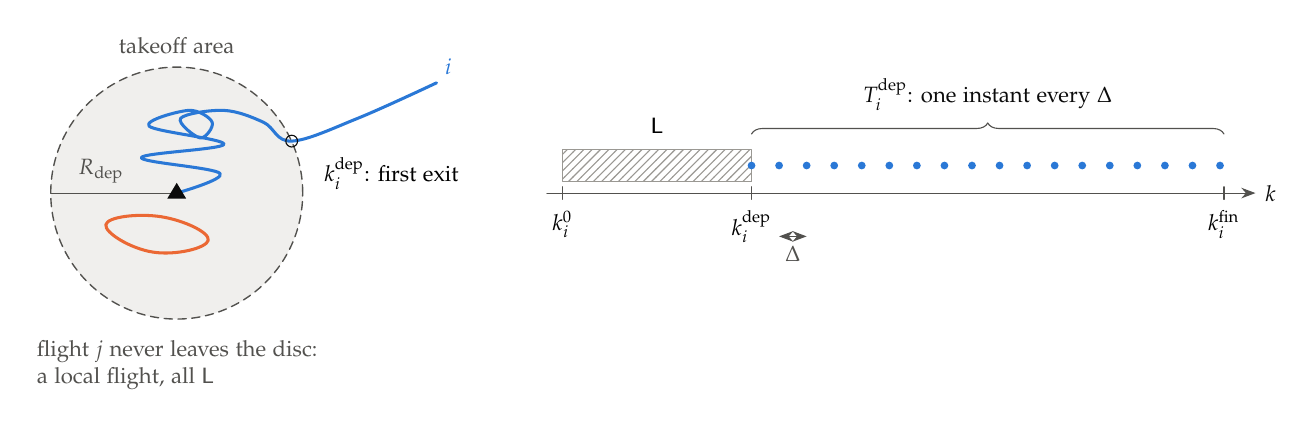
\begin{tikzpicture}[x=1cm,y=1cm]
  \begin{scope}
    \fill[light!60] (0,0) circle (1.6);
    \draw[tol] (0,0) circle (1.6);
    \draw[ink2] (0,0) -- (-1.6,0) node[pos=0.6, above, lbl] {$R_\dep$};
    \draw[track i] plot[smooth, tension=0.6] coordinates {(0,0) (0.55,0.25) (-0.45,0.45) (0.6,0.62)
      (-0.35,0.85) (0.15,1.05) (0.45,0.9) (0.3,0.7) (0.05,0.95) (0.6,1.05) (1.1,0.9) (1.46,0.66) (2.3,0.95) (3.3,1.4)};
    \draw[track j] plot[smooth cycle, tension=0.8] coordinates {(-0.9,-0.4) (-0.3,-0.75) (0.4,-0.6) (-0.2,-0.3)};
    \fill[ink] (0,0.13) -- ++(-0.12,-0.2) -- ++(0.24,0) -- cycle;
    \node[pt] (ex) at (1.46,0.66) {};
    \node[lbl, anchor=west, align=left] at (1.75,0.25) {$k^\dep_i$: first exit};
    \node[note, anchor=north west, align=left] at (-1.9,-1.75) {flight $j$ never leaves the disc:\\a local flight, all \st{L}};
    \node[lbl, blueI] at (3.45,1.6) {$i$};
    \node[note, anchor=south] at (0,1.65) {takeoff area};
  \end{scope}
  \begin{scope}[shift={(4.7,0)}]
    \draw[->, ink2] (0,0) -- (9.0,0) node[right, lbl, ink] {$k$};
    \fill[pattern=north east lines, pattern color=muted] (0.2,0.15) rectangle (2.6,0.55);
    \draw[muted] (0.2,0.15) rectangle (2.6,0.55);
    \node[lbl] at (1.4,0.85) {\st{L}};
    \foreach \x in {2.6,2.95,...,8.6} \fill[blueI] (\x,0.35) circle (1.4pt);
    \draw[ink2] (0.2,-0.08) -- (0.2,0.08); \node[lbl, below] at (0.2,-0.1) {$k^0_i$};
    \draw[ink2] (2.6,-0.08) -- (2.6,0.08); \node[lbl, below] at (2.6,-0.1) {$k^\dep_i$};
    \draw[ink2] (8.6,-0.08) -- (8.6,0.08); \node[lbl, below] at (8.6,-0.1) {$k^\fin_i$};
    \draw[decorate, decoration={brace, amplitude=4pt}, ink2] (2.6,0.75) -- (8.6,0.75)
      node[midway, above=5pt, lbl, ink] {$T^\dep_i$: one instant every $\Delta$};
    \draw[<->, ink2] (2.95,-0.55) -- (3.3,-0.55) node[midway, below, lbl] {$\Delta$};
  \end{scope}
\end{tikzpicture}
\caption{Local phase. Left: near the takeoff the pilot ridge soars and circles inside the disc of
radius $R_\dep$; the departure $k^\dep_i$ is the first fix outside it. A flight that never leaves
the disc is local. Right: the same flight in time; before the departure the state is \st{L}, after
it the flight is evaluated on the grid instants $T^\dep_i$.}
\label{fig:local}
\end{figure}

\subsection{Correspondences and contact}\label{sec:correspondences}

\begin{definition}[correspondence]\label{def:correspondence}
For two flights $i\ne j$, the set of correspondences is
\begin{equation}\label{eq:correspondences}
  \begin{split}
  \M_{ij} = \Bigl\{(t,t')\in T^\dep_i\times T^\dep_j:\ & |t'-t|\le\delta,\ \ \|\x_i(t)-\x_j(t')\|<\varepsilon_h,\\
  & |z_i(t)-z_j(t')|<\varepsilon_z,\ \ D_{ij}(t,t')=1\Bigr\},
  \end{split}
\end{equation}
where the heading condition is active only when both pilots glide:
\begin{equation}\label{eq:heading}
  D_{ij}(t,t') = \begin{cases}
    \ind\bigl[\vh_i(t)\cdot\vh_j(t') > \cos\theta_{\max}\bigr] & \text{if } s_i(t)=s_j(t')=\st{transition},\\
    1 & \text{otherwise.}
  \end{cases}
\end{equation}
\end{definition}

\begin{inwords}
$\M_{ij}$ is a set of \emph{pairs of instants}. The pair $(t,t')$ belongs to it when $j$, at its
instant $t'$, is where $i$ is at its instant $t$: within $\varepsilon_h$ horizontally and
$\varepsilon_z$ vertically, with the two instants at most $\delta$ apart, and heading the same way
if both glide. In the $(t,t')$ plane of Figure~\ref{fig:contact} it is a region inside the band
$|t'-t|\le\delta$.
\end{inwords}

\begin{figure}
\centering
\animated{contact}
\caption{\animmark Correspondences and contact for a synthetic pair; the animation runs the
instant $t$ from 0 to 1200~s. Left: plan view around $i$ at $t=420$~s. Pilot $j$ flies the route of $i$ 120~s later and 250~m to
the side; the circle has radius $\varepsilon_h$; the orange band is the part of the track of $j$
flown between $t-\delta$ and $t+\delta$; the dark dots are the instants $t'$ with
$(t,t')\in\M_{ij}$, and the segment joins $\x_i(t)$ to the closest of them, at delay $l=+120$~s.
At the same instant $j$ is about 1~km away: there is no simultaneous proximity. Top right: $\M_{ij}$
(green) in the $(t,t')$ plane, inside the band $|t'-t|\le\delta$ (grey); the black segment is the
column of the instant of the left panel. $\M_{ij}$ lies above the diagonal because $j$ passes
later. Bottom right: $m_{ij}$ projects $\M_{ij}$ on the $t$ axis, $m_{ji}$ on the $t'$ axis, and
$a_{ij}$ is their union: $i$ is on the path of $j$ from 90 to 775~s, $j$ on the path of $i$ from
220 to 885~s. Model: $i$ flies at 8~m/s along $y=600\sin(2\pi s/8\,\mathrm{km})$~m, where $s$ is
the distance flown; $j$ joins the route at 300~s and leaves it at 800~s, drifting sideways at
3~m/s; altitude and heading conditions hold throughout.}
\label{fig:contact}
\end{figure}

\begin{definition}[contact]\label{def:contact}
\begin{equation}\label{eq:contact}
  m_{ij}(t) = \ind\bigl[\exists\, t':\ (t,t')\in\M_{ij}\bigr],\quad
  m_{ji}(t') = \ind\bigl[\exists\, t:\ (t,t')\in\M_{ij}\bigr],\quad
  a_{ij}(t) = m_{ij}(t)\vee m_{ji}(t).
\end{equation}
\end{definition}

The conditions in~\eqref{eq:correspondences} are symmetric, so $\M_{ji}$ is $\M_{ij}$ with the
coordinates swapped and $a_{ij}=a_{ji}$. The two halves $m_{ij}$ and $m_{ji}$ differ in
general; Appendix~\ref{app:asymmetry} shows why, on a worked example.

\begin{inwords}
$m_{ij}(t)=1$ when, at instant $t$, pilot $i$ is at a place that $j$ visits within $\delta$,
before or after; $m_{ji}(t)=1$ when, at instant $t$, pilot $j$ is at a place that $i$ visits
within $\delta$. Their union $a_{ij}(t)$ is the symmetric indicator of contact between $i$ and
$j$ at time $t$: at least one of the two is on the path of the other, within the delay $\delta$.
\end{inwords}

For the distance alone, $m_{ij}(t)=1$ is the validity of instant $t$ in the sense of Li et
al.~\cite[§IV-A]{li2013} (Section~\ref{sec:following}): the distance minimised over the delays is
below $\varepsilon_h$ exactly when some delay brings it below. The vertical tolerance, the heading
condition tied to the flight phase and the symmetry of $a_{ij}$ are ours; the sign of the delay
remains available to tell who follows whom (Section~\ref{sec:phase3}).

\begin{figure}
\centering
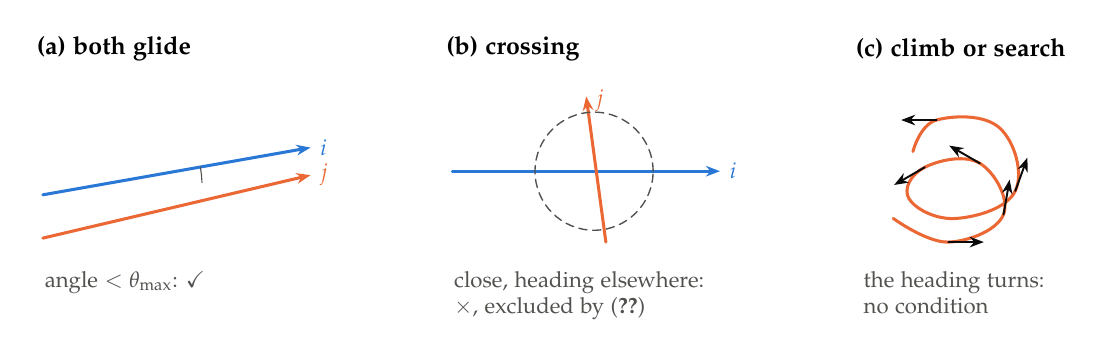
\begin{tikzpicture}[x=1cm,y=1cm]
  \begin{scope}
    \node[panel] at (0,2.75) {(a) both glide};
    \draw[track i, ->] (0.2,0.9) -- (3.6,1.5);
    \draw[track j, ->] (0.2,0.35) -- (3.6,1.15);
    \draw[ink2] (2.2,1.25) arc (10:2:1.4);
    \node[note, align=left, anchor=north west] at (0.1,0.05) {angle $<\theta_{\max}$: \checkmark};
    \node[lbl, blueI, right] at (3.6,1.5) {$i$};
    \node[lbl, orangeJ, right] at (3.6,1.15) {$j$};
  \end{scope}
  \begin{scope}[shift={(5.2,0)}]
    \node[panel] at (0,2.75) {(b) crossing};
    \draw[track i, ->] (0.2,1.2) -- (3.6,1.2);
    \draw[track j, ->] (2.15,0.3) -- (1.9,2.15);
    \draw[tol] (2.0,1.2) circle (0.75);
    \node[note, align=left, anchor=north west] at (0.1,0.05) {close, heading elsewhere:\\$\times$, excluded by~\eqref{eq:heading}};
    \node[lbl, blueI, right] at (3.6,1.2) {$i$};
    \node[lbl, orangeJ, right] at (1.9,2.1) {$j$};
  \end{scope}
  \begin{scope}[shift={(10.4,0)}]
    \node[panel] at (0,2.75) {(c) climb or search};
    \draw[track j] plot[smooth, tension=0.7] coordinates {(0.6,0.6) (1.3,0.3) (2.0,0.65) (1.7,1.3) (1.0,1.25) (0.8,0.85) (1.4,0.6) (2.15,0.95) (1.95,1.75) (1.15,1.85) (0.85,1.45)};
    \foreach \p/\a in {(1.3,0.3)/0, (2.0,0.65)/80, (1.7,1.3)/150, (1.0,1.25)/210, (2.15,0.95)/70, (1.15,1.85)/180}
      \draw[->, ink, line width=0.7pt] \p -- ++(\a:0.45);
    \node[note, align=left, anchor=north west] at (0.1,0.05) {the heading turns:\\no condition};
  \end{scope}
\end{tikzpicture}
\caption{The heading condition~\eqref{eq:heading}. (a) Two gliders on the same route: their
headings differ by less than $\theta_{\max}$. (b) A glider that crosses the area of $i$ heading
elsewhere is close, and the condition excludes it. (c) In a climb or a search the heading turns
continuously and says nothing about the route: the condition is off.}
\label{fig:heading}
\end{figure}

\subsection{The role of each term}\label{sec:roles}

\paragraph{Delay.} With $t'=t$ the condition is simultaneous proximity; with $t'\ne t$ it
recognises similar but shifted tracks, the case of (R2)--(R3). If $t'>t$, $j$ passes where $i$
was, later: $j$ follows $i$. In Figure~\ref{fig:contact} all of $\M_{ij}$ lies above the
diagonal.

\paragraph{Horizontal tolerance.} $\varepsilon_h$ translates the ``nearby places'' of (R3): the
tracks need not pass through the same points.

\paragraph{Vertical tolerance.} In a thermal, $j$ circles over the same spot for minutes, with a
typical spiral radius of 20--26~m~\cite{akos2008}. The horizontal distance
$\|\x_i(t)-\x_j(t+l)\|$ stays far below $\varepsilon_h$ for every delay $l$ of the stay
(Figure~\ref{fig:clock}, top right): without $\varepsilon_z$, any two pilots in the same thermal
would be in contact, whatever their heights. During the climb at rate $w$, pilot $j$ gains $wl$
metres in $l$ seconds:
\begin{equation}\label{eq:climb}
  z_j(t+l)\simeq z_j(t)+w\,l .
\end{equation}
Write $\Delta z = z_i(t)-z_j(t)$ for how far $j$ is below $i$ at time $t$. The vertical condition
then reads
\begin{equation*}
  |z_i(t)-z_j(t+l)|<\varepsilon_z
  \iff |\Delta z - w\,l| < \varepsilon_z
  \iff \Delta z-\varepsilon_z < w\,l < \Delta z+\varepsilon_z ,
\end{equation*}
that is, dividing by $w>0$,
\begin{equation}\label{eq:window}
  l\in\left(\frac{z_i(t)-z_j(t)-\varepsilon_z}{w},\ \frac{z_i(t)-z_j(t)+\varepsilon_z}{w}\right),
\end{equation}
an interval of width $2\varepsilon_z/w$ around $\Delta z/w$, the time $j$ needs to reach the
altitude of $i$. A correspondence exists as long as this interval meets $[-\delta,\delta]$, that
is for $|\Delta z|<\varepsilon_z+w\delta$: at $w=2$~m/s, 900~m of height difference with the
starting $\delta=5$~min and 540~m with the chosen $\delta=2$~min. Two pilots in the same thermal
farther apart in height are not in contact. In a search $w\simeq0$ and the condition reduces to
$|\Delta z|<\varepsilon_z$.

\begin{figure}
\centering
\animated{altitude_clock}
\caption{\animmark The vertical condition in a thermal, for one instant $t$ and every delay $l$;
the animation runs the delay $l$ from $-300$ to $300$~s. Left: $i$ and $j$ in the same thermal,
$j$ lower by $\Delta z=200$~m; the band is $z_i(t)\pm\varepsilon_z$. Top right: the horizontal
distance between $\x_i(t)$ and $\x_j(t+l)$; inside the thermal it never exceeds 50~m, far below
$\varepsilon_h=500$~m, so the horizontal condition alone accepts every delay of the stay; it has
an equal minimum at every turn, so it cannot fix the delay $l^*$ (Section~\ref{sec:phase3}).
Middle right: the altitude of $j$ at $t+l$ crosses the band in a single window. Bottom: the
delays that satisfy each condition and both; both hold for $-50<l<250$~s, the
interval~\eqref{eq:window}, centred on $\Delta z/w=100$~s, and the scan keeps those with
$|l|\le\delta$: $-50<l\le120$~s with $\delta=2$~min.
Before $l=-120$~s, $j$ was gliding towards the thermal: at $l\approx-280$~s it had the right
altitude but was 1.4~km away. Model: $j$ circles with radius 25~m, one turn every 20~s, climbing at
$w=2$~m/s; it arrives at 9~m/s, sinking at 1~m/s; $i$ is on the same circle.}
\label{fig:clock}
\end{figure}

\paragraph{Why not an isotropic 3D distance.} Horizontally a group spreads over scales of a
kilometre, vertically it overlaps within a few hundred metres. A single $\varepsilon$ in
$\|\Delta\x\|_{3D}<\varepsilon$ either makes altitude irrelevant, if it is of the order of a
kilometre, or penalises the normal horizontal spread in glide, if it is of the order of 300~m
(Figure~\ref{fig:isotropic}).

\begin{figure}
\centering
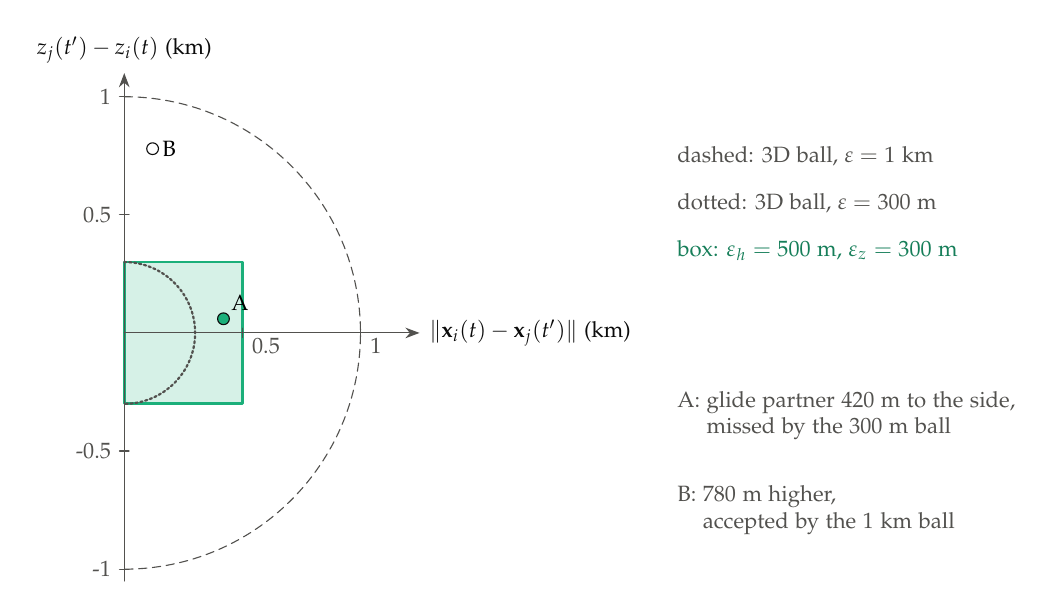
\begin{tikzpicture}[x=3cm,y=3cm]
  \fill[aqua!18] (0,-0.3) rectangle (0.5,0.3);
  \draw[aqua, line width=1pt] (0,-0.3) rectangle (0.5,0.3);
  \draw[ink2, densely dashed] (0,1) arc (90:-90:1);
  \draw[ink2, densely dotted, line width=0.8pt] (0,0.3) arc (90:-90:0.3);
  \draw[->, ink2] (0,0) -- (1.25,0) node[right, lbl, ink] {$\|\x_i(t)-\x_j(t')\|$ (km)};
  \draw[->, ink2] (0,-1.05) -- (0,1.1) node[above, lbl, ink] {$z_j(t')-z_i(t)$ (km)};
  \foreach \v in {0.5,1} \draw[ink2] (\v,-0.02) -- (\v,0.02) node[below right=0pt, lbl] {\v};
  \foreach \v in {-1,-0.5,0.5,1} \draw[ink2] (-0.02,\v) -- (0.02,\v) node[left=3pt, lbl] {\v};
  \node[pt k] (A) at (0.42,0.06) {};
  \node[lbl, above right=-1pt] at (A) {A};
  \node[pt] (B) at (0.12,0.78) {};
  \node[lbl, right] at (B) {B};
  \node[note, align=left, anchor=west] at (2.3,0.75) {dashed: 3D ball, $\varepsilon=1$~km};
  \node[note, align=left, anchor=west] at (2.3,0.55) {dotted: 3D ball, $\varepsilon=300$~m};
  \node[note, align=left, anchor=west, text=aqua!70!ink] at (2.3,0.35) {box: $\varepsilon_h=500$~m, $\varepsilon_z=300$~m};
  \node[note, align=left, anchor=west] at (2.3,-0.35) {A: glide partner 420 m to the side,\\\phantom{A: }missed by the 300 m ball};
  \node[note, align=left, anchor=west] at (2.3,-0.75) {B: 780 m higher,\\\phantom{B: }accepted by the 1 km ball};
\end{tikzpicture}
\caption{Tolerance regions for the separation between $(\x_i(t),z_i(t))$ and $(\x_j(t'),z_j(t'))$.
The box of~\eqref{eq:correspondences} is wide and flat, like a group: it keeps A and rejects B.
A single 3D radius either rejects A or accepts B.}
\label{fig:isotropic}
\end{figure}

\paragraph{Heading only in glide.} In glide the path is nearly straight and $\vh$ is the
direction of the route: condition~\eqref{eq:heading} excludes a pilot who crosses the same area
heading elsewhere (Figure~\ref{fig:heading}). In a climb the heading turns by $2\pi$ in about
twenty seconds and carries no information on the route. In a search the pilot turns often, with
partial circles and changes of heading, and the instantaneous heading says little about the route
too: the condition is off whenever one of the two pilots is not in \st{transition}, unclassified
fixes included. A rejected alternative is the velocity averaged over a window of a few minutes,
with a minimum speed: in a long thermal without wind the mean velocity is nearly zero, and the
threshold would remove the contacts exactly while two pilots share the thermal.

\subsection{Choice of the maximum delay}\label{sec:delta}

If $j$ retraces the track of $i$ with a constant delay $\ell$, $\x_j(t)=\x_i(t-\ell)$, the
distance between the two pilots at the same instant is the distance between two points of the
track of $i$ flown $\ell$ apart,
\[
  \|\x_i(t)-\x_j(t)\| = \|\x_i(t)-\x_i(t-\ell)\| \le v_{\max}\,\ell ,
\]
and $v_\xc\,\ell$ on average once $\ell$ is longer than a climb--glide cycle, $v_\xc$ being the
mean speed of advance. The distance at the same instant grows with the delay. Requiring that two
pilots shifted by any delay up to $\delta$ stay within visual range means
$v_\xc\,\delta\le\varepsilon_\vis$ (Figure~\ref{fig:delta}):
\begin{equation}\label{eq:delta}
  \delta\lesssim\frac{\varepsilon_\vis}{v_\xc},
\end{equation}
so $\delta\approx5$~min for $\varepsilon_\vis\approx1.5$~km and $v_\xc\approx5$~m/s. The speed
$v_\xc$ must be measured on the data, for example as the daily median of the speed of advance
over 30-minute windows. The bound gives the largest admissible delay, not the one at which
following ends; on the data that one was measured directly and is 2~min
(\texttt{method\_assessment.pdf}).

\begin{figure}
\centering
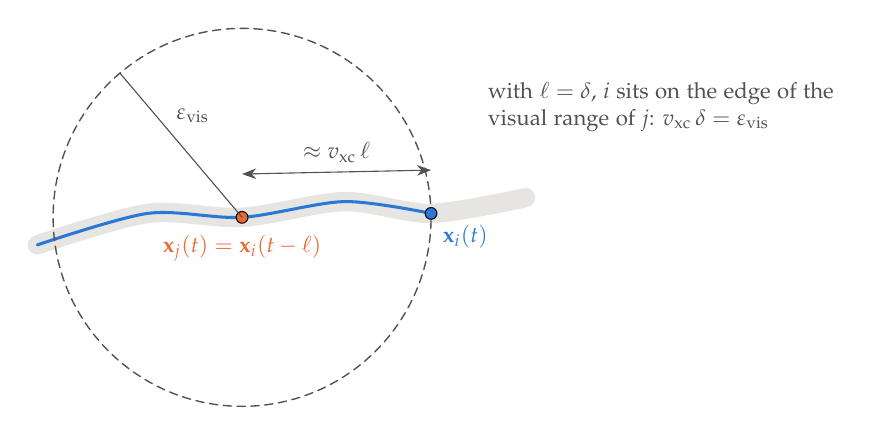
\begin{tikzpicture}[x=1cm,y=1cm]
  \draw[light, line width=7pt] plot[smooth] coordinates {(-2.6,-0.35) (-1.2,0.05) (0,0) (1.3,0.2) (2.4,0.05) (3.6,0.25)};
  \draw[track i] plot[smooth] coordinates {(-2.6,-0.35) (-1.2,0.05) (0,0) (1.3,0.2) (2.4,0.05)};
  \draw[tol] (0,0) circle (2.4);
  \node[pt j] (j) at (0,0) {};
  \node[pt i] (i) at (2.4,0.05) {};
  \node[lbl, orangeJ, below=3pt] at (j) {$\x_j(t)=\x_i(t-\ell)$};
  \node[lbl, blueI, below right=1pt] at (i) {$\x_i(t)$};
  \draw[<->, ink2] (0,0.55) -- node[above, lbl] {$\approx v_\xc\,\ell$} (2.4,0.6);
  \draw[ink2] (0,0) -- (-1.55,1.83) node[pos=0.6, above right=-1pt, lbl] {$\varepsilon_\vis$};
  \node[note, align=left, anchor=west] at (3.0,1.4) {with $\ell=\delta$, $i$ sits on the edge of the\\visual range of $j$: $v_\xc\,\delta=\varepsilon_\vis$};
\end{tikzpicture}
\caption{Choice of the maximum delay. A pilot that retraces the route of $i$ with delay $\ell$ is
about $v_\xc\ell$ behind; the dashed circle is the visual range around $j$. The largest delay that
keeps $i$ in sight is $\delta=\varepsilon_\vis/v_\xc$.}
\label{fig:delta}
\end{figure}

\begin{remark}[two notions of ``together'']\label{rem:notions}
Flying together may mean \emph{seeing each other}, and so being able to use social information,
or \emph{exploiting the same air masses}. The two notions can be written as indicators:
\begin{align*}
  \text{visual co-presence:}\quad & V_{ij}(t) = \ind\Bigl[\bigl\|\bigl(\x_i(t),z_i(t)\bigr)-\bigl(\x_j(t),z_j(t)\bigr)\bigr\|<\varepsilon_\vis\Bigr],\\
  \text{shared air:}\quad & m_{ij}(t) = \ind\bigl[\exists\, |l|\le\delta:\ \|\x_i(t)-\x_j(t+l)\|<\varepsilon_h,\\
  & \hphantom{m_{ij}(t) = \ind\bigl[\exists\, |l|\le\delta:\ }|z_i(t)-z_j(t+l)|<\varepsilon_z,\ D_{ij}(t,t+l)=1\bigr].
\end{align*}
Visual contact depends on the 3D distance and is simultaneous; exploiting the same thermals needs
tight tolerances, vertical ones included, and admits a delay. Definition~\ref{def:contact} with $\varepsilon_z$
of a few hundred metres is the second notion, restricted to the visual range
by~\eqref{eq:delta}. Widening $\varepsilon_z$ brings the criterion closer to visual contact alone.
The value of $\varepsilon_z$ is therefore a choice of definition, to be declared
(Figure~\ref{fig:notions}).
\end{remark}

\begin{figure}
\centering
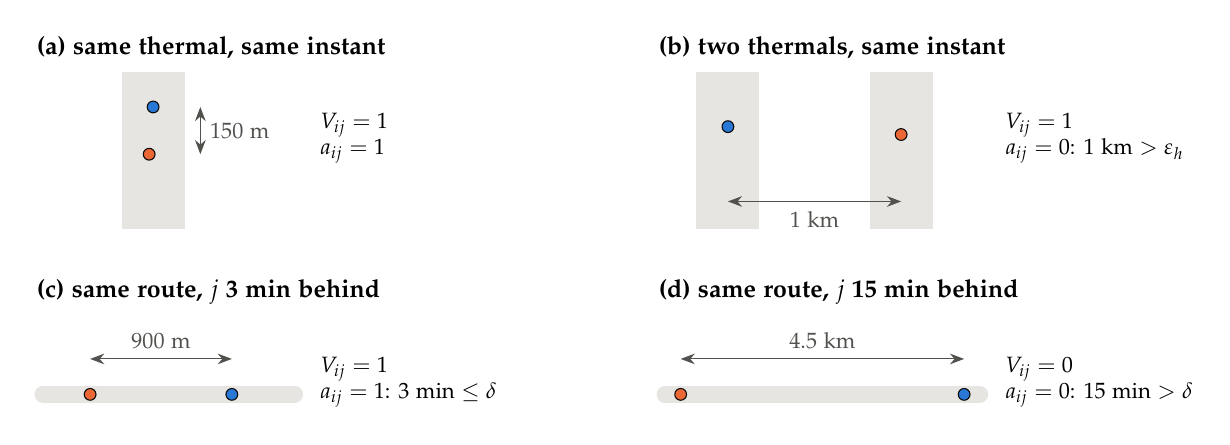
\begin{tikzpicture}[x=1cm,y=1cm,
    verdict/.style={font=\footnotesize, anchor=north west, align=left}]
  \begin{scope}
    \node[panel] at (0,2.3) {(a) same thermal, same instant};
    \fill[light] (1.2,0) rectangle (2.0,2.0);
    \node[pt i] at (1.6,1.55) {}; \node[pt j] at (1.55,0.95) {};
    \draw[<->, ink2] (2.2,0.95) -- node[right, lbl] {150 m} (2.2,1.55);
    \node[verdict] at (3.6,1.6) {$V_{ij}=1$\\$a_{ij}=1$};
  \end{scope}
  \begin{scope}[shift={(7.9,0)}]
    \node[panel] at (0,2.3) {(b) two thermals, same instant};
    \fill[light] (0.6,0) rectangle (1.4,2.0);
    \fill[light] (2.8,0) rectangle (3.6,2.0);
    \node[pt i] at (1.0,1.3) {}; \node[pt j] at (3.2,1.2) {};
    \draw[<->, ink2] (1.0,0.35) -- node[below, lbl] {1 km} (3.2,0.35);
    \node[verdict] at (4.4,1.6) {$V_{ij}=1$\\$a_{ij}=0$: 1 km $>\varepsilon_h$};
  \end{scope}
  \begin{scope}[shift={(0,-3.1)}]
    \node[panel] at (0,2.3) {(c) same route, $j$ 3 min behind};
    \draw[light, line width=6pt] (0.2,1.0) -- (3.4,1.0);
    \node[pt j] at (0.8,1.0) {}; \node[pt i] at (2.6,1.0) {};
    \draw[<->, ink2] (0.8,1.45) -- node[above, lbl] {900 m} (2.6,1.45);
    \node[verdict] at (3.6,1.6) {$V_{ij}=1$\\$a_{ij}=1$: 3 min $\le\delta$};
  \end{scope}
  \begin{scope}[shift={(7.9,-3.1)}]
    \node[panel] at (0,2.3) {(d) same route, $j$ 15 min behind};
    \draw[light, line width=6pt] (0.2,1.0) -- (4.2,1.0);
    \node[pt j] at (0.4,1.0) {}; \node[pt i] at (4.0,1.0) {};
    \draw[<->, ink2] (0.4,1.45) -- node[above, lbl] {4.5 km} (4.0,1.45);
    \node[verdict] at (4.4,1.6) {$V_{ij}=0$\\$a_{ij}=0$: 15 min $>\delta$};
  \end{scope}
\end{tikzpicture}
\caption{Visual co-presence $V_{ij}$ and contact $a_{ij}$ in four situations, with
$\varepsilon_\vis=1.5$~km, $\delta=5$~min and $v_\xc=5$~m/s. In (d), a delay of 15~minutes would
put the two pilots in contact although they cannot see each other: this is what the
bound~\eqref{eq:delta} prevents.}
\label{fig:notions}
\end{figure}

\section{From pairs to groups}\label{sec:groups}

Who flies with whom, as a group? The contact links two pilots at a time: it flickers, it is not
transitive, and it changes during the afternoon. This section turns it into groups in four steps:
pair intervals, groups at each instant (configurations), chains of groups (episodes), and the
flights tied by them (dependency blocks).

\subsection{Pair intervals}\label{sec:pair-intervals}

The instantaneous contact flickers wherever a quantity sits close to its threshold (a distance
near $\varepsilon_h$, a height difference near $\varepsilon_z$, an angle near $\theta_{\max}$), at
the changes of state, where the heading condition switches on and off, and where the phase
labelling is wrong on a few fixes.

\begin{definition}[pair interval]\label{def:pair-interval}
For each pair consider the maximal runs of consecutive grid instants with $a_{ij}=1$. Two runs
separated by a gap shorter than $g$ are joined; the resulting runs shorter than $\tau^*$ are
dropped. Each remaining run is a half-open interval $[t_{\rm on}, t_{\rm off})$, and the set of
the intervals of the day is $\I$.
\end{definition}

Joining the short gaps plays the role of the robustness of Buchin et al.~\cite[§4]{buchin2015},
which ignores interruptions shorter than $\alpha$; the maximal segments of Li et
al.~\cite{li2013,ruzzo1999} are an alternative. The minimum duration $\tau^*$ keeps chance
contacts out, and the null model fixes it (Section~\ref{sec:calibration}).

\begin{figure}
\centering
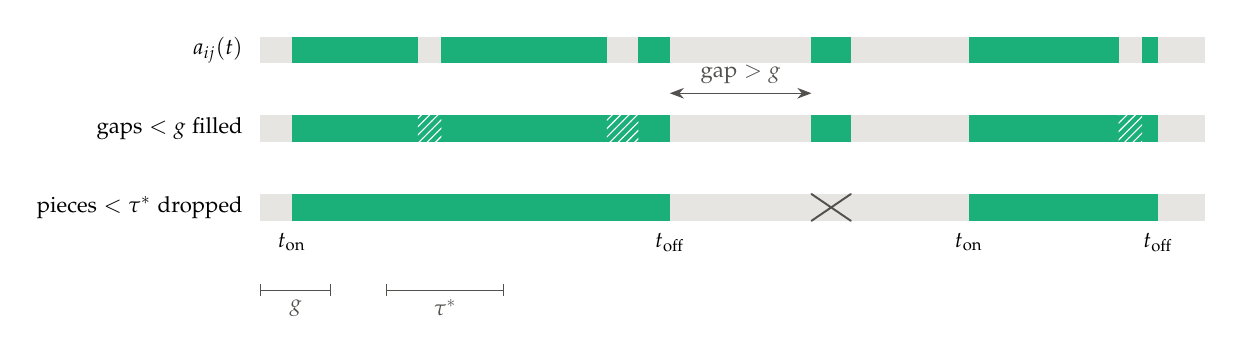
\begin{tikzpicture}[x=1.0cm,y=1cm,
    row/.style={font=\footnotesize, anchor=east}]
  \foreach \y in {2,1,0} \fill[light] (0,\y-0.17) rectangle (12,\y+0.17);
  \node[row] at (-0.1,2) {$a_{ij}(t)$};
  \node[row] at (-0.1,1) {gaps $<g$ filled};
  \node[row] at (-0.1,0) {pieces $<\tau^*$ dropped};
  \foreach \a/\b in {0.4/2.0, 2.3/4.4, 4.8/5.2, 7.0/7.5, 9.0/10.9, 11.2/11.4} \fill[aqua] (\a,1.83) rectangle (\b,2.17);
  \foreach \a/\b in {0.4/5.2, 7.0/7.5, 9.0/11.4} \fill[aqua] (\a,0.83) rectangle (\b,1.17);
  \foreach \a/\b in {2.0/2.3, 4.4/4.8, 10.9/11.2} \fill[pattern=north east lines, pattern color=white] (\a,0.83) rectangle (\b,1.17);
  \foreach \a/\b in {0.4/5.2, 9.0/11.4} \fill[aqua] (\a,-0.17) rectangle (\b,0.17);
  \draw[ink2, line width=0.7pt] (7.0,-0.17) -- (7.5,0.17) (7.0,0.17) -- (7.5,-0.17);
  \foreach \x/\l in {0.4/t_{\rm on}, 5.2/t_{\rm off}, 9.0/t_{\rm on}, 11.4/t_{\rm off}} \node[lbl, below] at (\x,-0.2) {$\l$};
  \draw[<->, ink2] (5.2,1.45) -- node[above, lbl] {gap $>g$} (7.0,1.45);
  \draw[|-|, ink2] (0,-1.05) -- node[below, lbl] {$g$} (0.9,-1.05);
  \draw[|-|, ink2] (1.6,-1.05) -- node[below, lbl] {$\tau^*$} (3.1,-1.05);
\end{tikzpicture}
\caption{From the contact to the pair intervals. Top: the contact of one pair, with the flicker
of the instantaneous condition. Middle: gaps shorter than $g$ are filled (hatched). Bottom: runs
shorter than $\tau^*$ are dropped; two intervals remain.}
\label{fig:pair-intervals}
\end{figure}

\subsection{The problem of non-transitivity}\label{sec:transitivity}

If 1 flies with 8 early in the afternoon and 8 with 14 later, 1 and 14 may never have met: contact
is symmetric but not transitive. A partition into groups needs an \emph{equivalence relation}
$\sim$, reflexive ($i\sim i$), symmetric ($i\sim j\Rightarrow j\sim i$) and transitive ($i\sim j$
and $j\sim k\Rightarrow i\sim k$), so any definition of groups must give up something
(Figure~\ref{fig:transitivity}):
\begin{enumerate}[label=(\alph*)]
  \item direct contact between all members: the transitive closure puts 1 and 14 in one group
        although they never met;
  \item the partition: groups may overlap, here $\{1,8\}$ and $\{8,14\}$, as the maximal groups
        of Buchin et al.~\cite{buchin2015} do;
  \item the static picture: the groups are defined instant by instant.
\end{enumerate}
We take (c): at every instant the groups are the connected components of the graph of active
contacts, as the components of~\cite{buchin2015}, and their evolution is described without
giving a group a lasting identity.

\begin{figure}
\centering
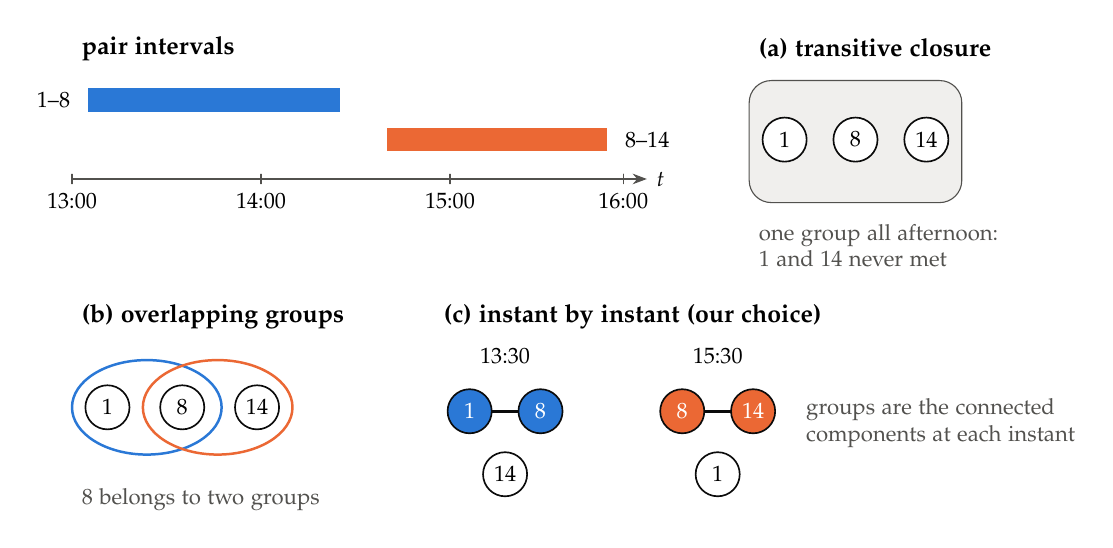
\begin{tikzpicture}[x=1cm,y=1cm]
  \begin{scope}
    \draw[->, ink2] (0,0) -- (7.3,0) node[right, lbl, ink] {$t$};
    \foreach \x/\h in {0/13:00, 2.4/14:00, 4.8/15:00, 7.0/16:00} {
      \draw[ink2] (\x,-0.06) -- (\x,0.06); \node[lbl, below] at (\x,-0.06) {\h};
    }
    \fill[blueI] (0.2,0.85) rectangle (3.4,1.15);
    \node[lbl, anchor=east] at (0.1,1.0) {1--8};
    \fill[orangeJ] (4.0,0.35) rectangle (6.8,0.65);
    \node[lbl, anchor=west] at (6.9,0.5) {8--14};
    \node[panel] at (0,1.65) {pair intervals};
  \end{scope}
  \begin{scope}[shift={(8.6,0)}]
    \node[panel] at (0,1.65) {(a) transitive closure};
    \draw[ink2, rounded corners=8pt, fill=light!60] (0,-0.3) rectangle (2.7,1.25);
    \node[flight] at (0.45,0.5) {1}; \node[flight] at (1.35,0.5) {8}; \node[flight] at (2.25,0.5) {14};
    \node[note, anchor=north west, align=left] at (0,-0.45) {one group all afternoon:\\1 and 14 never met};
  \end{scope}
  \begin{scope}[shift={(0,-3.4)}]
    \node[panel] at (0,1.65) {(b) overlapping groups};
    \draw[blueI, line width=0.9pt] (0.95,0.5) ellipse (0.95 and 0.6);
    \draw[orangeJ, line width=0.9pt] (1.85,0.5) ellipse (0.95 and 0.6);
    \node[flight] at (0.45,0.5) {1}; \node[flight] at (1.4,0.5) {8}; \node[flight] at (2.35,0.5) {14};
    \node[note, anchor=north west, align=left] at (0,-0.4) {8 belongs to two groups};
  \end{scope}
  \begin{scope}[shift={(4.6,-3.4)}]
    \node[panel] at (0,1.65) {(c) instant by instant (our choice)};
    \node[lbl] at (0.9,1.15) {13:30};
    \draw[edge] (0.45,0.45) -- (1.35,0.45);
    \node[inE1] at (0.45,0.45) {1}; \node[inE1] at (1.35,0.45) {8}; \node[flight] at (0.9,-0.35) {14};
    \node[lbl] at (3.6,1.15) {15:30};
    \draw[edge] (3.15,0.45) -- (4.05,0.45);
    \node[flight] at (3.6,-0.35) {1}; \node[inE2] at (3.15,0.45) {8}; \node[inE2] at (4.05,0.45) {14};
    \node[note, anchor=west, align=left] at (4.6,0.3) {groups are the connected\\components at each instant};
  \end{scope}
\end{tikzpicture}
\caption{Non-transitivity: 1--8 early in the afternoon, 8--14 later, and 1 and 14 never meet.
The three ways out: (a) one group of all three, (b) two overlapping groups, (c) the groups of
each instant, our choice.}
\label{fig:transitivity}
\end{figure}

\subsection{Configurations}\label{sec:configurations}

The active graph at instant $t$ is
\begin{equation}\label{eq:graph}
  \begin{gathered}
  G(t)=\bigl(V(t),E(t)\bigr),\qquad V(t)=\{i:\ t\in T^\dep_i\},\\
  E(t)=\bigl\{\{i,j\}:\ \exists\,(i,j,t_{\rm on},t_{\rm off})\in\I,\ t\in[t_{\rm on},t_{\rm off})\bigr\}:
  \end{gathered}
\end{equation}
its nodes are the pilots that at $t$ have departed, have not landed and have a position; its edges
are the pairs whose interval contains $t$. A connected component of $G(t)$ with at least two nodes
is a group at instant $t$: its pilots are joined by chains of contacts (Appendix~\ref{app:graphs}
recalls the terms).

\begin{definition}[configuration]
A configuration $c$ is given by a set of flights $M_c$, its members, with $|M_c|\ge2$, and by an
interval of time $[t^{\rm start}_c, t^{\rm end}_c)$, such that $M_c$ is a connected component of
$G(t)$ at every $t$ of the interval and the interval is maximal. We write
$c=\bigl(M_c,[t^{\rm start}_c,t^{\rm end}_c)\bigr)$.
\end{definition}

The members of a configuration are fixed: a pilot who joins or leaves ends it and starts another.
Only the edges among the members may change: an edge that closes a triangle does not create a new
configuration (Figure~\ref{fig:configurations}). The configurations are the edges of the Reeb
graph of~\cite{buchin2015} with at least two entities (Figure~\ref{fig:reeb}), built on delayed
contacts instead of simultaneous proximity.

\begin{figure}
\centering
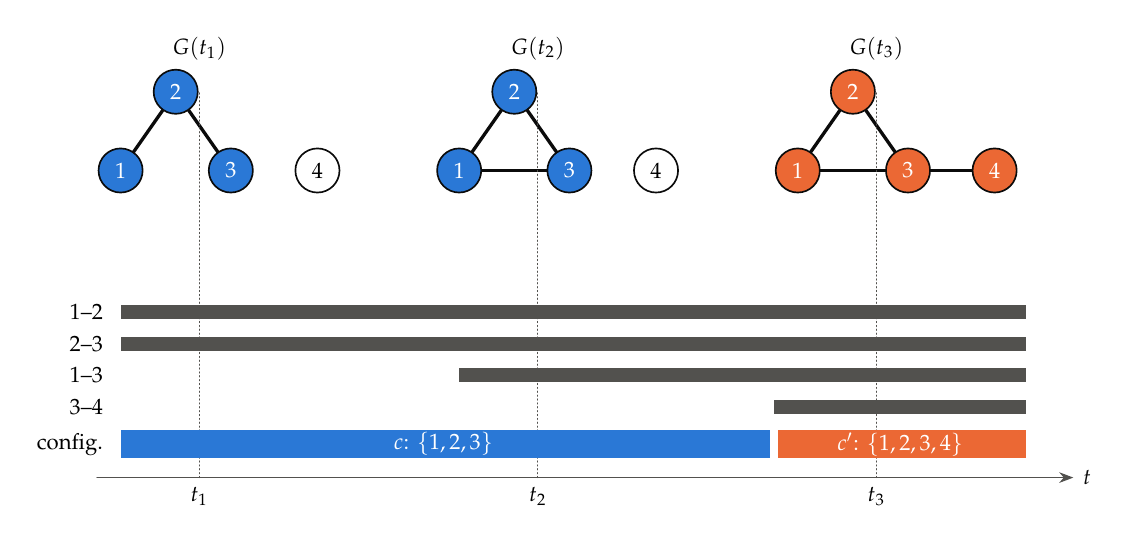
\begin{tikzpicture}[x=1cm,y=1cm]
  \foreach \sx/\t/\tri/\four in {0/t_1/0/0, 4.3/t_2/1/0, 8.6/t_3/1/1} {
    \begin{scope}[shift={(\sx,0)}]
      \node[lbl] at (1.3,2.55) {$G(\t)$};
      \coordinate (a) at (0.3,1.0); \coordinate (b) at (1.0,2.0); \coordinate (c) at (1.7,1.0); \coordinate (d) at (2.8,1.0);
      \draw[edge] (a) -- (b) -- (c);
      \ifnum\tri=1 \draw[edge] (a) -- (c); \fi
      \ifnum\four=1 \draw[edge] (c) -- (d); \fi
      \ifnum\four=1
        \node[inE2] at (a) {1}; \node[inE2] at (b) {2}; \node[inE2] at (c) {3}; \node[inE2] at (d) {4};
      \else
        \node[inE1] at (a) {1}; \node[inE1] at (b) {2}; \node[inE1] at (c) {3}; \node[flight] at (d) {4};
      \fi
    \end{scope}
  }
  \begin{scope}[shift={(0,-2.9)}]
    \draw[->, ink2] (0,0) -- (12.4,0) node[right, lbl, ink] {$t$};
    \foreach \x/\l in {1.3/t_1, 5.6/t_2, 9.9/t_3} {\draw[ink2, densely dotted] (\x,0) -- (\x,4.9); \node[lbl, below] at (\x,0) {$\l$};}
    \foreach \a/\b/\y/\n in {0.3/11.8/2.1/1--2, 0.3/11.8/1.7/2--3, 4.6/11.8/1.3/1--3, 8.6/11.8/0.9/3--4} {
      \fill[ink2] (\a,\y-0.09) rectangle (\b,\y+0.09);
      \node[lbl, anchor=east] at (0.2,\y) {\n};
    }
    \fill[blueI] (0.3,0.25) rectangle (8.55,0.6); \node[font=\footnotesize, text=white] at (4.4,0.425) {$c$: $\{1,2,3\}$};
    \fill[orangeJ] (8.65,0.25) rectangle (11.8,0.6); \node[font=\footnotesize, text=white] at (10.2,0.425) {$c'$: $\{1,2,3,4\}$};
    \node[lbl, anchor=east] at (0.2,0.425) {config.};
  \end{scope}
\end{tikzpicture}
\caption{Configurations. Top: the active graph at three instants. Bottom: the pair intervals of
the four flights and the configurations they produce. At $t_2$ the edge 1--3 closes a triangle:
the component keeps its members and $c$ goes on. When 4 joins, $c$ ends and $c'$ starts.}
\label{fig:configurations}
\end{figure}

\begin{proposition}
At every instant each flight belongs to at most one configuration.
\end{proposition}

\begin{proof}
The connected components of $G(t)$ form a partition of $V(t)$.
\end{proof}

The membership of flight $i$ at instant $t$ is therefore well defined:
\begin{equation}\label{eq:membership}
  \gamma_i(t)=\begin{cases}
    \st{L} & \text{if } k^0_i\le t<k^\dep_i \text{ (local phase), or the flight is local},\\
    c & \text{if } i\in M_c \text{ and } t\in[t^{\rm start}_c,t^{\rm end}_c),\\
    \st{S} & \text{if } t\in T^\dep_i \text{ otherwise (solo flight).}
  \end{cases}
\end{equation}
\fix{In the tables, every instant between the departure and the landing outside a configuration
is labelled \st{S}, the instants in a gap of the track included, where the flight has no position.
The analyses that read the fixes see nothing there; only the time fractions computed from the
membership include them.}

\subsection{Episodes}\label{sec:episodes}

A group that gains or loses a pilot becomes a new configuration, yet its pilots go on flying
together. Episodes keep this continuity.

\begin{definition}[episode]
Two configurations are linked, $c\to c'$, if one starts exactly when the other ends and they have
at least one member in common:
\begin{equation}\label{eq:link}
  c\to c' \iff t^{\rm start}_{c'}=t^{\rm end}_c\ \wedge\ M_c\cap M_{c'}\ne\emptyset .
\end{equation}
An episode is a connected component of the undirected graph associated with $\to$.
\end{definition}

So an episode is a chain of configurations without interruption: each starts when the previous one
ends and keeps at least one of its members, and two configurations of the same episode need not
share anyone. In the language of~\cite{buchin2015}, it is a connected component of the Reeb graph
without the edges of single pilots. Four properties matter (Figure~\ref{fig:episodes}):
\begin{enumerate}[label=(\roman*)]
  \item a split produces two configurations linked to the same previous one, so they stay in the
        same episode; the same holds for a merge;
  \item if the group dissolves completely, the chain breaks and the episode ends; a group that
        forms again later opens a new episode;
  \item no threshold is needed: one member in common is enough;
  \item the same flight can belong to several episodes of the same day, at different times.
\end{enumerate}

\begin{figure}
\centering
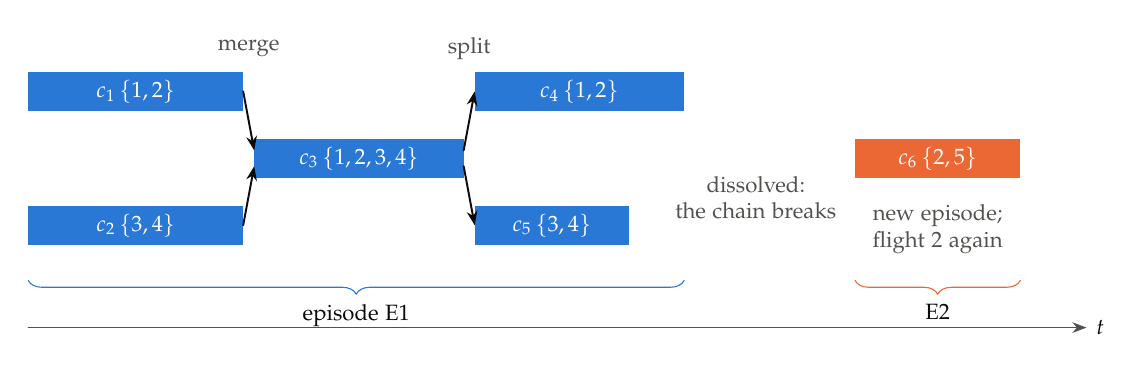
\begin{tikzpicture}[x=1.4cm,y=1cm,
    conf/.style={draw=none, minimum height=5mm, inner sep=0pt, font=\footnotesize, text=white},
    link/.style={->, ink, line width=0.7pt}]
  \draw[->, ink2] (0,-0.4) -- (9.6,-0.4) node[right, lbl, ink] {$t$};
  \def\confbox#1#2#3#4#5{\fill[#5] (#1,#3-0.25) rectangle (#2,#3+0.25); \node[font=\footnotesize, text=white] at ({(#1+#2)/2},#3) {#4};}
  \confbox{0}{1.95}{2.6}{$c_1\,\{1,2\}$}{blueI}
  \confbox{0}{1.95}{0.9}{$c_2\,\{3,4\}$}{blueI}
  \confbox{2.05}{3.95}{1.75}{$c_3\,\{1,2,3,4\}$}{blueI}
  \confbox{4.05}{5.95}{2.6}{$c_4\,\{1,2\}$}{blueI}
  \confbox{4.05}{5.45}{0.9}{$c_5\,\{3,4\}$}{blueI}
  \confbox{7.5}{9.0}{1.75}{$c_6\,\{2,5\}$}{orangeJ}
  \draw[link] (1.95,2.6) -- (2.05,1.85);
  \draw[link] (1.95,0.9) -- (2.05,1.65);
  \draw[link] (3.95,1.85) -- (4.05,2.6);
  \draw[link] (3.95,1.65) -- (4.05,0.9);
  \node[note] at (2.0,3.15) {merge};
  \node[note] at (4.0,3.15) {split};
  \node[note, align=center] at (6.6,1.25) {dissolved:\\the chain breaks};
  \node[note, align=center] at (8.25,0.85) {new episode;\\flight 2 again};
  \draw[decorate, decoration={brace, mirror, amplitude=5pt}, blueI] (0,0.2) -- (5.95,0.2) node[midway, below=5pt, lbl, ink] {episode E1};
  \draw[decorate, decoration={brace, mirror, amplitude=5pt}, orangeJ] (7.5,0.2) -- (9.0,0.2) node[midway, below=5pt, lbl, ink] {E2};
\end{tikzpicture}
\caption{Episodes. Arrows are the links~\eqref{eq:link}. The merge of $c_1$ and $c_2$ into $c_3$
and the split of $c_3$ into $c_4$ and $c_5$ keep all five configurations in episode E1, although
$c_1$ and $c_5$ share no member. After the group dissolves, $c_6$ has no predecessor and opens E2:
flight 2 belongs to both episodes.}
\label{fig:episodes}
\end{figure}

\begin{remark}[why not a persistent group name]
One could keep the same group name while the overlap of the members between two instants exceeds a
threshold, as methods that track communities in evolving networks do with the Jaccard
index~\cite{greene2010}. The choice has three defects: the threshold is arbitrary; a group whose
members are replaced one at a time keeps its name even when none of the first members is left;
in splits and merges no natural criterion says who inherits the name. So we let the episode
record only the continuity, and the configuration the composition.
\end{remark}

\subsection{Dependency blocks}\label{sec:blocks}

Which flights can the statistics treat as independent? Those that never flew in the same episode,
directly or through a chain of episodes.

\begin{definition}[block]
For each day consider the bipartite graph flights--episodes, with an edge between a flight and
every episode it belongs to. Its connected components, restricted to the flights, are the
\emph{dependency blocks}; a flight never in a group is a block on its own.
\end{definition}

\begin{figure}
\centering
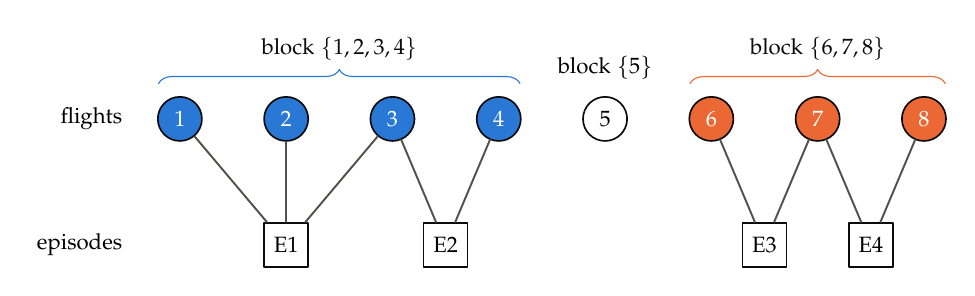
\begin{tikzpicture}[x=1.35cm,y=1cm,
    ep/.style={rectangle, draw=ink, line width=0.6pt, minimum size=5.6mm, inner sep=1pt, font=\footnotesize, fill=white}]
  \foreach \f/\x/\s in {1/0/inE1, 2/1/inE1, 3/2/inE1, 4/3/inE1, 5/4/flight, 6/5/inE2, 7/6/inE2, 8/7/inE2}
    \node[\s] (f\f) at (\x,1.6) {\f};
  \foreach \e/\x in {1/1, 2/2.5, 3/5.5, 4/6.5} \node[ep] (e\e) at (\x,0) {E\e};
  \foreach \e/\f in {1/1, 1/2, 1/3, 2/3, 2/4, 3/6, 3/7, 4/7, 4/8} \draw[ink2, line width=0.7pt] (e\e) -- (f\f);
  \node[lbl, anchor=east] at (-0.45,1.6) {flights};
  \node[lbl, anchor=east] at (-0.45,0) {episodes};
  \draw[decorate, decoration={brace, amplitude=5pt}, blueI] (-0.2,2.05) -- (3.2,2.05) node[midway, above=5pt, lbl, ink] {block $\{1,2,3,4\}$};
  \node[lbl, above=11pt] at (f5) {block $\{5\}$};
  \draw[decorate, decoration={brace, amplitude=5pt}, orangeJ] (4.8,2.05) -- (7.2,2.05) node[midway, above=5pt, lbl, ink] {block $\{6,7,8\}$};
\end{tikzpicture}
\caption{Dependency blocks of a day. Flight 3 is in episodes E1 and E2, so flights 1--4 form one
block although 1 and 4 share no episode; flight 5 never flies in a group.}
\label{fig:blocks}
\end{figure}

\begin{proposition}
The blocks are the finest partition of the flights in which the members of every episode are in
the same block.
\end{proposition}

\begin{proof}
A partition with this property must contain the transitive closure of the relation ``share an
episode'', whose classes are exactly the connected components of the bipartite graph; these, in
turn, satisfy the property.
\end{proof}

The blocks are the units resampled in the bootstrap (Section~\ref{sec:comparison}): flights of
different blocks never shared an episode. Buchin et al.\ already note that a grouping structure
splits the trajectories into independent data sets~\cite[§1]{buchin2015}.

\subsection{An example day}\label{sec:example-day}

Figure~\ref{fig:day} follows a day with five flights. At 11:40 flights 1, 8 and 22 meet (edges
1--8 and 8--22): configuration $c_1=\{1,8,22\}$ starts. At 12:05 the edge 1--22 closes the
triangle: the members do not change and $c_1$ goes on. At 12:55 the interval 1--8 ends as 1
changes route: $c_1$ ends and $c_2=\{8,22\}$ starts; they share 8 and 22, so $c_1\to c_2$. At
13:30 the edge 8--14 opens: $c_3=\{8,14,22\}$, and $c_2\to c_3$. At 14:10 the group dissolves and
episode E1 ends. At 15:00 flights 8 and 22 meet again: $c_4=\{8,22\}$ has no predecessor and
opens episode E2.

So flights 1 and 14 share an episode without ever sharing a configuration; 8 and 22 belong to two
episodes; 1, 8, 14 and 22 form one dependency block, and flight 5, never in a group, a block of
its own.

What we keep from this section: at every instant each flight has one label, \st{L}, \st{S} or its
configuration; configurations chain into episodes, and episodes tie the flights into blocks.
These labels are the output of the method (Appendix~\ref{sec:outputs}). They still depend on
$\tau^*$, which Section~\ref{sec:calibration} fixes.

\begin{figure}
\centering
\animated{example_day}
\caption{\animmark An example day; the animation runs the day from 11:00 to 16:00 and stops at
each event. Top: the active graph $G(t)$ at the five dotted instants; filled nodes are in a
configuration, coloured by episode; dashed nodes are in the local phase, faint ones not in flight. Bottom: the membership $\gamma_i(t)$ of each flight:
hatched is the local phase \st{L}, grey is solo \st{S}, coloured segments are the configurations
$c_1$--$c_4$, and the last row spans the episodes.}
\label{fig:day}
\end{figure}

\section{Algorithm}\label{sec:algorithm}

\algrenewcommand\algorithmicrequire{\textbf{Input:}}
\algrenewcommand\algorithmicensure{\textbf{Output:}}

\begin{figure}
\centering
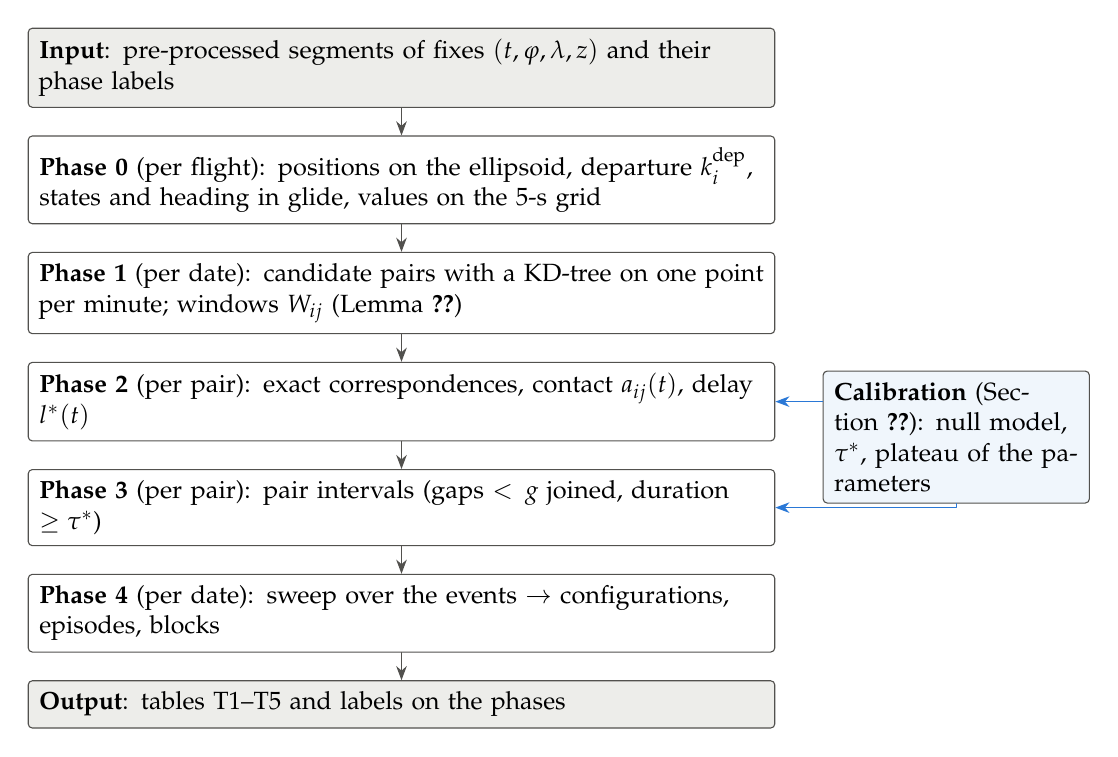
\begin{tikzpicture}[x=1cm,y=1cm,
    stage/.style={draw=ink2, fill=white, rounded corners=1.5pt, text width=9.2cm, align=left, font=\small, inner sep=4pt},
    io/.style={stage, fill=light!70},
    side/.style={draw=ink2, fill=blueI!7, rounded corners=1.5pt, text width=3.1cm, align=left, font=\small, inner sep=4pt}]
  \node[io] (in) at (0,0) {\textbf{Input}: pre-processed segments of fixes $(t,\varphi,\lambda,z)$ and their phase labels};
  \node[stage, below=0.35cm of in] (p0) {\textbf{Phase 0} (per flight): positions on the ellipsoid, departure $k^\dep_i$, states and heading in glide, values on the 5-s grid};
  \node[stage, below=0.35cm of p0] (p1) {\textbf{Phase 1} (per date): candidate pairs with a KD-tree on one point per minute; windows $W_{ij}$ (Lemma~\ref{lem:filter})};
  \node[stage, below=0.35cm of p1] (p2) {\textbf{Phase 2} (per pair): exact correspondences, contact $a_{ij}(t)$, delay $l^*(t)$};
  \node[stage, below=0.35cm of p2] (p3) {\textbf{Phase 3} (per pair): pair intervals (gaps $<g$ joined, duration $\ge\tau^*$)};
  \node[stage, below=0.35cm of p3] (p4) {\textbf{Phase 4} (per date): sweep over the events $\to$ configurations, episodes, blocks};
  \node[io, below=0.35cm of p4] (out) {\textbf{Output}: tables T1--T5 and labels on the phases};
  \foreach \a/\b in {in/p0, p0/p1, p1/p2, p2/p3, p3/p4, p4/out} \draw[->, ink2] (\a) -- (\b);
  \node[side, right=0.6cm of p2.east, anchor=west, yshift=-0.45cm] (cal) {\textbf{Calibration} (Section~\ref{sec:calibration}): null model, $\tau^*$, plateau of the parameters};
  \draw[->, blueI] (cal.west |- p2.east) -- (p2.east);
  \draw[->, blueI] (cal.south) |- (p3.east);
\end{tikzpicture}
\caption{The method as a pipeline. Phases 1--4 work date by date: flights of different days do not
interact, so the computation runs in parallel over the dates and needs the memory of one day.}
\label{fig:pipeline}
\end{figure}

\subsection{Phase 0: preparation per flight}\label{sec:phase0}

\begin{enumerate}[label=(\alph*), leftmargin=2em]
\item \textbf{Positions.} The Earth-centred position of every fix (Section~\ref{sec:data}). One
frame serves all the flights, at any distance and without a map projection, so the coordinates of
two flights compare directly.

\item \textbf{Altitude.} GNSS $z$, unchanged.

\item \textbf{Departure.} $k^\dep_i$ from~\eqref{eq:departure}.

\item \textbf{States and heading.} $s_i(k)$ from the phase labelling. In glide, $\vh_i(k)$ is the
direction of the horizontal velocity, filtered with Savitzky--Golay, in the east and north
directions of the fix itself. Two pilots compared by~\eqref{eq:heading} are less than
$\varepsilon_h$ apart, so their east and north directions differ by less than 0.01\textdegree.

\item \textbf{Grid.} The instants of $\Delta\Z$, with $\Delta=5$~s, the same for all flights. A
grid instant takes the position and the altitude of the fix at that instant or, between two fixes
of the same segment at most $h_{\max}=10$~s apart, the values interpolated linearly between them,
with the state and the heading of the nearer fix; elsewhere the flight has no position. On a
logger that records every second every grid instant is a fix. An interpolated position is at most
$v_{\max}h/2$ from the true one, for two fixes $h$ apart: 69~m at 5~s, 139~m at 10~s.
\end{enumerate}

\begin{doubt}{Is $\Delta=5$~s enough in a thermal?}
Four points per turn do not draw the spiral (Figure~\ref{fig:decimation}), but the contact does
not need its shape. What matters is how far a grid position can be from the track between two
grid instants, compared with the tolerances:
\begin{itemize}[leftmargin=1.2em, itemsep=1pt, topsep=2pt]
  \item horizontally, a pilot is never more than $v_{\max}\Delta/2\approx69$~m from the nearest
        grid point in the worst case, about 20~m while circling at 8~m/s; $\varepsilon_h=500$~m,
        and a whole thermal of radius 25~m fits in a small fraction of it;
  \item vertically, $w\Delta/2=5$~m at 2~m/s and at most 12.5~m at 5~m/s, against
        $\varepsilon_z=300$~m;
  \item on the delay, a grid of 5~s against the $\pm150$~s to which altitude resolves it in a
        thermal (Section~\ref{sec:roles});
  \item on the ends of the intervals, $\pm\Delta$ against $g=120$~s.
\end{itemize}
States and headings are computed on the fixes, before the grid, and lose nothing. The check of
Section~\ref{sec:checks} repeats the computation with $\Delta=1$~s on a subset of 1-Hz pairs.
\end{doubt}

\begin{figure}
\centering
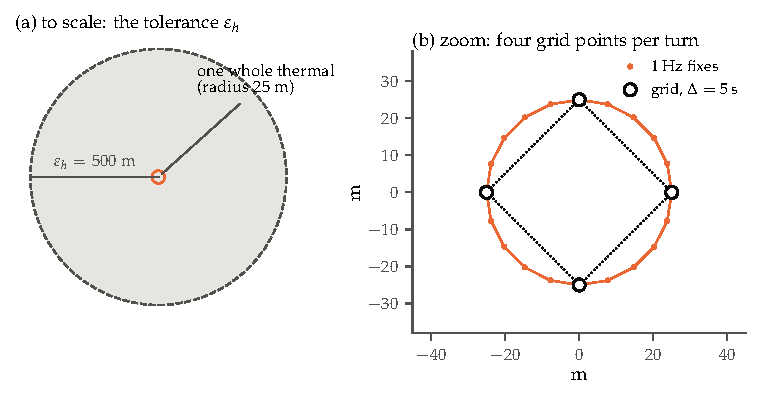
\includegraphics[width=0.92\textwidth]{figures/decimation.pdf}
\caption{The 5-s grid in a thermal, to scale. (a) The horizontal tolerance $\varepsilon_h$ and a whole
thermal of radius 25~m. (b) One turn of 20~s sampled at 1~Hz and on the grid of $\Delta=5$~s:
four grid points per turn, each within 20~m of the 1~Hz fixes around it.}
\label{fig:decimation}
\end{figure}

\begin{table}
\centering
\small
\begin{tabular}{@{}*{7}{l}@{}}
\toprule
\texttt{date} & \texttt{flight} & \texttt{t} & \texttt{X, Y, Z} & \texttt{z} & \texttt{ve, vn} & \texttt{state} \\
\midrule
partition & int32 & int32 (s) & float32 & float32 & float16 & int8 \\
\bottomrule
\end{tabular}
\caption{Table of the grid points, in Parquet partitioned by date: about 30 bytes per row.
\texttt{X, Y, Z} are the Earth-centred position, to 0.5~m in float32; \texttt{ve, vn} the unit
heading in the east and north of the point.}
\label{tab:points}
\end{table}

Under the assumption, to be checked, of $1.86\times10^5$ flights lasting 1.5~h on average, the
table has about $2\times10^8$ rows: 6~GB uncompressed, less in Parquet. It is worth keeping,
because the null model and the calibration read it several times.

\subsection{Phase 1: candidate pairs}\label{sec:phase1}

The exact computation over all pairs of simultaneous flights is wasted effort: almost all of them
never come close. A coarse filter reduces the pairs, with the guarantee of losing none.

The filter works on segments. Let $\tilde\x_i(s)$ be a segment of flight $i$ extended by holding
its first position before it and its last position after it, and let $v_{\max}$ be the top speed
of the pre-processing: within a segment no step between two fixes is faster, because the
excursion rule (step~6) deletes or splits at any faster step, and the interpolation onto the grid
keeps the bound. The filter compares positions at whole minutes, and a minute may fall just before
or just after a segment: the extension gives the track a position there.

\begin{lemma}[no false negative]\label{lem:filter}
If $(t,t')\in\M_{ij}$, $\tilde\x_i$ and $\tilde\x_j$ are the extended segments that contain $t$
and $t'$, and $t_c=60\cdot\mathrm{round}(t/60)$, then
\begin{equation}\label{eq:filter}
  \|\tilde\x_i(t_c)-\tilde\x_j(t_c)\| \le D_c := \varepsilon_h+v_{\max}\,(\delta+60~\mathrm{s}).
\end{equation}
\end{lemma}

\begin{inwords}
$t_c$ is the whole minute nearest to $t$ (Figure~\ref{fig:lemma}a), and both positions
in~\eqref{eq:filter} are read at that \emph{same} instant. If two pilots have a correspondence at
all, then at the nearest whole minute they are less than $D_c$ apart; a pair farther than $D_c$ at
every minute has no correspondence and can be discarded.
\end{inwords}

\begin{proof}
The extension with a fixed position keeps the Lipschitz property
$\|\tilde\x(s)-\tilde\x(s')\|\le v_{\max}|s-s'|$ for all $s,s'$. By construction of $t_c$,
$|t-t_c|\le30$~s, and $|t'-t_c|\le|t'-t|+|t-t_c|\le\delta+30$~s. The triangle inequality along
the path $\tilde\x_i(t_c)\to\x_i(t)\to\x_j(t')\to\tilde\x_j(t_c)$ (Figure~\ref{fig:lemma}) gives
\begin{align*}
  \|\tilde\x_i(t_c)-\tilde\x_j(t_c)\|
  &\le \|\tilde\x_i(t_c)-\x_i(t)\| + \|\x_i(t)-\x_j(t')\| + \|\x_j(t')-\tilde\x_j(t_c)\|\\
  &\le 30\,v_{\max} + \varepsilon_h + v_{\max}(\delta+30),
\end{align*}
where the middle term is below $\varepsilon_h$ because $(t,t')$ is a correspondence
(Definition~\ref{def:correspondence}).
\end{proof}

\begin{figure}
\centering
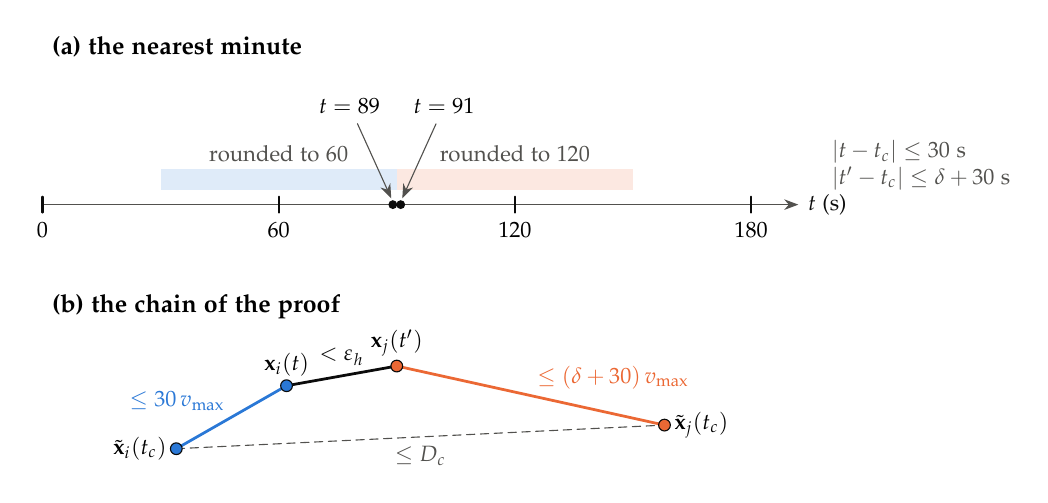
\begin{tikzpicture}[x=1cm,y=1cm]
  \begin{scope}
    \node[panel] at (0,2.0) {(a) the nearest minute};
    \draw[->, ink2] (0,0) -- (9.6,0) node[right, lbl, ink] {$t$ (s)};
    \foreach \x/\l in {0/0, 3/60, 6/120, 9/180} {\draw[ink, line width=0.8pt] (\x,-0.1) -- (\x,0.1); \node[lbl, below] at (\x,-0.1) {\l};}
    \fill[blueI!15] (1.5,0.18) rectangle (4.5,0.45);
    \node[note] at (3.0,0.65) {rounded to 60};
    \fill[orangeJ!15] (4.5,0.18) rectangle (7.5,0.45);
    \node[note] at (6.0,0.65) {rounded to 120};
    \fill[ink] (4.45,0) circle (1.6pt); \node[lbl] (n89) at (3.9,1.25) {$t=89$};
    \draw[->, ink2] (n89) -- (4.43,0.08);
    \fill[ink] (4.55,0) circle (1.6pt); \node[lbl] (n91) at (5.1,1.25) {$t=91$};
    \draw[->, ink2] (n91) -- (4.57,0.08);
    \node[note, anchor=west, align=left] at (9.9,0.5) {$|t-t_c|\le30$~s\\$|t'-t_c|\le\delta+30$~s};
  \end{scope}
  \begin{scope}[shift={(1.5,-3.3)}]
    \node[panel] at (-1.5,2.0) {(b) the chain of the proof};
    \coordinate (a) at (0.2,0.2); \coordinate (b) at (1.6,1.0); \coordinate (c) at (3.0,1.25); \coordinate (d) at (6.4,0.5);
    \draw[blueI, line width=1pt] (a) -- node[above left=-2pt, lbl] {$\le30\,v_{\max}$} (b);
    \draw[ink, line width=1pt] (b) -- node[above, lbl] {$<\varepsilon_h$} (c);
    \draw[orangeJ, line width=1pt] (c) -- node[above right=-2pt, lbl] {$\le(\delta+30)\,v_{\max}$} (d);
    \draw[ink2, densely dashed] (a) -- node[below, lbl] {$\le D_c$} (d);
    \node[pt i] at (a) {}; \node[pt i] at (b) {}; \node[pt j] at (c) {}; \node[pt j] at (d) {};
    \node[lbl, left] at (a) {$\tilde\x_i(t_c)$};
    \node[lbl, above] at (b) {$\x_i(t)$};
    \node[lbl, above] at (c) {$\x_j(t')$};
    \node[lbl, right] at (d) {$\tilde\x_j(t_c)$};
  \end{scope}
\end{tikzpicture}
\caption{Lemma~\ref{lem:filter}. (a) Every instant is at most 30~s from its nearest whole minute.
(b) From $i$ at the minute to $j$ at the same minute through the correspondence $(t,t')$: each step
is bounded by the time it takes at most $v_{\max}$, or by $\varepsilon_h$.}
\label{fig:lemma}
\end{figure}

With $v_{\max}=100$~km/h, $\delta=300$~s and $\varepsilon_h=500$~m, $D_c\approx10.5$~km. The
filter runs as follows, for each date.
\begin{enumerate}
  \item For each segment keep one point per minute of its extended track, for $t_c$ from
        $\delta+60$~s before its first instant after the departure to $\delta+60$~s after its
        last instant. This is the interval in which the lemma may ask for the position, whichever
        of the two roles the flight has.
  \item Build a single KD-tree~\cite{virtanen2020} on the coordinates $(X, Y, Z, K t_c/60)$ with
        $K\gg D_c$, for example $K=10^8$~m: points of different minutes are more than $D_c$ apart
        and are never paired (Figure~\ref{fig:kdtree}).
  \item The search of all pairs within $D_c$ (\texttt{query\_pairs}) returns pairs of points of
        the same minute, hence triples $(i,j,t_c)$; the pairs of two segments of the same flight
        are dropped.
  \item For each candidate pair, with $i<j$, the window is
        $W_{ij}=\bigcup_{t_c}[t_c-30,t_c+30]\cap T^\dep_i$, the union over the minutes $t_c$ at which
        the pair passed the filter: a set of instants of the flight of $i$.
\end{enumerate}
By the lemma, every correspondence $(t,t')\in\M_{ij}$ has $t\in W_{ij}$. The cost is
$O(n_d\log n_d)$ per date, with $n_d$ the number of points per minute of the day. Phase~1 is worth
running on the whole dataset before Phase~2: the number of pairs and the total duration of the
windows give a precise estimate of the cost that follows.

\begin{figure}
\centering
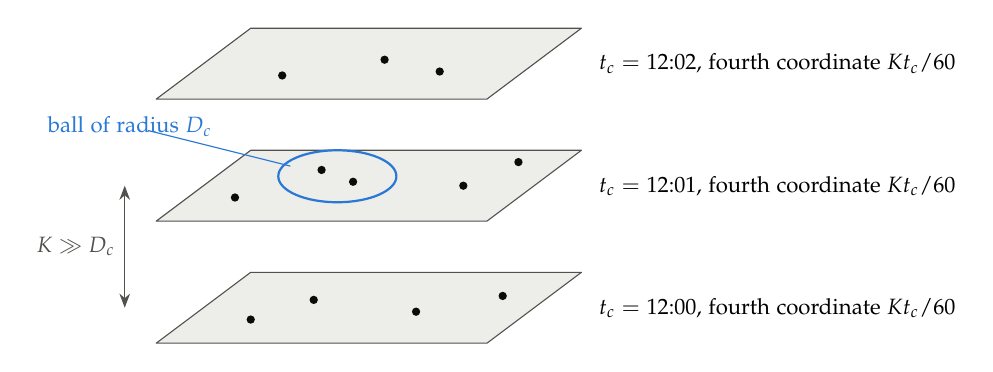
\begin{tikzpicture}[x=1cm,y=1cm]
  \foreach \k/\h in {0/12{:}00, 1/12{:}01, 2/12{:}02} {
    \begin{scope}[shift={(0,1.55*\k)}]
      \fill[light!70] (0,0) -- (4.2,0) -- (5.4,0.9) -- (1.2,0.9) -- cycle;
      \draw[ink2, line width=0.4pt] (0,0) -- (4.2,0) -- (5.4,0.9) -- (1.2,0.9) -- cycle;
      \node[lbl, anchor=west] at (5.5,0.45) {$t_c=$ \h, fourth coordinate $K t_c/60$};
    \end{scope}
  }
  \foreach \p in {(1.2,0.3),(2.0,0.55),(3.3,0.4),(4.4,0.6)} \fill[ink] \p circle (1.5pt);
  \foreach \p in {(1.0,1.85),(2.1,2.2),(2.5,2.05),(3.9,2.0),(4.6,2.3)} \fill[ink] \p circle (1.5pt);
  \foreach \p in {(1.6,3.4),(2.9,3.6),(3.6,3.45)} \fill[ink] \p circle (1.5pt);
  \draw[blueI, line width=0.8pt] (2.3,2.12) ellipse (0.75 and 0.33);
  \node[lbl, blueI, anchor=west] at (-1.5,2.75) {ball of radius $D_c$};
  \draw[blueI] (-0.1,2.7) -- (1.7,2.25);
  \draw[<->, ink2] (-0.4,0.45) -- node[left, lbl] {$K\gg D_c$} (-0.4,2.0);
\end{tikzpicture}
\caption{The KD-tree of Phase~1. Each minute is a layer of the space $(X,Y,Z,Kt_c/60)$, drawn
here as a plane, and the layers are $K\gg D_c$ apart: a search of radius $D_c$ only finds points of the same minute, so one
tree does the work of one search per minute.}
\label{fig:kdtree}
\end{figure}

\subsection{Phase 2: exact correspondences}\label{sec:phase2}

\begin{lemma}\label{lem:scan}
Scanning the instants $t\in W_{ij}$ and the delays $l\in\Lambda=\{-L\Delta,\dots,L\Delta\}$, with
$L=\lfloor\delta/\Delta\rfloor$, enumerates all pairs of $\M_{ij}$; hence $m_{ij}$ and $m_{ji}$ are
obtained exactly.
\end{lemma}

\begin{proof}
Every $(t,t')\in\M_{ij}$ has $t\in W_{ij}$ (Lemma~\ref{lem:filter}) and $t'-t\in\Lambda$. Moreover
$m_{ji}(t')=1$ if and only if there is a $t$ with $(t,t')\in\M_{ij}$, and every such $t$ lies in
$W_{ij}$.
\end{proof}

\begin{algorithm}[htbp]
\caption{Phase 2: scan of one candidate pair}\label{alg:scan}
\begin{algorithmic}[1]
\Require flights $i<j$, on the grid; window $W\subseteq T^\dep_i$; delays $\Lambda$
\Ensure contact $a$ on the support $W\cup(W+\Lambda)$; delay $l^*$ on $W$
\State $m_{ij}\gets0$;\ $m_{ji}\gets0$;\ $d^{\min}\gets+\infty$;\ $l^*\gets$ undefined
\For{$l\in\Lambda$}
  \State $\tau\gets\{t\in W:\ t+l\in T^\dep_j\}$ \Comment{array of instants}
  \State $d\gets\|\x_i(\tau)-\x_j(\tau+l)\|$;\ $h\gets|z_i(\tau)-z_j(\tau+l)|$
  \State $c\gets(d<\varepsilon_h)\wedge(h<\varepsilon_z)\wedge D_{ij}(\tau,\tau+l)$
  \State $m_{ij}[\tau]\gets m_{ij}[\tau]\vee c$;\ $m_{ji}[\tau+l]\gets m_{ji}[\tau+l]\vee c$
  \State $u\gets c\wedge(d<d^{\min}[\tau])$;\ $d^{\min}[\tau]\gets d$ and $l^*[\tau]\gets l$ where $u$
\EndFor
\State $a(t)\gets m_{ij}(t)\vee m_{ji}(t)$
\State \Return $a$, $l^*$
\end{algorithmic}
\end{algorithm}

Each pass of the loop takes one delay $l$: in the $(t,t')$ plane it is the diagonal $t'=t+l$,
evaluated over the whole window at once (Figure~\ref{fig:scan}). The cost is
$\sum_{\rm pairs}|W_{ij}|\,(2L+1)$ distance evaluations, with $2L+1=121$ for $\delta=5$~min and
$\Delta=5$~s. The memory is $O(|W_{ij}|)$ per pair: boolean arrays are accumulated, without
generating the list of pairs of points. Each step of the loop is a vector operation on arrays.

\begin{figure}
\centering
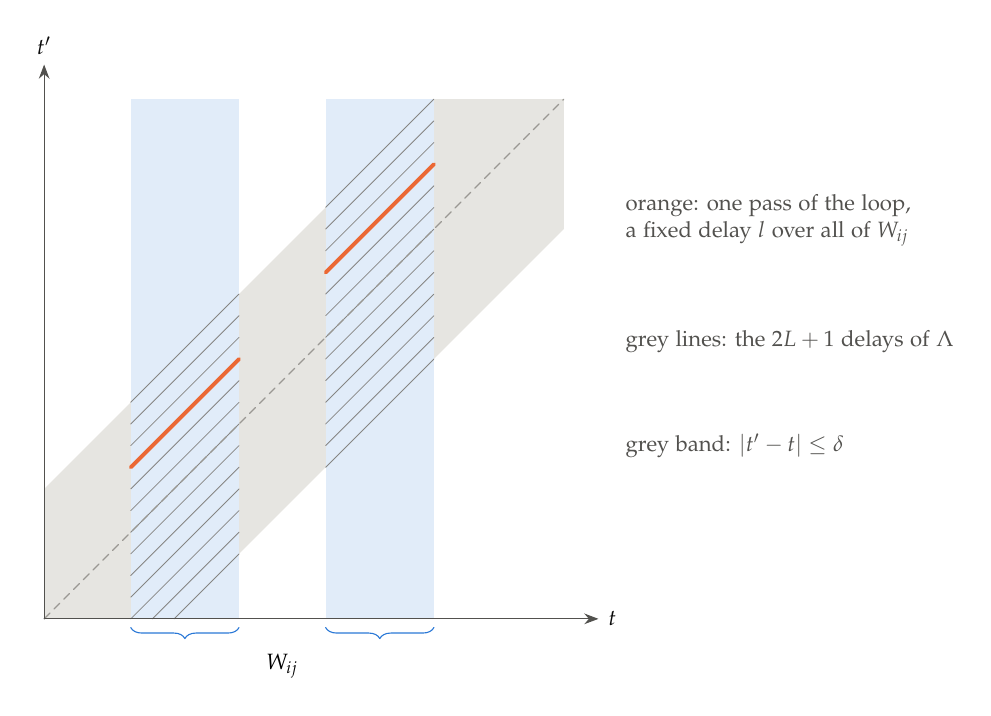
\begin{tikzpicture}[x=0.55cm,y=0.55cm]
  \fill[light] (0,0) -- (3,0) -- (12,9) -- (12,12) -- (9,12) -- (0,3) -- cycle;
  \fill[blueI!14] (2,0) rectangle (4.5,12);
  \fill[blueI!14] (6.5,0) rectangle (9,12);
  \foreach \l in {-3,-2.5,...,3} {
    \draw[ink2!70, line width=0.3pt] ({max(2,-1*\l)},{max(2,-1*\l)+\l}) -- ({min(4.5,12-\l)},{min(4.5,12-\l)+\l});
    \draw[ink2!70, line width=0.3pt] ({max(6.5,-1*\l)},{max(6.5,-1*\l)+\l}) -- ({min(9,12-\l)},{min(9,12-\l)+\l});
  }
  \draw[orangeJ, line width=1.4pt] (2,3.5) -- (4.5,6.0);
  \draw[orangeJ, line width=1.4pt] (6.5,8.0) -- (9,10.5);
  \draw[muted, densely dashed] (0,0) -- (12,12);
  \draw[->, ink2] (0,0) -- (12.8,0) node[right, lbl, ink] {$t$};
  \draw[->, ink2] (0,0) -- (0,12.8) node[above, lbl, ink] {$t'$};
  \draw[decorate, decoration={brace, mirror, amplitude=4pt}, blueI] (2,-0.2) -- (4.5,-0.2);
  \draw[decorate, decoration={brace, mirror, amplitude=4pt}, blueI] (6.5,-0.2) -- (9,-0.2);
  \node[lbl, below=6pt] at (5.5,-0.2) {$W_{ij}$};
  \node[note, anchor=west, align=left] at (13.2,9.2) {orange: one pass of the loop,\\a fixed delay $l$ over all of $W_{ij}$};
  \node[note, anchor=west, align=left] at (13.2,6.4) {grey lines: the $2L+1$ delays of $\Lambda$};
  \node[note, anchor=west, align=left] at (13.2,4.0) {grey band: $|t'-t|\le\delta$};
\end{tikzpicture}
\caption{Phase 2 in the $(t,t')$ plane. Only the columns of the window $W_{ij}$ are scanned, one
diagonal $t'=t+l$ at a time; by Lemma~\ref{lem:scan} this covers all of $\M_{ij}$.}
\label{fig:scan}
\end{figure}

\subsection{Phase 3: pair intervals}\label{sec:phase3}

From the contact $a$ one extracts the runs of 1, joins those separated by gaps shorter than $g$
and keeps those lasting at least $\tau^*$ (Definition~\ref{def:pair-interval}). For each interval one also records:
\begin{itemize}
  \item the signed median delay $\ell_{\rm med}=\mathrm{median}\{l^*(t):\ t\in[t_{\rm on},t_{\rm
        off}),\ m_{ij}(t)=1\}$: if $\ell_{\rm med}>0$, $j$ follows $i$, as in~\cite{li2013}. In a
        search the delay is poorly determined (Section~\ref{sec:roles}), so the instants at which
        either pilot is in \st{search} are better left out of the median;
  \item the distance between the takeoffs $d_{\rm dec}=\|\x_i(k^0_i)-\x_j(k^0_j)\|$, which allows
        requirement (R1) to be imposed afterwards, if wanted.
\end{itemize}

\subsection{Phase 4: configurations and episodes}\label{sec:phase4}

Between one event and the next the set of active edges does not change, so it is enough to update
the components at the instants at which an interval starts or ends, and only around the nodes
involved (Figure~\ref{fig:sweep}).

\begin{algorithm}[htbp]
\caption{Phase 4: sweep over the events of one day}\label{alg:sweep}
\begin{algorithmic}[1]
\Require pair intervals $\I$ of the day
\Ensure configurations; episodes (classes of a union--find)
\State events $\gets\{(t_{\rm on},+,\{a,b\}),\ (t_{\rm off},-,\{a,b\})\}$ sorted in time
\State $A\gets\emptyset$ (active edges);\ $\mathcal{O}\gets\emptyset$ (open configurations)
\For{each instant $t_e$, with its batch of events $B$}
  \State $U\gets$ endpoints of the edges in $B$ \Comment{nodes involved}
  \State $R\gets U\cup\bigcup\{M_c:\ c\in\mathcal{O},\ M_c\cap U\ne\emptyset\}$
  \State update $A$ with the events of $B$
  \State $\mathcal{K}\gets$ connected components of $(R, A|_R)$ with at least two nodes \Comment{local visit}
  \State $X\gets\{c\in\mathcal{O}:\ M_c\subseteq R,\ M_c\notin\mathcal{K}\}$; close every $c\in X$ with $t^{\rm end}_c\gets t_e$
  \For{$K\in\mathcal{K}$ that is not already an open configuration}
    \State open $c'$ with $M_{c'}=K$ and $t^{\rm start}_{c'}=t_e$
    \For{$c\in X$ with $M_c\cap K\ne\emptyset$}
      \State \Call{Union}{$c, c'$}
    \EndFor
  \EndFor
\EndFor
\end{algorithmic}
\end{algorithm}

\begin{lemma}\label{lem:local}
After the update, the connected component of every node of $R$ is contained in $R$; hence the
local recomputation of Algorithm~\ref{alg:sweep} gives the same components as a global one.
\end{lemma}

\begin{proof}
Before the update the open configurations are disjoint, and those that touch $U$ lie entirely in
$R$. A path that starts in $R$ uses old edges, which stay inside the old component, or new edges,
whose endpoints lie in $U\subseteq R$. By induction on the length of the path, every node it
reaches is in $R$.
\end{proof}

\begin{figure}
\centering
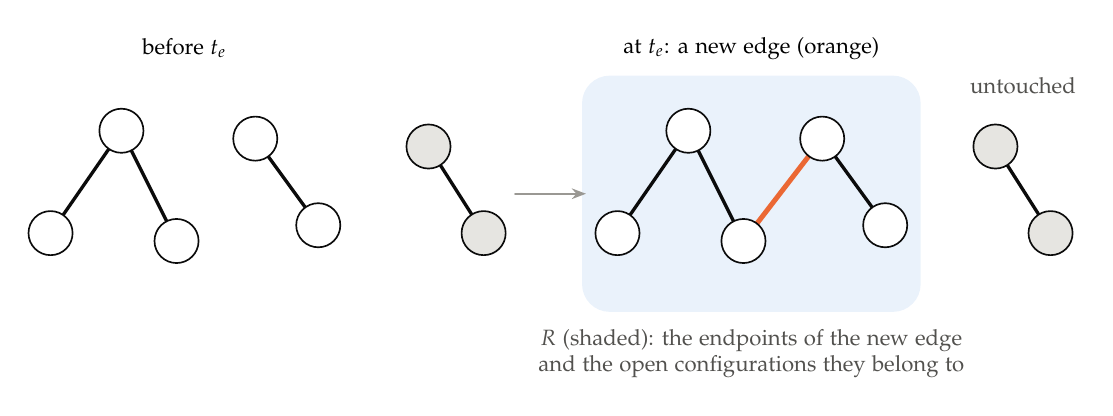
\begin{tikzpicture}[x=1cm,y=1cm]
  \foreach \sx/\new in {0/0, 7.2/1} {
    \begin{scope}[shift={(\sx,0)}]
      \ifnum\new=1 \fill[blueI!10, rounded corners=10pt] (-0.45,-0.5) rectangle (3.85,2.5); \fi
      \coordinate (a) at (0,0.5); \coordinate (b) at (0.9,1.8); \coordinate (c) at (1.6,0.4);
      \coordinate (d) at (2.6,1.7); \coordinate (e) at (3.4,0.6);
      \coordinate (f) at (4.8,1.6); \coordinate (g) at (5.5,0.5);
      \draw[edge] (a) -- (b) -- (c);
      \draw[edge] (d) -- (e);
      \draw[edge] (f) -- (g);
      \ifnum\new=1 \draw[edge, orangeJ, line width=1.8pt] (c) -- (d); \fi
      \foreach \n in {a,b,c,d,e} \node[flight] at (\n) {};
      \node[flight, fill=light] at (f) {}; \node[flight, fill=light] at (g) {};
    \end{scope}
  }
  \node[lbl] at (1.7,2.85) {before $t_e$};
  \node[lbl] at (8.9,2.85) {at $t_e$: a new edge (orange)};
  \node[note, anchor=north, align=center] at (8.9,-0.6) {$R$ (shaded): the endpoints of the new edge\\and the open configurations they belong to};
  \node[note, anchor=south, align=center] at (12.35,2.15) {untouched};
  \draw[->, muted, line width=0.8pt] (5.9,1.0) -- (6.8,1.0);
\end{tikzpicture}
\caption{One step of the sweep. Only the nodes of $R$ are visited again; the grey component far
away keeps its configuration. The animation of Figure~\ref{fig:day} runs the sweep over a whole
day.}
\label{fig:sweep}
\end{figure}

The cost per day is $O(|\I|\log|\I|)$ for the sorting, plus the sum of the sizes of the
components involved at each event, at most a few hundred nodes. The classes of the
union--find~\cite{tarjan1975} are the episodes. From the list of the configurations one obtains
$\gamma_i(t)$ as in~\eqref{eq:membership}, filling with \st{S} the stretches after the departure
not covered by a configuration and with \st{L} the local phase.

\subsection{Costs and space}\label{sec:costs}

\begin{table}
\centering
\small
\begin{tabular}{@{}l l l@{}}
\toprule
Phase & Cost & Data produced \\
\midrule
0 & linear in the number of fixes ($\sim10^9$) & grid points, $\sim2\times10^8$ rows \\
1 & $O(n_d\log n_d)$ per date, $\sum_d n_d\sim1.7\times10^7$ & candidate pairs and windows \\
2 & $\sum|W_{ij}|(2L+1)$; measured after Phase~1 & temporary arrays per pair \\
3 & linear in the duration of the windows & T1, pair intervals \\
4 & $O(|\I|\log|\I|)$ per date & T2--T5 \\
\bottomrule
\end{tabular}
\caption{Costs and space. The numbers assume $1.86\times10^5$ flights of 1.5~h on average and are
to be checked on the data.}
\label{tab:costs}
\end{table}

Phases 1--4 are independent across dates and run in parallel without coordination. Phase~2
dominates the cost; Phase~1 allows it to be estimated before running it.

\section{Calibration: what chance means}\label{sec:calibration}

How many contacts would chance alone give? Pilots who never interact still meet: they take off
from the same site, follow the same ridges and climb in the same house thermals. A contact says
little by itself; what counts is how many contacts of a given duration occur beyond chance.
Interaction indices based on standard tests overestimate the interactions with finely
sampled telemetry~\cite{long2014}, so we build chance from the data, with copies of the flights shifted in
time, and derive from it the shortest duration $\tau^*$ of a contact. The run reported from here
on covers the 162\,485 cleaned flights of 6\,209 dates of the FFVL archive
(Section~\ref{sec:data}).

\subsection{The null model}\label{sec:null}

On each date we draw up to 200 pairs $(i,j)$ of flights whose takeoffs are less than $R_s=10$~km
apart, and replace flight $j$ by its copy shifted in time:
\begin{equation}\label{eq:shift}
  \x^s_j(t)=\x_j(t+r_{ij}),\quad z^s_j(t)=z_j(t+r_{ij}),\qquad
  r_{ij}=(k^0_j-k^0_i)-\vartheta,\quad \vartheta\sim\hat P\bigl(k^0_j-k^0_i\bigr).
\end{equation}
The delay $\vartheta$ is drawn from the delays between the takeoffs of the pairs of that date with
takeoffs within $R_s$: the copy of $j$ takes off $\vartheta$ after $i$, as a real pilot of the
day could. We accept only shifts with $|r_{ij}|\ge r_{\min}=2\delta+\Delta=245$~s, rounded to the
grid step, and a pair enters once, with the roles of $i$ and $j$ drawn at random. The idea of
shifting tracks in time, which keeps the spatial constraints and destroys the synchronisation,
comes from Spiegel et al.~\cite{spiegel2016}, who shuffle whole days of each individual; here a
flight is shifted within its day, against one other flight.

No real correspondence survives the shift (Figure~\ref{fig:null}). If $(t,t')$ was a real
correspondence, in the surrogate pair the position of $j$ at $t'$ comes at $t'-r_{ij}$, at least
$|r_{ij}|-\delta>\delta$ away from $t$. The correspondences that remain are encounters on the same
route without synchrony.

\begin{figure}
\centering
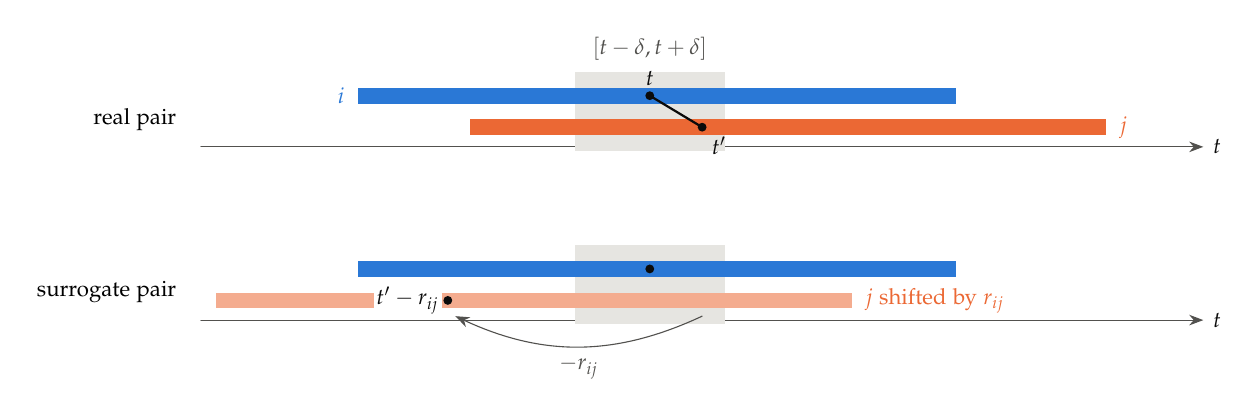
\begin{tikzpicture}[x=0.95cm,y=1cm]
  \foreach \y/\name in {2.2/real pair, 0.0/surrogate pair} \node[lbl, anchor=east] at (-0.2,\y+0.35) {\name};
  \begin{scope}[shift={(0,2.2)}]
    \draw[->, ink2] (0,0) -- (13.4,0) node[right, lbl, ink] {$t$};
    \fill[light] (5.0,-0.05) rectangle (7.0,0.95);
    \fill[blueI] (2.1,0.55) rectangle (10.1,0.75); \node[lbl, blueI, anchor=east] at (2.05,0.65) {$i$};
    \fill[orangeJ] (3.6,0.15) rectangle (12.1,0.35); \node[lbl, orangeJ, anchor=west] at (12.15,0.25) {$j$};
    \draw[ink, line width=0.8pt] (6.0,0.65) -- (6.7,0.25);
    \fill[ink] (6.0,0.65) circle (1.6pt) node[above, lbl] {$t$};
    \fill[ink] (6.7,0.25) circle (1.6pt) node[below right, lbl] {$t'$};
    \node[note] at (6.0,1.25) {$[t-\delta,t+\delta]$};
  \end{scope}
  \begin{scope}
    \draw[->, ink2] (0,0) -- (13.4,0) node[right, lbl, ink] {$t$};
    \fill[light] (5.0,-0.05) rectangle (7.0,0.95);
    \fill[blueI] (2.1,0.55) rectangle (10.1,0.75);
    \fill[orangeJ!55] (0.2,0.15) rectangle (8.7,0.35); \node[lbl, orangeJ, anchor=west] at (8.75,0.25) {$j$ shifted by $r_{ij}$};
    \fill[ink] (6.0,0.65) circle (1.6pt);
    \fill[ink] (3.3,0.25) circle (1.6pt) node[left=2pt, lbl, fill=white, inner sep=1pt] {$t'-r_{ij}$};
    \draw[->, ink2] (6.7,0.05) to[bend left=25] node[below, lbl] {$-r_{ij}$} (3.4,0.05);
  \end{scope}
\end{tikzpicture}
\caption{Null model. Top: a real correspondence $(t,t')$, with $t'$ inside the window
$[t-\delta,t+\delta]$ (grey). Bottom: $j$ shifted by $r_{ij}$, $|r_{ij}|>2\delta$; the same point
of $j$ now comes at $t'-r_{ij}$, outside the window.}
\label{fig:null}
\end{figure}

The shifted pair keeps the route, the terrain, the date, and the takeoff delays of the day as a
distribution. On the archive the shift is far larger than its minimum: 58~min in the median, and
90\% of the shifts lie between 8~min and 4.4~h (Figure~\ref{fig:shifts} in
Appendix~\ref{app:evidence}). So the copy also flies in the weather of another hour, with other
thermals working and another cloud base.

Chance is therefore an operational notion: the contacts that the same routes give without
synchrony. Two consequences follow.
\begin{itemize}
\item Pilots who use the same thermals at the same time without following each other share the
  weather of the hour, which the shift removes: their contacts count as real.
\item A pilot who follows another deliberately, but more than $\delta$ behind, never makes a
  contact in the real pair, while a surrogate whose shift brings that delay within $\delta$ counts
  it as chance.
\end{itemize}

\subsection{The false discovery rate and \texorpdfstring{$\tau^*$}{tau*}}\label{sec:fdr}

The surrogate pairs go through Phases~1--3 like the real ones (Appendix~\ref{sec:run}); their pair
intervals are the contacts chance alone gives. They are a sample of the pairs of each date, so we
count chance per second of exposure, date by date, and scale it to the real pairs. On date $d$:
\begin{itemize}
\item $\mathcal{P}_d$ is the set of the pairs $(a,b)$, $a<b$, of flights of the date with
  takeoffs less than $R_s$ apart; their exposure is $H_d=\sum_{\mathcal{P}_d}h_{ab}$, with
  $h_{ab}=\max\bigl(\min(k^\fin_a,k^\fin_b)-\max(k^\dep_a,k^\dep_b),\,0\bigr)$ the time both fly
  after departure;
\item $S_d$ is the same sum over the surrogate pairs $(i,j,r)$ of the date, with the times of $j$
  moved by $-r$;
\item $\rho_{0,d}(\tau)=M_d(\tau)/S_d$ is the number of chance intervals per second of exposure,
  with $M_d(\tau)$ the intervals of the surrogate pairs lasting at least $\tau$.
\end{itemize}
Over the archive, with $N(\tau)$ the number of real intervals of the pairs of every
$\mathcal{P}_d$ lasting at least $\tau$:
\begin{equation}\label{eq:fdr}
  C(\tau)=\sum_d \rho_{0,d}(\tau)\,H_d,\qquad
  \widehat{\mathrm{FDR}}(\tau)=\frac{C(\tau)}{N(\tau)},\qquad
  \tau^*=\min\bigl\{\tau:\ \widehat{\mathrm{FDR}}(\tau)\le q\bigr\}.
\end{equation}
Dates without surrogates add to $N$ only, and $\tau$ runs over the grid $\{0,5,\dots,14\,400\}$~s.

\begin{inwords}
$C(\tau)$ is the number of intervals lasting at least $\tau$ that chance alone would give the
real pairs. Dividing it by the number actually observed gives the share of chance intervals among
them; $\tau^*$ is the shortest duration at which that share falls to $q$, one in ten.
\end{inwords}

In analogy with SAM~\cite{tusher2001}, this is the number of discoveries expected by chance over
the number observed, with time shifts in place of the permutations.

\begin{figure}
\centering
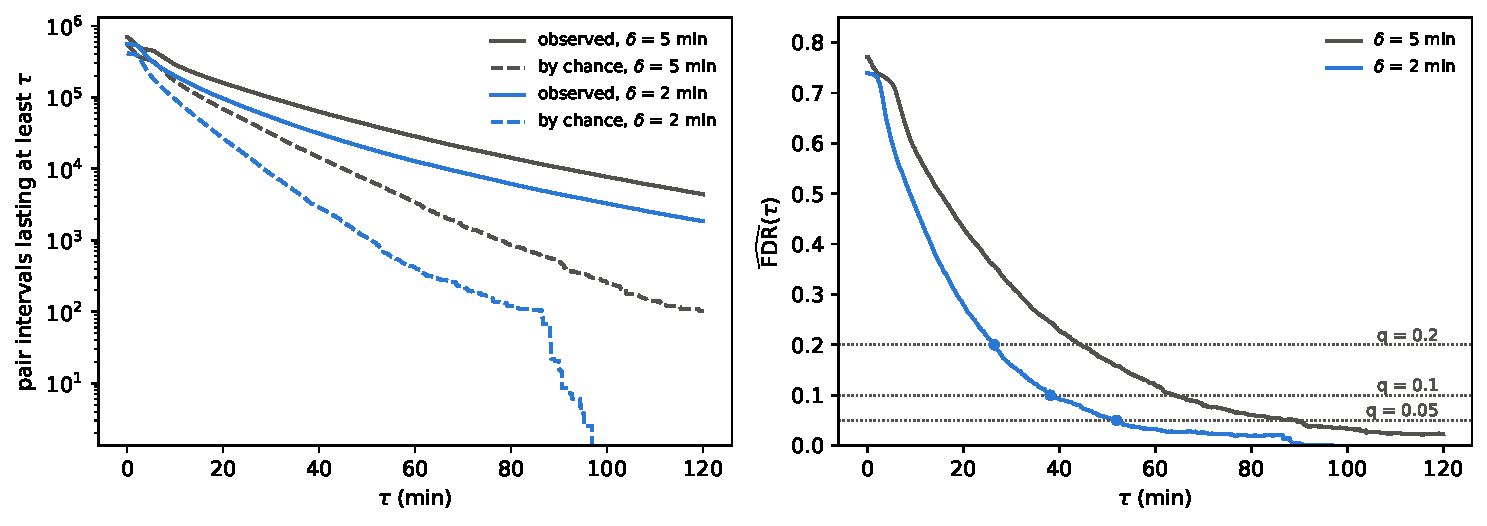
\includegraphics[width=\textwidth]{figures/assessment_fdr.pdf}
\caption{Left: real pair intervals lasting at least $\tau$ (solid) and those chance alone
gives (dashed), with $\delta=5$~min (grey) and $\delta=2$~min (blue), on the whole archive.
Right: their ratio, the false discovery rate of Eq.~\eqref{eq:fdr}; dots mark $\tau^*$ for
$q=0.05$, 0.1 and 0.2 with $\delta=2$~min.}
\label{fig:fdr}
\end{figure}

Most contacts are chance (Figure~\ref{fig:fdr}): 74\% of all pair intervals with
$\delta=2$~min (77\% with 5~min), 47\% of those lasting 10~min, 16\% of those lasting 30~min.
Short contacts say little; only long ones are mostly real. So $\tau^*$ is tens of minutes: it is
the duration at which the real contacts outnumber chance by the factor $1/q$. Resampling the dates
200 times moves $\tau^*$ by a few minutes (Table~\ref{tab:q}): the curve sets it, and the noise of
the surrogates barely moves it.

\subsection{How much the shift matters}\label{sec:shift-classes}

Does the length of the shift change what counts as chance? We recomputed the false discovery rate
with only the surrogate pairs of each date whose shift falls in one class, each class with its own
exposure $S_d$ and intervals, on the 2\,737 dates (of 6\,209) that have surrogates in every class
(Table~\ref{tab:shift-classes}).

\begin{table}
\centering
\small
\begin{tabular}{@{}l r c c c c@{}}
\toprule
Surrogates & pairs & $\widehat{\mathrm{FDR}}$(10 min) & $\widehat{\mathrm{FDR}}$(30 min) & $\tau^*$ (min) & 5--95\% over dates \\
\midrule
all shifts & 241\,824 & 0.48 & 0.16 & 38.2 & 37.0--41.5 \\
$|r|<30$ min & 69\,444 & 0.73 & 0.31 & 53.3 & 49.7--72.0 \\
$|r|\ge60$ min & 119\,687 & 0.26 & 0.05 & 23.0 & 21.1--24.4 \\
\bottomrule
\end{tabular}
\caption{The false discovery rate and $\tau^*$ ($q=0.1$, $\delta=2$~min) with the surrogates of
one class of shifts, on the 2\,737 dates with surrogates in each class.}
\label{tab:shift-classes}
\end{table}

It does, by more than a factor two. Short shifts give 2.8 times the chance of long ones at 10~min
and 5.7 times at 30~min, and $\tau^*$ goes from 23~min with shifts of an hour or more to 53~min
with shifts under 30~min; with all the shifts it is 38~min, as on the whole archive. Two effects
add up and cannot be separated here. Short shifts keep the weather of the hour, and they also
bring within $\delta$ the pilots who follow each other a few minutes apart, who are many: real
correspondences are still 2 to 3 times chance between 195 and 500~s
(Section~\ref{sec:delta-choice}).

\paragraph{What we keep.} Chance is what the same routes give without synchrony, with shifts that
follow the takeoff delays of the day. A contact counts only if it lasts at least $\tau^*$, the
duration at which at most a share $q$ of the contacts is chance; $q$ and $\delta$ are chosen in
Section~\ref{sec:tuning}.

\section{The parameters on the data}\label{sec:tuning}

The method has three kinds of parameters (Table~\ref{tab:parameters}). The \emph{tolerances} say
when two positions match: $\delta$, $\varepsilon_h$, $\varepsilon_z$, $\theta_{\max}$, $g$. The
\emph{duration} $\tau^*$ says how long a match must last to be a contact; it follows from the
share $q$ of chance contacts we accept (Section~\ref{sec:fdr}). The other \emph{settings} make the
computation exact or fast and are fixed by physical bounds. Each tolerance is compared with chance
through the null model of Section~\ref{sec:null}: the profiles of this section use a sample of
300 random dates, the choices of $\delta$ and $q$ the whole archive.

\begin{table}
\centering
\small
\begin{tabularx}{\textwidth}{@{}l l X@{}}
\toprule
Parameter & Value & How it was set \\
\midrule
$\delta$, largest delay & 2 min & measured on the delay profile, Section~\ref{sec:delta-choice} \\
$q$, accepted false discovery rate & 0.1 & trade-off, Section~\ref{sec:q} \\
$\tau^*$, shortest contact & 38.1 min & computed from $q$ and the null model, Section~\ref{sec:fdr} \\
$\varepsilon_h$, $\varepsilon_z$ & 500 m, 300 m & definitions: profiles without an edge, Section~\ref{sec:tolerances} \\
$g$, longest gap joined & 120 s & definition: gaps of real and chance contacts alike, Section~\ref{sec:tolerances} \\
$\theta_{\max}$ & 45$^\circ$ & no effect on the result, Section~\ref{sec:plateau} \\
$\Delta$, $h_{\max}$, $R_\dep$, $v_{\max}$, $R_s$, $r_{\min}$ & see Section~\ref{sec:fixed} & physical bounds and exactness \\
\bottomrule
\end{tabularx}
\caption{The parameters and how each was set.}
\label{tab:parameters}
\end{table}

\subsection{The maximum delay \texorpdfstring{$\delta$}{delta}}\label{sec:delta-choice}

Section~\ref{sec:delta} bounds $\delta$ by the visual range, at about 5~min. Here the data say
how long the delay between two pilots who fly together actually is.

\paragraph{The delay profile.} For every delay $l$, the correspondences $(t,t+l)$ of the real
pairs and of the surrogate pairs were counted, per second of exposure, with a window of 15~min on
300 random dates (58\,910~h of real exposure):
\begin{equation}\label{eq:profile}
  R(l)=\frac{\text{real correspondences at delay } l \text{ per second of exposure}}
             {\text{chance correspondences at delay } l \text{ per second of exposure}} .
\end{equation}
Chance is flat in the delay, as it should: a shifted copy has no preferred delay. The real
pairs peak at a few seconds, where they have 5.6 times the correspondences of chance, and
decay: $R$ falls below 4 at 105~s, below 3 at 195~s and below 2 at 500~s, and is still 1.5 at
15~min (Figure~\ref{fig:delays}). The excess has two parts. The fast one, within 2--3~min, is
pilots flying together. The slow one, which has not ended at 15~min, is pilots who use the
same thermals at about the same time without following each other, a synchrony that the
shifts of the surrogates remove. A rule such as ``the delay that holds 95\% of the excess''
would pick 13~min, because it counts the slow tail; that is why we read the ratio instead.

\begin{figure}
\centering
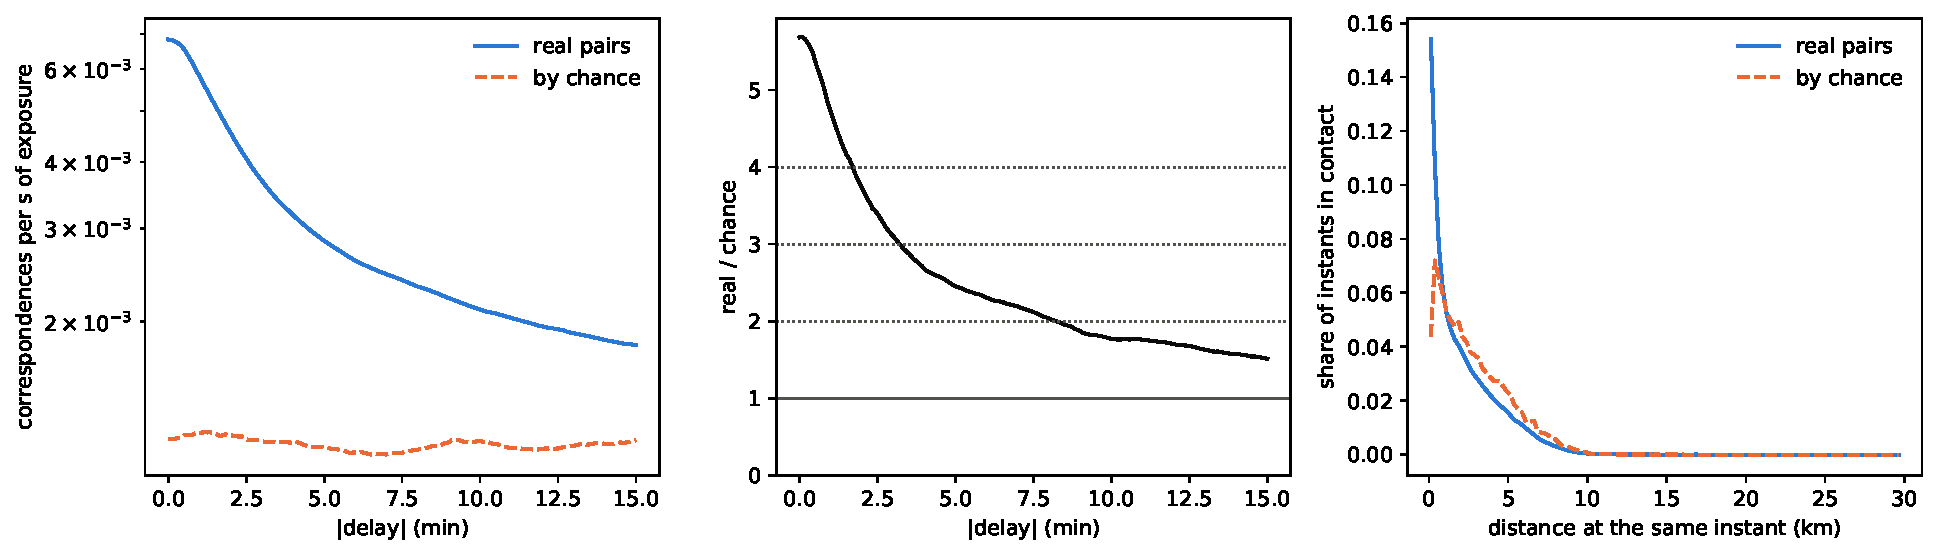
\includegraphics[width=\textwidth]{figures/assessment_delays.pdf}
\caption{The delay profile on 300 dates with a 15~min window. Left: correspondences per
second of exposure at each delay, real and by chance. Middle: their ratio $R(l)$ of
Eq.~\eqref{eq:profile}, with the levels 4, 3 and 2. Right: the distance between the two
pilots at the same instant when one is on the path of the other.}
\label{fig:delays}
\end{figure}

\paragraph{The delay inside the contacts.} The profile counts correspondences; this view looks at
the contacts themselves, through the delay $\ell_{\rm med}$ of each pair interval
(Section~\ref{sec:lag}). Its absolute value was computed for every pair interval of the run with
$\delta=5$~min, whose window is wide enough to show where the delays fall: 965\,770 intervals, of
which 169\,517 have all their instants in search and no delay.

\begin{table}
\centering
\small
\begin{tabular}{@{}l r c c c@{}}
\toprule
Duration of the interval & intervals & median $|\ell_{\rm med}|$ & within 2 min & at the edge \\
\midrule
under 10 min & 436\,575 & 210 s & 32\% & 29\% \\
10--30 min & 246\,587 & 160 s & 39\% & 12\% \\
30--90 min & 102\,357 & 80 s & 64\% & 2.1\% \\
90 min or more & 10\,734 & 25 s & 90\% & 6 intervals \\
\bottomrule
\end{tabular}
\caption{The delay of the pair intervals by their duration ($\delta=5$~min, whole archive). At
the edge: $|\ell_{\rm med}|\ge285$~s, the last 15~s of the window.}
\label{tab:ell}
\end{table}

\begin{figure}
\centering
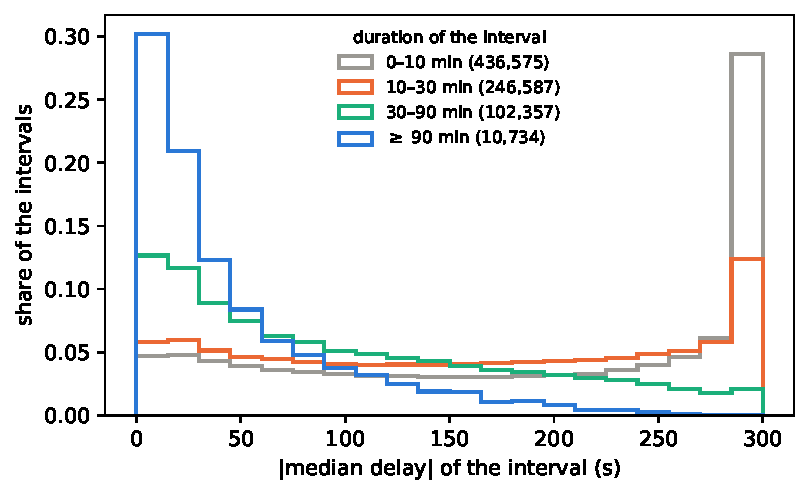
\includegraphics[width=0.62\textwidth]{figures/assessment_ell.pdf}
\caption{Distribution of the $|\ell_{\rm med}|$ of the pair intervals, by their duration
($\delta=5$~min, whole archive).}
\label{fig:ell}
\end{figure}

The longer the contact, the shorter the delay (Table~\ref{tab:ell}, Figure~\ref{fig:ell}). A
pair that only shares route and weather matches at any delay of the window, and its closest
correspondence is often at the largest ones: short intervals pile up at the edge, 29\% of
those under 10~min. The contacts of at least 90~min, all above $\tau^*$ of this run
(89.5~min), have a median delay of 25~s; 90\% of them lie within 2~min and only 6 of 10\,734
at the edge. Long contacts are pilots a few tens of seconds apart on the same path.

\paragraph{Choice.} We take $\delta=2$~min: within it the real correspondences are at least 3.7
times chance, and it contains nine in ten of the long contacts. Shortening the delay also
shortens $\tau^*$, since fewer chance matches enter: from 89.5 to 51.9~min at $q=0.05$
(Table~\ref{tab:q}).

\paragraph{Distance at the same instant.} The delay also bounds how far apart two pilots in
contact can be at the same instant: at most
$\varepsilon_h+v_{\max}\delta\approx0.5+27.8\times120/1000\approx3.8$~km. A separation of 6~km,
the largest we want to call a group, is never reached by one pair; a group, a chain of pairs, can
be wider. Even with the 15~min window, 58\% of the instants in contact have the two pilots within
2~km and 94\% within 6~km (Figure~\ref{fig:delays}, right).

The same distance was also counted without requiring a correspondence: at every grid instant when
both fly after departure, for all the real pairs and for the surrogates, on the dates of
Figure~\ref{fig:delays} that have surrogates (210 of 300, 58\,901~h of real exposure). Real pairs
are much closer than chance at short distance and have no edge (Figure~\ref{fig:separation}):
the ratio $g(d)$ is 10.4 within 100~m, below 2 from 500~m, below 1.5 from 900~m, below 1.1 from
2.7~km and below 1 from 5.7~km. Real pairs spend 6.6\% of their time together within 1~km of each
other, against 2.8\% by chance. Beyond 6~km $g$ falls slightly below 1, because both distributions
sum to one. The excess reaches several kilometres, beyond the visual range of 1.5~km of
Section~\ref{sec:delta}. Since the surrogates also change the hour, this excess may hold the
weather of the hour as well as sight, so it bounds neither the visual range nor the range of
following.

\begin{figure}
\centering
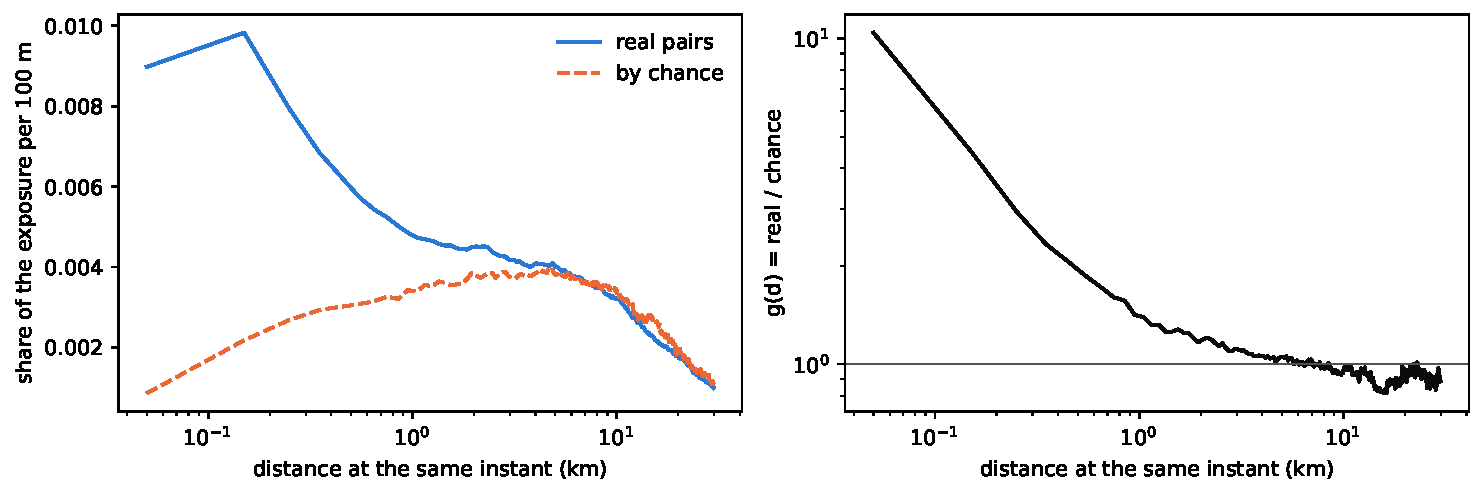
\includegraphics[width=\textwidth]{figures/assessment_separation.pdf}
\caption{Distance between the two pilots at the same instant, over all the time both fly, on
210 dates. Left: share of the exposure in each 100~m bin, real pairs and chance. Right: their
ratio $g(d)$.}
\label{fig:separation}
\end{figure}

\subsection{The tolerances against chance}\label{sec:tolerances}

In analogy with the delay profile, with $\delta=2$~min and the null model of the chosen run, at
every instant $t$ of pilot $i$ on the 210 dates of Figure~\ref{fig:separation}:
\begin{itemize}
\item the smallest horizontal distance between $i$ at $t$ and $j$ at $t+l$, $|l|\le\delta$,
  over the delays with $|z_i(t)-z_j(t+l)|<\varepsilon_z$ and headings that pass (left of
  Figure~\ref{fig:tolerances});
\item the smallest height difference over the delays with horizontal distance
  $<\varepsilon_h$ and headings that pass (middle);
\item the gaps between consecutive instants of contact of a pair (right).
\end{itemize}

\begin{figure}
\centering
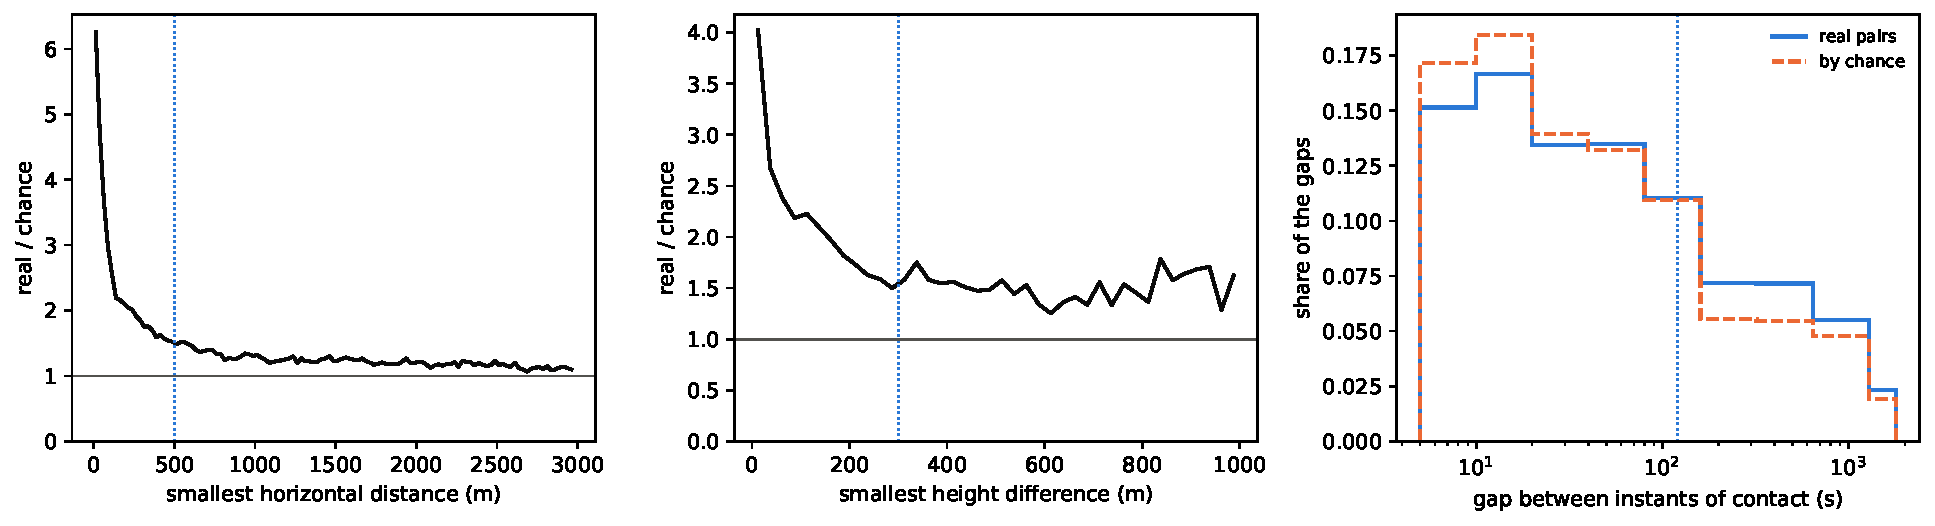
\includegraphics[width=\textwidth]{figures/assessment_tolerances.pdf}
\caption{The tolerance profiles on 210 dates. Left and middle: real pairs over chance, per
second of exposure, by the smallest horizontal distance and the smallest height difference to
the path of the other pilot within $\delta$; dotted, the values in use. Right: the lengths of
the gaps between instants of contact, as a share of all gaps (the 8\% of real and 9\% of chance
gaps longer than 30~min are not drawn); dotted, $g$.}
\label{fig:tolerances}
\end{figure}

None of the three has an edge (Figure~\ref{fig:tolerances}). The horizontal ratio is 6.3 within
25~m, below 2 from 250~m, below 1.5 from 500~m, and still 1.13 between 2.5 and 3~km. The
vertical ratio is 4.0 within 25~m and below 2 from 150~m; from 275~m on it stays near 1.5
(1.51 on average up to 1~km), the excess that the horizontal condition alone gives. Both values
in use sit where real pairs are about 1.5 times chance.

Real pairs have 1.46 times the gaps of chance per hour, because they have more contact, but the
lengths of the gaps are the same: the shares of each class differ by at most 2 points. The
gaps come from how pilots fly in and out of each other's path, the same in real and in chance
contacts, so the data do not single out $g$.

\subsection{One parameter at a time}\label{sec:plateau}

A plateau is a range of values of the tolerances around which the result does not change: a
value inside it makes the result insensitive to the exact threshold. If there is none, the
thresholds decide the result, and this must be said. The result is measured by $f_G$, the
fraction of the flight time after the departure spent in a group:
\begin{equation}\label{eq:fg}
  f_G=\frac{\sum_i\bigl|\{t\in T^\dep_i:\ \gamma_i(t)\notin\{\st{L},\st{S}\}\}\bigr|}{\sum_i|T^\dep_i|}.
\end{equation}
We changed one parameter at a time on 300 random dates, recalibrating $\tau^*$ each time, with
$\delta=5$~min (Table~\ref{tab:plateau}). $\theta_{\max}$ changes nothing: contacts in glide are
few. The others move $f_G$ by up to a factor three, mostly through $\tau^*$: there is no plateau,
in agreement with the profiles, and $\varepsilon_h$, $\varepsilon_z$ and $g$ are definitions. On
300 dates $\tau^*$ is noisy (126~min with the starting values against 89.5 on the whole archive,
and six settings stop at the same surrogate interval); a conclusive check needs the whole archive
for each setting, about one hour each. It was not repeated with $\delta=2$~min.

\begin{table}
\centering
\small
\begin{tabular}{@{}l c c c c@{}}
\toprule
Setting ($\delta=5$ min unless stated) & $\tau^*$ (min) & $f_G$ & episodes & flights in a group \\
\midrule
starting values & 126.1 & 0.034 & 98 & 210 \\
$\varepsilon_h=250$ m & 75.1 & 0.058 & 253 & 537 \\
$\varepsilon_h=1000$ m & 126.8 & 0.065 & 162 & 372 \\
$\varepsilon_z=150$ m & 126.1 & 0.020 & 61 & 125 \\
$\varepsilon_z=600$ m & 126.1 & 0.044 & 122 & 268 \\
$\delta=2$ min & 42.6 & 0.106 & 600 & 1\,170 \\
$\delta=10$ min & 128.4 & 0.062 & 153 & 365 \\
$\theta_{\max}=30^\circ$ & 126.1 & 0.034 & 97 & 208 \\
$\theta_{\max}=90^\circ$ & 126.1 & 0.034 & 98 & 210 \\
$g=60$ s & 75.8 & 0.087 & 332 & 732 \\
$g=300$ s & 126.1 & 0.055 & 141 & 318 \\
\bottomrule
\end{tabular}
\caption{One parameter at a time on 300 random dates (7\,051 flights), $q=0.05$.}
\label{tab:plateau}
\end{table}

\subsection{The false discovery rate \texorpdfstring{$q$}{q}}\label{sec:q}

$q$ is the share of chance contacts we accept among those we keep. A smaller $q$ keeps only
very long contacts and few groups, all of them real; a larger $q$ sees more groups, with more
chance among them. Table~\ref{tab:q} and Figure~\ref{fig:q} give the trade-off.

\begin{table}
\centering
\small
\begin{tabular}{@{}l l c c c c c@{}}
\toprule
$\delta$ & $q$ & $\tau^*$ (min) & 5--95\% over dates & para in a group & hang in a group & episodes \\
\midrule
5 min & 0.05 & 89.5 & 79.5--91.5 & 8.9\% & 2.1\% & 6\,090 \\
2 min & 0.05 & 51.9 & 49.1--53.3 & 13.7\% & 3.8\% & 10\,553 \\
2 min & 0.1  & 38.1 & 37.0--41.1 & 21.7\% & 6.9\% & 17\,169 \\
2 min & 0.2  & 26.4 & 25.2--27.2 & 31.7\% & 13.9\% & 26\,504 \\
\bottomrule
\end{tabular}
\caption{$\tau^*$ and the groups it gives. Flights with a logger of at most 10~s and a
position after departure: 154\,598 paragliders and 6\,039 hang gliders.}
\label{tab:q}
\end{table}

\begin{figure}
\centering
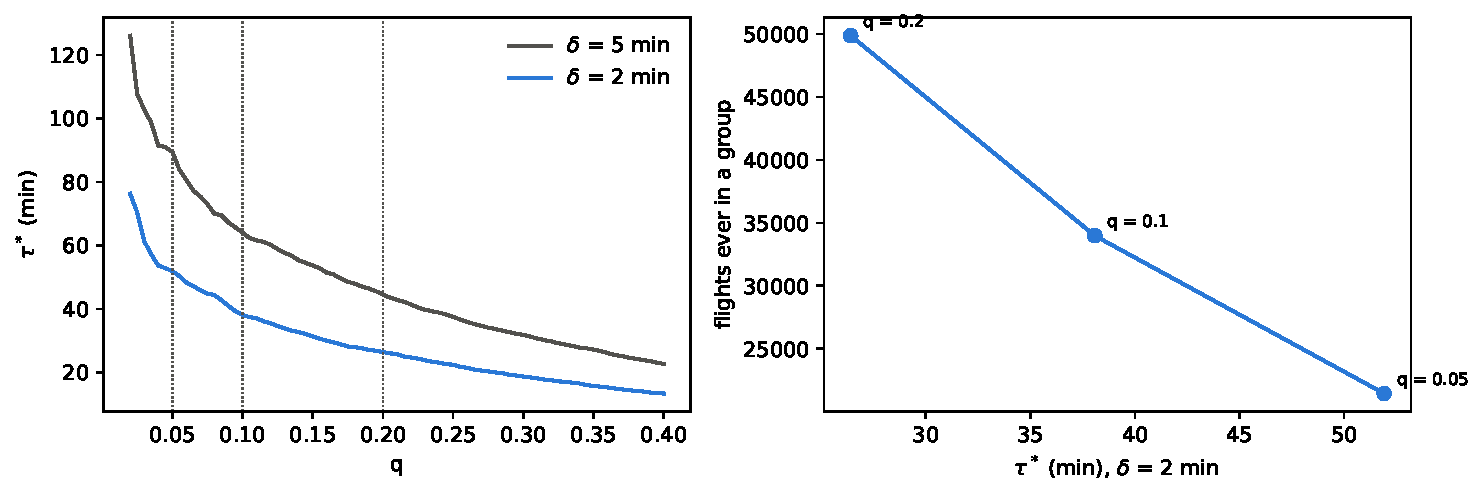
\includegraphics[width=\textwidth]{figures/assessment_q.pdf}
\caption{Left: $\tau^*$ as a function of $q$, for the two delays. Right: flights ever in a
group against $\tau^*$, for $q=0.05$, 0.1 and 0.2 with $\delta=2$~min.}
\label{fig:q}
\end{figure}

We take $q=0.1$: at most one contact in ten is chance, and $\tau^*=38.1$~min. Going to 0.2 would
lower $\tau^*$ to 26~min but would let chance make one group in five.

\subsection{Fixed settings}\label{sec:fixed}

\begin{itemize}
\item $\Delta=5$~s, the common grid: a pilot is at most 69~m from a grid position at
  100~km/h, against $\varepsilon_h=500$~m (Section~\ref{sec:phase0}).
\item $h_{\max}=10$~s: positions are interpolated only between fixes at most 10~s apart; the
  flights of coarser loggers are left out of the statistics.
\item $R_\dep=3$~km: contacts around the takeoff, before the first exit from this disc, are not
  counted (Section~\ref{sec:local}).
\item $v_{\max}=100$~km/h, the speed of the candidate filter: pieces of track end at every
  faster step, so the filter never misses a correspondence (Lemma~\ref{lem:filter}, checked
  against every pair of instants on synthetic days). The profiles of
  Section~\ref{sec:tolerances} widen the filter to 3~km, the largest distance they count.
\item $R_s=10$~km, $r_{\min}=2\delta+\Delta$, at most 200 surrogate pairs per date: the null
  model of Section~\ref{sec:null}.
\end{itemize}

\section{The groups on the archive}\label{sec:structure}

With the chosen values, $\delta=2$~min and $q=0.1$, 21.7\% of the paraglider flights and 6.9\% of
the hang-glider flights fly in a group at some point, in 17\,169 episodes (Table~\ref{tab:q}).
This section describes those groups: their sizes and durations, how they change, and where in the
flight and when in the day they form. Section~\ref{sec:group-structure} asks what holds them
together. Bands are 5--95\% of 200 draws of the dependency blocks, or of the dates where the
captions say so.

\subsection{Sizes and durations}\label{sec:sizes}

A configuration is a group with fixed members; it ends when a member joins or leaves. Its
duration runs from its start to its end, and its participants are its members at once. An episode
is a chain of configurations; its duration runs from the start of its first configuration to the
end of its last, and its participants are the distinct flights it holds. The participants are
counted in two ways: the share of the episodes (or configurations) of each size, and the share of
their total duration.

\begin{figure}
\centering
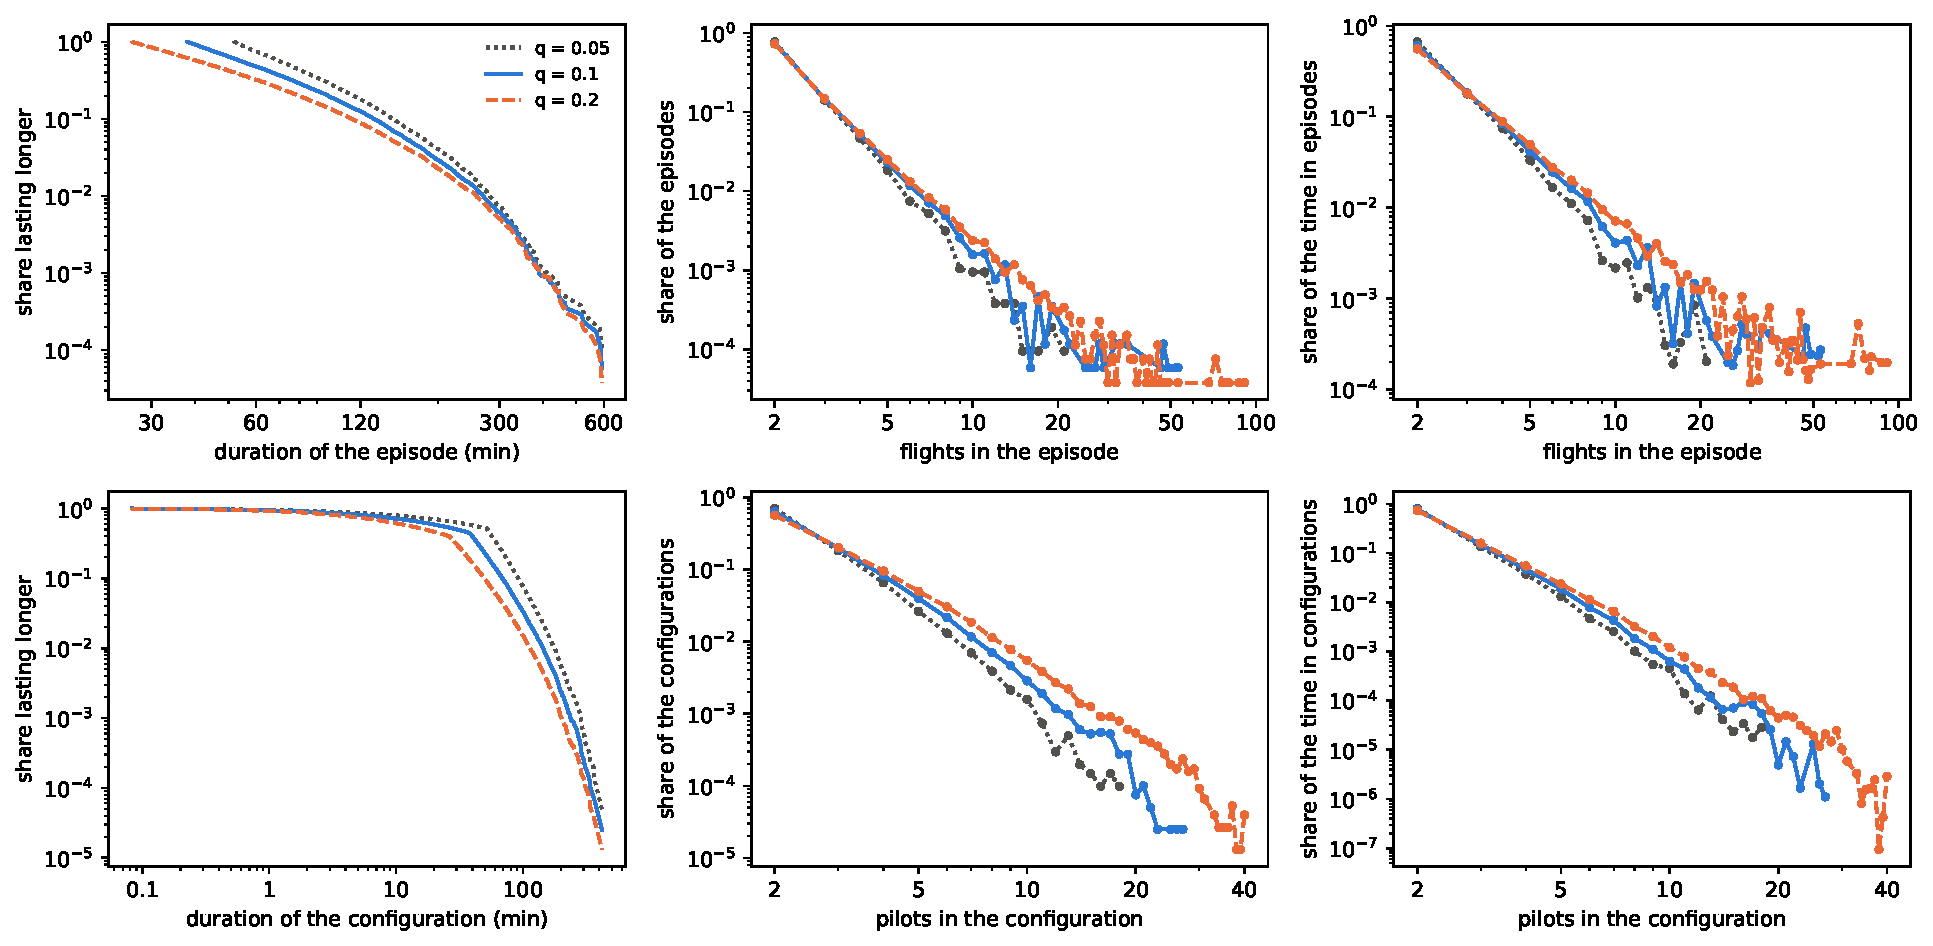
\includegraphics[width=\textwidth]{figures/assessment_structure.pdf}
\caption{Episodes (top) and configurations (bottom), $\delta=2$~min, whole archive, for three
values of $q$. Left: share lasting longer than a duration. Middle: share of each size. Right:
share of the total duration in each size.}
\label{fig:structure}
\end{figure}

\begin{table}
\centering
\small
\begin{tabular}{@{}l l r r c c c c r@{}}
\toprule
& $q$ & number & median & \multicolumn{2}{c}{2 participants} & \multicolumn{2}{c}{5 or more} & largest \\
& & & duration & items & time & items & time & \\
\midrule
episodes & 0.05 & 10\,553 & 74.6 min & 77\% & 67\% & 3.9\% & 8.1\% & 21 \\
 & 0.1 & 17\,169 & 58.2 min & 74\% & 61\% & 5.7\% & 12.6\% & 53 \\
 & 0.2 & 26\,504 & 44.5 min & 73\% & 56\% & 7.0\% & 17.2\% & 91 \\
\midrule
configurations & 0.05 & 20\,275 & 52.7 min & 70\% & 81\% & 5.6\% & 2.3\% & 18 \\
 & 0.1 & 40\,051 & 30.4 min & 63\% & 77\% & 9.4\% & 3.5\% & 27 \\
 & 0.2 & 75\,953 & 17.1 min & 56\% & 74\% & 14.1\% & 5.0\% & 40 \\
\bottomrule
\end{tabular}
\caption{Episodes and configurations for three values of $q$ ($\delta=2$~min). Items: share of
the episodes or configurations of that size; time: share of their total duration.}
\label{tab:structure}
\end{table}

With the chosen values the median episode lasts 58.2~min and three in four are pairs
(Table~\ref{tab:structure}). Episodes last at least $\tau^*$, since a contact must. Weighted by
duration the pairs weigh less, 61\% of the episode time, because larger episodes last longer:
those of five flights or more are 5.7\% of the episodes and 12.6\% of their time.

Configurations have no minimum duration: every arrival or departure of a member starts a new
one, so 10\% last less than 2.1~min, and the median is 30.4~min. Weighted by duration the pairs
weigh more, 77\% of the time against 63\% of the configurations, because large configurations
change quickly. \StWithHang\% of the configurations hold a hang glider.

A larger $q$, hence a shorter $\tau^*$, gives more and shorter groups, and larger ones: the
largest episode holds 21 flights with $q=0.05$, 53 with 0.1 and 91 with 0.2. The shares of the
small sizes change little; the tail moves.

\subsection{How configurations change}\label{sec:describe}

A configuration ends in one of five ways: a \emph{join} (members added), a \emph{leave} (members
removed in flight), a \emph{landing} (a removed member lands within 5~s, the grid step), a
\emph{split} (into several configurations) or a \emph{merge} (with others, into one); a
configuration of two pilots that loses one ends the group. Each ending is one component of a
bipartite graph between the configurations that end and those that start at one instant
(Appendix~\ref{app:graphs}). The rates are configurations ending per hour spent at each size
(Table~\ref{tab:rates}).

\begin{table}
\centering
\footnotesize
\begin{tabular}{@{}r r r l l l l l@{}}
\toprule
pilots & hours & median (min) & join & leave & landing & split & merge \\
\midrule
2 & 17\,389 & 41 & 0.31\,{\tiny[0.30, 0.32]} & 0.96\,{\tiny[0.95, 0.97]} & 0.098\,{\tiny[0.094, 0.10]} & -- & 0.085\,{\tiny[0.079, 0.092]} \\
3 & 3\,349 & 20 & 0.54\,{\tiny[0.52, 0.57]} & 1.6\,{\tiny[1.6, 1.6]} & 0.050\,{\tiny[0.044, 0.056]} & -- & 0.16\,{\tiny[0.15, 0.18]} \\
4 & 1\,059 & 13 & 0.70\,{\tiny[0.66, 0.76]} & 1.6\,{\tiny[1.6, 1.7]} & 0.042\,{\tiny[0.032, 0.051]} & 0.48\,{\tiny[0.45, 0.52]} & 0.26\,{\tiny[0.22, 0.29]} \\
5 & 421 & 11 & 0.88\,{\tiny[0.80, 0.96]} & 1.7\,{\tiny[1.6, 1.8]} & 0.036\,{\tiny[0.021, 0.057]} & 0.82\,{\tiny[0.76, 0.88]} & 0.32\,{\tiny[0.26, 0.37]} \\
6 & 176 & 8 & 1.1\,{\tiny[0.93, 1.2]} & 2.1\,{\tiny[1.9, 2.3]} & 0.028\,{\tiny[0.011, 0.048]} & 1.2\,{\tiny[1.0, 1.3]} & 0.51\,{\tiny[0.40, 0.63]} \\
7 & 96 & 7 & 1.1\,{\tiny[0.91, 1.3]} & 2.0\,{\tiny[1.8, 2.2]} & 0.031\,{\tiny[0.0089, 0.074]} & 1.3\,{\tiny[1.1, 1.5]} & 0.40\,{\tiny[0.30, 0.53]} \\
8+ & 107 & 4 & 1.8\,{\tiny[1.5, 2.2]} & 2.5\,{\tiny[2.2, 2.8]} & 0.028\,{\tiny[0.0084, 0.057]} & 2.7\,{\tiny[2.4, 3.1]} & 1.0\,{\tiny[0.73, 1.2]} \\
\bottomrule
\end{tabular}

\caption{By size: hours spent, median duration of a configuration, and configurations ending per
hour by outcome, with 5--95\% bands.}
\label{tab:rates}
\end{table}

\begin{itemize}
  \item \textbf{Most episodes never change:} \StEpisodeSingle\% of the \StEpisodes{} episodes are one
        configuration; \StEpisodeSplit\% hold a split, \StEpisodeMerge\% a merge.
  \item \textbf{The episode lasts, the configuration does not.} \StEpisodeTwoHours\% of the episodes
        last 2~h or more. A configuration lasts \StMedianConfTwo~min with 2 pilots and
        \StMedianConfMax~min with \StSizeMax{} or more: joins, leaves, splits and merges all grow with
        size, so a large configuration changes members every few minutes.
  \item \textbf{Groups break in flight:} \StEndFlight\% of the \StEnds{} configurations that end a group
        do so in flight, \StEndLanding\% at a landing. \StFormDeparture\% of the \StFormations{}
        configurations with no predecessor form when a member departs: pilots who took off together.
  \item \textbf{A pair} ends \StRateLeaveTwo{} times per hour because the two separate, \StRateJoinTwo{}
        because a third pilot joins, \StRateMergeTwo{} by a merge and \StRateLandingTwo{} by a landing.
\end{itemize}

\subsection{Where in the flight groups form and break}\label{sec:phases}

On 1~Hz flights, where the phases are labelled: the phase at the instant a flight enters
(\Entries{}) or leaves (\Exits{}) a group, against the shares of time in each phase; entries at the
departure (\AtDeparture{}) and exits at the landing (\AtLanding{}) are counted apart
(Figure~\ref{fig:phases}, Table~\ref{tab:phases}).

\begin{figure}
\centering
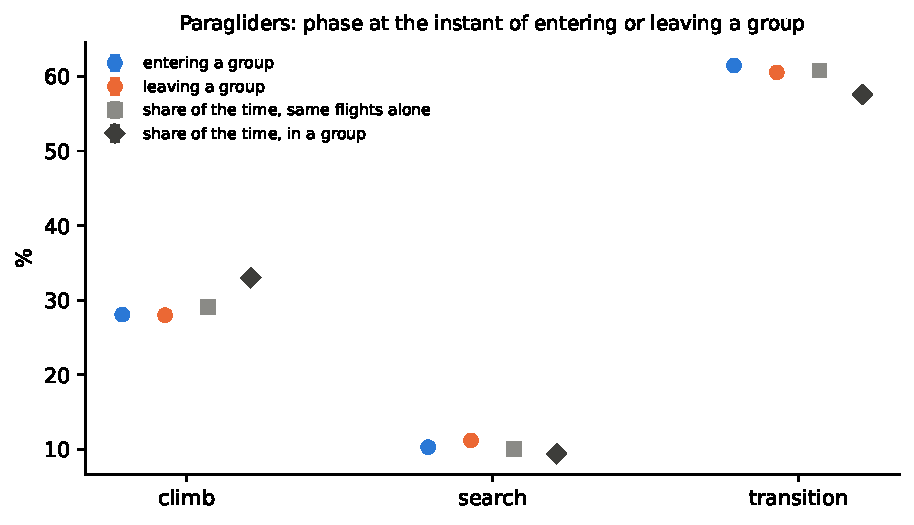
\includegraphics[width=0.55\textwidth]{figures/structure/mechanisms_phases.pdf}
\caption{Phase at entry and exit, against the time shares (bands: blocks).}
\label{fig:phases}
\end{figure}

\begin{table}
\centering
\footnotesize
\begin{tabular}{@{}l l l l@{}}
\toprule
 & climb (\%) & search (\%) & transition (\%) \\
\midrule
entering a group & 28.1 [27.6, 28.5] & 10.3 [10.0, 10.6] & 61.5 [61.0, 61.9] \\
leaving a group & 28.0 [27.6, 28.3] & 11.2 [10.9, 11.5] & 60.6 [60.1, 61.0] \\
share of time, alone & 29.1 [28.9, 29.3] & 10.1 [10.0, 10.2] & 60.8 [60.6, 61.0] \\
share of time, in a group & 33.0 [32.8, 33.2] & 9.4 [9.2, 9.6] & 57.6 [57.3, 57.9] \\
\bottomrule
\end{tabular}

\caption{Phase at the instant of entering or leaving a group, and shares of time in each phase
(percent, with 5--95\% bands; 1~Hz flights).}
\label{tab:phases}
\end{table}

Entries fall in climbs \PhaseEntryClimb\%, searches \PhaseEntrySearch\% and glides
\PhaseEntryTransition\% of the cases, exits \PhaseExitClimb, \PhaseExitSearch, \PhaseExitTransition\%,
against \PhaseAloneClimb, \PhaseAloneSearch, \PhaseAloneTransition\% of the time alone: there is no
phase where groups preferentially form or break. \EntriesEarly\% of the entries are within 10~min of
the departure.

\subsection{When in the day}\label{sec:hours}

\begin{figure}
\centering
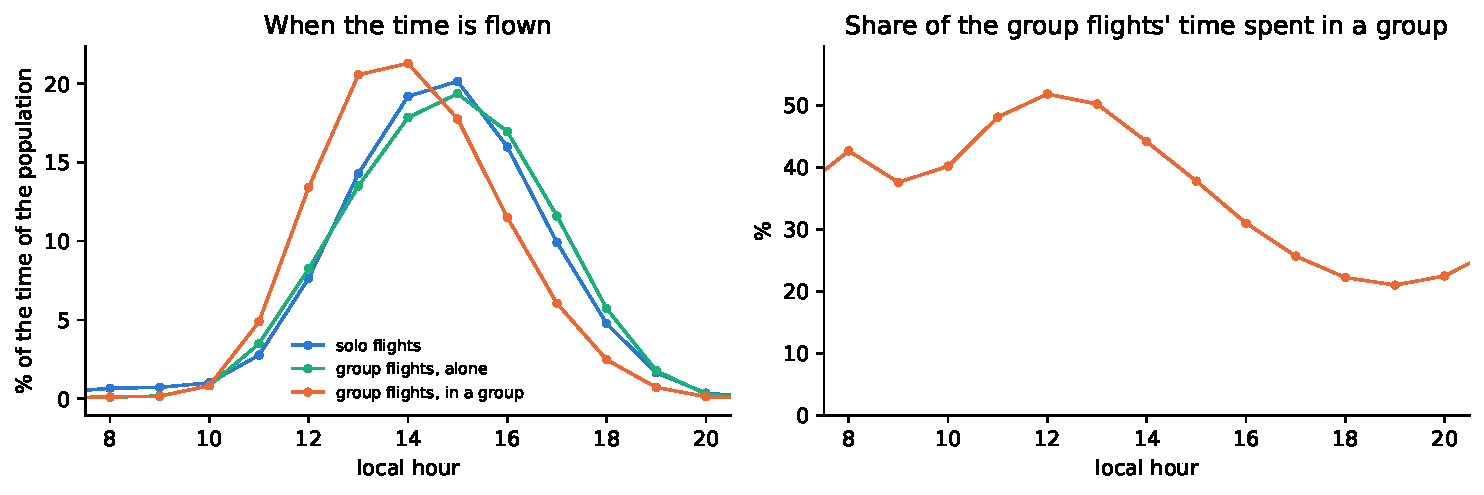
\includegraphics[width=0.9\textwidth]{figures/structure/mechanisms_hours.pdf}
\caption{Time of solo flights (S), of group flights alone (A) and in a group (G) over the local hour
(left), and the share of a group flight's time spent in a group (right).}
\label{fig:hours}
\end{figure}

Group time is concentrated around midday: \GroupShareNoon\% of a group flight's time at
\GroupShareNoonHour~h, \GroupShareMorning\% at 9~h, \GroupShareEvening\% at 18~h
(Figure~\ref{fig:hours}).

\section{Use and limits}\label{sec:use-limits}

What are the labels for, and what must the thesis declare when it uses them? They exist to compare
how pilots move in a group and alone; this section says how, which choices come with them, and
what has been checked.

\subsection{Comparing group and solo flight}\label{sec:comparison}

\paragraph{Labels on the phases.} For a run $\sigma$ of one phase (climb, search or glide) of
flight $i$, with interval $J_\sigma$, we define the fraction in a group and the mean size:
\begin{equation}\label{eq:segment}
  f_\sigma=\frac{\bigl|\{t\in J_\sigma\cap T^\dep_i:\ \gamma_i(t)\notin\{\st{L},\st{S}\}\}\bigr|}{|J_\sigma\cap T^\dep_i|},
  \qquad
  \bar n_\sigma=\text{mean of } n_i(t) \text{ over } J_\sigma\cap T^\dep_i ,
\end{equation}
with $n_i(t)$ the number of members of the group of $i$ at $t$, 1 if solo. The run is
\emph{in a group} if $f_\sigma\ge1/2$ and \emph{solo} if $f_\sigma=0$; the intermediate cases are
excluded, or $f_\sigma$ is used as a continuous covariate (Figure~\ref{fig:segments}). Runs in the
local phase are excluded.

\begin{figure}
\centering
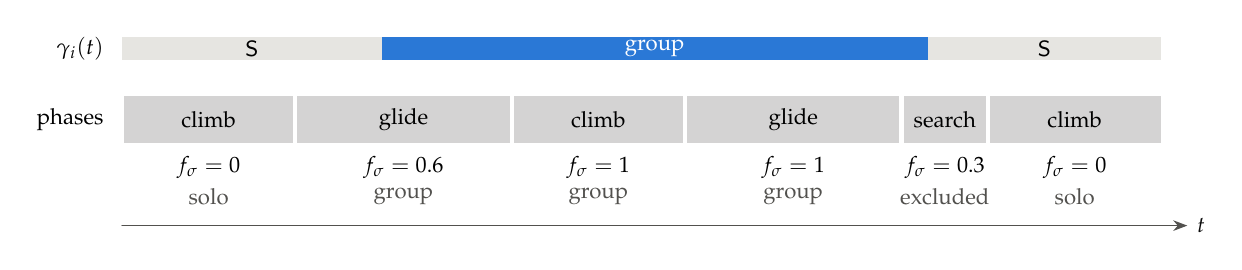
\begin{tikzpicture}[x=1.1cm,y=1cm,
    seg/.style={draw=white, line width=1pt, minimum height=6mm, inner sep=0pt, font=\footnotesize}]
  \node[lbl, anchor=east] at (-0.1,1.2) {$\gamma_i(t)$};
  \fill[light] (0,1.05) rectangle (3.0,1.35);
  \fill[blueI] (3.0,1.05) rectangle (9.3,1.35);
  \fill[light] (9.3,1.05) rectangle (12,1.35);
  \node[font=\footnotesize] at (1.5,1.2) {\st{S}};
  \node[font=\footnotesize, text=white] at (6.15,1.2) {group};
  \node[font=\footnotesize] at (10.65,1.2) {\st{S}};
  \node[lbl, anchor=east] at (-0.1,0.3) {phases};
  \foreach \a/\b/\name/\f/\cls in {0/2/climb/0/solo, 2/4.5/glide/0.6/group, 4.5/6.5/climb/1/group,
                                   6.5/9/glide/1/group, 9/10/search/0.3/excluded, 10/12/climb/0/solo} {
    \fill[ink2!25] (\a,0.0) rectangle (\b,0.6);
    \draw[white, line width=1.5pt] (\a,0) -- (\a,0.6);
    \node[font=\footnotesize] at ({(\a+\b)/2},0.3) {\name};
    \node[font=\footnotesize, anchor=north] at ({(\a+\b)/2},-0.05) {$f_\sigma=\f$};
    \node[font=\footnotesize, anchor=north, text=ink2] at ({(\a+\b)/2},-0.45) {\cls};
  }
  \draw[->, ink2] (0,-1.05) -- (12.3,-1.05) node[right, lbl, ink] {$t$};
\end{tikzpicture}
\caption{Labels on the phases of one flight: each run of one phase gets the fraction $f_\sigma$ of
its duration spent in a group, and from it a class.}
\label{fig:segments}
\end{figure}

\paragraph{Stratification.} Group flights concentrate on the good days, at the busy sites and
around midday (Section~\ref{sec:hours}), so a global comparison would mix the effect of the group
with that of the weather. We compare within strata $s$ (date and area):
\begin{equation}\label{eq:strata}
  \hat\Delta=\sum_s w_s\bigl(\hat\theta_{G,s}-\hat\theta_{S,s}\bigr),
\end{equation}
where $\hat\theta$ is the statistic of interest and the weights $w_s$ are proportional, for
example, to the number of group runs of the stratum.

\paragraph{Uncertainties.} Runs of the same flight are not independent, and neither are those of
pilots of the same episode. The bootstrap resamples the dependency blocks (Section~\ref{sec:blocks})
within the strata.

\paragraph{Confounders.} Competition days; the level of the pilot (the same pilots often fly
together, Section~\ref{sec:partners}); the glider class (EN A--D); the time of day.

\paragraph{Questions to ask.} Distributions of the times spent in thermals and of the lengths of
the glides, in a group and alone; mean squared displacement and effective exponent; differences
between followers and leaders, by the sign of $\ell_{\rm med}$. In birds, followers leave the
thermals earlier and lower~\cite{flack2018}, and individuals with social information glide
faster~\cite{williams2018}: these are hypotheses to test on pilots before assuming them.

\subsection{Choices to declare and limits}\label{sec:parameters}

The starting values and those chosen on the data are in Table~\ref{tab:notation}. The thesis
should state these choices, each argued in the section given:
\begin{itemize}
  \item $\varepsilon_z$ encodes the notion of ``together'': shared thermals if tight, visual
        contact if wide (Section~\ref{sec:delta});
  \item $\delta$ is bounded by the visual range through $v_\xc$ (Section~\ref{sec:delta}) and
        measured on the data at 2~min; $q=0.1$ lets at most one contact in ten be chance;
        $\varepsilon_h$, $\varepsilon_z$ and $g$ show no plateau and are definitions
        (Section~\ref{sec:tuning});
  \item headings are compared only when both pilots glide; climb, search and unclassified fixes
        turn the condition off (Section~\ref{sec:roles}); \fix{in the run reported here the phases
        are Vilpellet's, on 1~Hz flights only, so the condition acts only between two such
        flights (Section~\ref{sec:data});}
  \item contacts before the departure are ignored: a group formed on the takeoff is recognised
        only after the exit from $R_\dep$ (Section~\ref{sec:local});
  \item grid positions are interpolated across at most $h_{\max}$, so tracks logged more coarsely
        enter with gaps (Appendix~\ref{sec:phase0});
  \item the signed median delay leaves out the instants of search, where the delay is not
        determined (Appendix~\ref{sec:lag});
  \item chance is defined by the null model, whose shifts of about an hour also remove the
        synchrony of pilots with the weather of the hour: what it calls real includes pilots in the
        same thermals at the same time who do not follow each other, the ``same air'' notion of
        Remark~\ref{rem:notions}, which is no proof of interaction; $\tau^*$ is 23~min with shifts
        over an hour and 53~min with shifts under 30~min (Section~\ref{sec:shift-classes});
  \item the errors of the phase labelling reach the heading condition: a climb labelled as glide
        compares headings that turn, and joining the short gaps mitigates the problem.
\end{itemize}
The measurements have three further limits:
\begin{itemize}
  \item the profiles of Sections~\ref{sec:delta-choice} and~\ref{sec:tolerances} are on one sample
        of 300 dates;
  \item the plateau check of Section~\ref{sec:plateau} is on 300 dates and with the starting delay
        of 5~min;
  \item the data are the cleaned tracks of the old repository (soaring, tag
        \texttt{legacy-final}), not the pre-processing of xc-dynamics that
        Section~\ref{sec:data} describes.
\end{itemize}

\subsection{Checks done}\label{sec:checks-done}

\begin{itemize}
  \item \textbf{Code against this note.} Every phase was compared with its code (grid, departure,
        candidate filter, scan of delays, contact, gaps, signed delay, null model, groups,
        episodes, membership, blocks): all implemented as written, with four differences of text,
        now corrected in red: (1) the phases of the run are Vilpellet's, on 1~Hz flights, so the
        heading condition acts only between two such flights; (2) headings are in the east and
        north of the first fix of each flight, not of the fix itself; (3) a contact is kept only
        from the later departure to the earlier landing; (4) instants in a gap of the track are
        labelled solo in the tables.
  \item \textbf{Properties of the tables} of the chosen run: every pair interval lasts at least
        $\tau^*=2285$~s and lies where both flights fly after departure; every group has at
        least two members; membership covers each flight from takeoff to landing without holes; on
        3\,000 flights the group time equals the union of its pair intervals; on 3\,000
        groups the members are connected at the midpoint and no active interval leaves; on
        2\,000 episodes every group but the first starts when another ends and shares a
        member; the configurations of every group keep its members and follow one another over
        its interval without gaps; every episode lies in one block. The counts of
        Table~\ref{tab:q} (154\,598 and 6\,039 flights; 21.7\% and 6.9\% in a group) are
        reproduced.
\end{itemize}

\subsection{Checks to do}\label{sec:checks}

\begin{itemize}
  \item Visual inspection: about ten episodes on a map, with the entries and exits checked by hand.
  \item Sensitivity to the step: on a subset of pairs, the computation with $\Delta=1$~s must give
        the same intervals.
  \item Competition days: if the dataset contains competition tracks, on those days everybody flies
        the same course and is in a group by construction; they are flagged and treated apart.
  \item Grid: the share of grid instants without a position, per flight and by logging interval.
\end{itemize}

\paragraph{What we keep.} The labels enter the comparison phase by phase, within strata of date and
area, with the dependency blocks as the units of the bootstrap, and with the choices of
Section~\ref{sec:parameters} declared, first among them what chance means.

\section{Outputs}\label{sec:outputs}

What does a run leave, and how is it read? Five tables in Parquet (Table~\ref{tab:outputs});
the main one, T3, cuts each flight into stretches of constant membership.

\begin{table}
\centering
\small
\begin{tabularx}{\textwidth}{@{}l X@{}}
\toprule
Table & Columns (type) and content \\
\midrule
T1 \texttt{pair\_intervals} & \texttt{date}, \texttt{a}, \texttt{b} (int32), \texttt{t\_on}, \texttt{t\_off} (int32, s),
  \texttt{duration} (int32), \texttt{ell\_med} (int16, s, signed: positive if \texttt{b} follows \texttt{a}),
  \texttt{d\_dec} (float32, m). Who was with whom, and when. \\ \addlinespace
T2 \texttt{configurations} & \texttt{date}, \texttt{conf\_id}, \texttt{episode\_id} (int32), \texttt{t\_start},
  \texttt{t\_end} (int32), \texttt{n} (int16), \texttt{members} (list of int32). \\ \addlinespace
T3 \texttt{membership} & \texttt{flight} (int32), \texttt{t\_start}, \texttt{t\_end} (int32), \texttt{state} (int8:
  L, S, G), \texttt{conf\_id}, \texttt{episode\_id} (int32, null if L or S), \texttt{n} (int16, 1 if S).
  The main table: each flight cut into stretches of constant membership. \\ \addlinespace
T4 \texttt{episodes} & \texttt{episode\_id}, \texttt{date}, \texttt{t\_start}, \texttt{t\_end}, \texttt{n\_flights},
  \texttt{n\_max}, \texttt{n\_config}, \texttt{block}. \\ \addlinespace
T5 \texttt{flight\_summary} & \texttt{flight}, \texttt{phi\_G} (fraction of $T^\dep_i$ in a group), \texttt{kappa}
  (distinct companions), \texttt{n\_entries}, \texttt{n\_episodes}, \texttt{block}, \texttt{local} (boolean). \\
\bottomrule
\end{tabularx}
\caption{Final tables, in Parquet. The members of a configuration are not repeated in T3: they are
read from T2 through \texttt{conf\_id}.}
\label{tab:outputs}
\end{table}

The state of flight $i$ at instant $t$ is obtained with an as-of join on (\texttt{flight}, $t$)
in T3, sorted by \texttt{t\_start} (Figure~\ref{fig:tables}). T3 has about
$N_{\rm flights}(2+2\bar c)$ rows, with $\bar c$ the mean number of configurations per flight:
of the order of $10^5$--$10^6$ rows, tens of MB. The other tables are smaller.

\begin{figure}
\centering
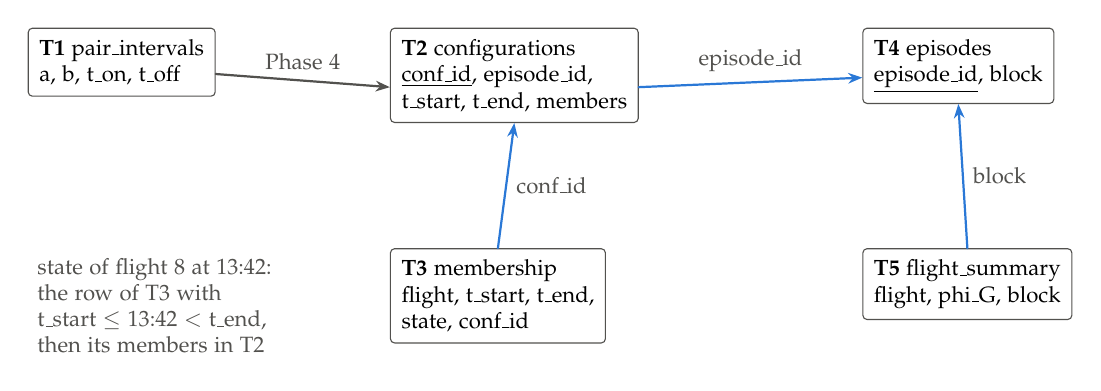
\begin{tikzpicture}[x=1cm,y=1cm,
    tbl/.style={draw=ink2, fill=white, rounded corners=1.5pt, align=left, font=\footnotesize, inner sep=4pt, anchor=north west},
    key/.style={->, blueI, line width=0.8pt}]
  \node[tbl] (t1) at (0,3.6) {\textbf{T1} pair\_intervals\\ a, b, t\_on, t\_off};
  \node[tbl] (t2) at (4.6,3.6) {\textbf{T2} configurations\\ \underline{conf\_id}, episode\_id,\\ t\_start, t\_end, members};
  \node[tbl] (t3) at (4.6,0.8) {\textbf{T3} membership\\ flight, t\_start, t\_end,\\ state, conf\_id};
  \node[tbl] (t4) at (10.6,3.6) {\textbf{T4} episodes\\ \underline{episode\_id}, block};
  \node[tbl] (t5) at (10.6,0.8) {\textbf{T5} flight\_summary\\ flight, phi\_G, block};
  \draw[->, ink2, line width=0.8pt] (t1.east) ++(0,-0.15) -- node[above, note] {Phase 4} ($(t2.west)+(0,-0.15)$);
  \draw[key] (t3.north) -- node[right, note] {conf\_id} (t2.south);
  \draw[key] (t2.east) ++(0,-0.15) -- node[above, note] {episode\_id} ($(t4.west)+(0,-0.15)$);
  \draw[key] (t5.north) -- node[right, note] {block} (t4.south);
  \node[note, anchor=north west, align=left] at (0,0.8) {state of flight 8 at 13:42:\\the row of T3 with\\t\_start $\le$ 13:42 $<$ t\_end,\\then its members in T2};
\end{tikzpicture}
\caption{How the tables connect. Arrows point from a column to the table where it is a key. The
example reads the state of a flight at one instant with an as-of join on T3.}
\label{fig:tables}
\end{figure}

\appendix
\section{Why \texorpdfstring{$m_{ij}(t)=1$ does not give $m_{ji}(t)=1$}{m\_ij(t)=1 does not give m\_ji(t)=1}}\label{app:asymmetry}

$m_{ij}(t)$ of Definition~\ref{def:contact} asks whether $i$, at instant $t$, is at a place that
$j$ visits within $\delta$; $m_{ji}(t)$ asks whether $j$, at the same instant, is at a place that
$i$ visits within $\delta$. These are two questions about two different pairs of instants. Both
are read from one set of correspondences $\M_{ij}$, one on each axis, and they agree only if
that set is symmetric about the diagonal $t'=t$. What does hold:
\begin{itemize}
  \item if $m_{ij}(t)=1$ through the pair $(t,t')$, then $m_{ji}(t')=1$: the same pair, read on
        the other axis, $l=t'-t$ later;
  \item every instant of one indicator lies within $\delta$ of an instant of the other;
  \item the contact $a_{ij}=m_{ij}\vee m_{ji}$ is symmetric: $a_{ij}=a_{ji}$.
\end{itemize}
This appendix keeps only the horizontal condition of $\M_{ij}$: the vertical and heading
conditions only remove pairs. $m_{ij}$ fixes the instant of $i$ and lets that of $j$ vary within
$\pm\delta$; $m_{ji}$ fixes the instant of $j$ and lets that of $i$ vary. Nothing makes the two
answers equal.

\subsection{A worked example}

Take $\delta=120$~s and $\varepsilon_h=500$~m, and ignore heights and headings. Pilot $i$ circles
in a thermal at the point $P$ from 0 to 600~s; the radius of the circle is negligible against
$\varepsilon_h$. Pilot $j$ flies east in a straight line at 10~m/s and is in $P$ at 500~s.

\begin{figure}[htbp]
\centering
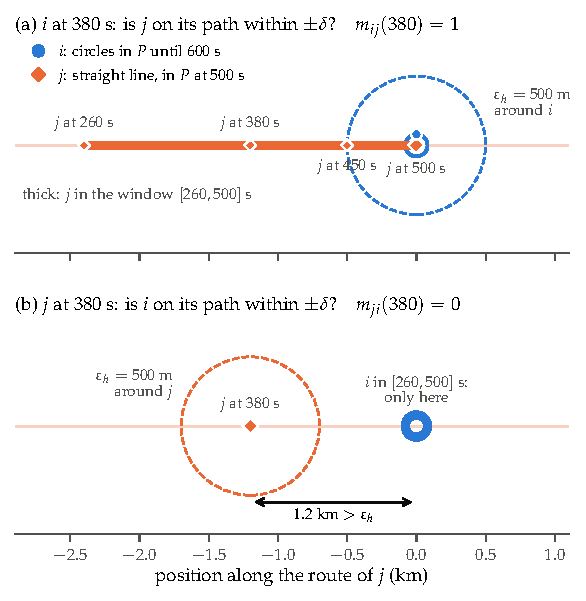
\includegraphics[width=0.74\textwidth]{figures/asymmetry_paths.pdf}
\caption{The example at 380~s. (a)~$i$ is in $P$ and $j$ is 1.2~km west of it. In the window
$[260,500]$~s of $\pm\delta$ (thick), $j$ comes within $\varepsilon_h$ of $i$ at 451~s and is in $P$
at 500~s: the pair $(380,500)$ is a correspondence, so $m_{ij}(380)=1$. (b)~At the same instant
$j$ is 1.2~km from $P$, and during its window $i$ has been only in $P$: no position of $i$ lies
within $\varepsilon_h$ of $j$, so $m_{ji}(380)=0$. The ring only marks $P$.}
\label{fig:asym-paths}
\end{figure}

\begin{table}[htbp]
\centering\small
\begin{tabular}{@{}r l c c c l@{}}
\toprule
$t$ (s) & $j$ relative to $P$ & $m_{ij}$ & $m_{ji}$ & $a_{ij}$ & what happens \\
\midrule
300 & 2.0 km west & 0 & 0 & 0 & $j$ needs more than 120~s to come within 500~m of $P$ \\
380 & 1.2 km west & 1 & 0 & 1 & $i$ is where $j$ will be 120~s later; $j$ is not yet where $i$ has been \\
500 & in $P$ & 1 & 1 & 1 & both are in $P$ \\
560 & 0.6 km east & 1 & 0 & 1 & $i$ is where $j$ was 60~s earlier; $j$ has left \\
\bottomrule
\end{tabular}
\caption{The four instants of the example. Over the whole flight $m_{ij}=1$ from 331 to 600~s,
$m_{ji}=1$ from 451 to 549~s, and $a_{ij}=1$ from 331 to 600~s (strict inequality: exactly
500~m does not count).}
\label{tab:asym-instants}
\end{table}

\subsection{The same example in the plane \texorpdfstring{$(t,t')$}{(t,t')}}

Plot every correspondence $(t,t')$ with the instant at which $i$ passes across and the one at
which $j$ passes up (Figure~\ref{fig:asym-plane}a). Then $m_{ij}(t)=1$ exactly when the
\emph{vertical} line at $t$ meets $\M_{ij}$, and $m_{ji}(t)=1$ exactly when the
\emph{horizontal} line at height $t$ meets it. The two indicators are the shadows of $\M_{ij}$
on the two axes.

At $t=380$ the vertical line meets $\M_{ij}$ (at the pair $(380,500)$ and the ones just below it),
and the horizontal line does not: $\M_{ij}$ has no point with $t'<451$. The set is not symmetric
about the diagonal. The mirror of the pair $(380,500)$ would be $(500,380)$, which needs $i$ at
500~s within 500~m of $j$ at 380~s, and that is 1.2~km away.

\begin{figure}[htbp]
\centering
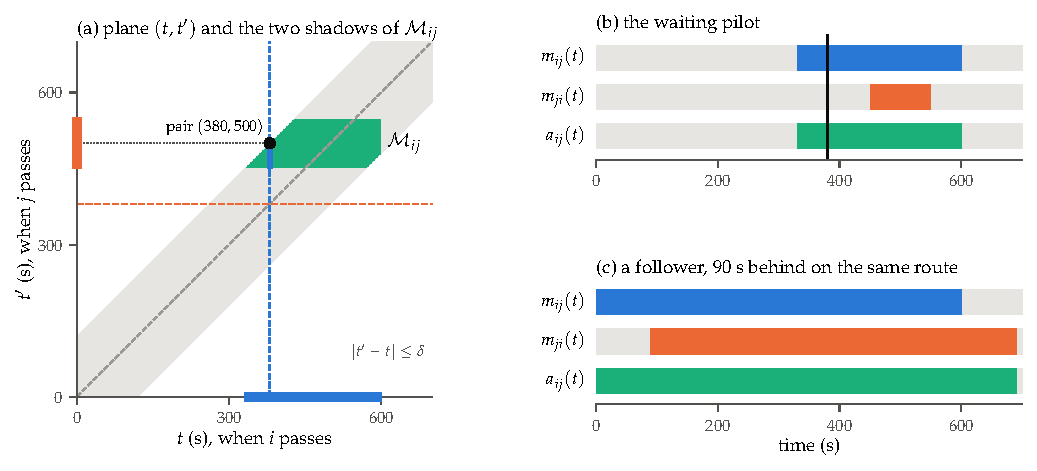
\includegraphics[width=0.94\textwidth]{figures/asymmetry_plane.pdf}
\caption{(a)~The correspondences $\M_{ij}$ (green) in the band $|t'-t|\le\delta$, and its
shadows $m_{ij}$ (blue bar on the $t$ axis) and $m_{ji}$ (orange bar on the $t'$ axis). The
vertical line at 380~s meets $\M_{ij}$ (thick segment), the horizontal one does not. (b)~The
indicators over time, with the line at 380~s. (c)~A pilot $j$ on the same route 90~s behind
$i$: $m_{ji}$ is $m_{ij}$ delayed by exactly 90~s.}
\label{fig:asym-plane}
\end{figure}

\subsection{How far apart they can be}

\textbf{Claim.} If $m_{ij}(t)=1$ there is an instant $t'$ with $|t'-t|\le\delta$ and $m_{ji}(t')=1$;
and conversely.

\emph{Proof.} Take the pair $(t,t')\in\M_{ij}$ that gives $m_{ij}(t)=1$. Then $|t'-t|\le\delta$ by
the definition of $\M_{ij}$, and $m_{ji}(t')=1$ by the definition of $m_{ji}$. The converse is the
same argument read the other way. \hfill$\square$

So the two indicators can differ only by a shift of at most $\delta$. The bound is reached in the
example: the first instant of $m_{ij}$ (331~s) is exactly $\delta$ before the first instant of
$m_{ji}$ (451~s). The union $a_{ij}$ inherits it: at each end of a contact it extends the shorter
indicator by up to $\delta$.

\subsection{Why the contact is the union}

\begin{table}[htbp]
\centering\footnotesize
\begin{tabular}{@{}l c l l@{}}
\toprule
definition & symmetric & in the example & remark \\
\midrule
$m_{ij}\vee m_{ji}$ (used) & yes & 331--600 s & counts the approach and the departure within $\delta$ \\
$m_{ij}\wedge m_{ji}$ & yes & 451--549 s & shorter: each on the path of the other at once \\
$m_{ij}$ alone & no & 331--600 s, or 451--549 s for $(j,i)$ & depends on which pilot is called $i$ \\
\bottomrule
\end{tabular}
\caption{Three ways to define the contact of a pair.}
\label{tab:asym-union}
\end{table}

The union makes the contact independent of the order of the two pilots and keeps the approach and
the departure, where one of them is already on the path of the other. The price is that a contact
starts up to $\delta$ before the pilots are close at the same time. The mutual version
$m_{ij}\wedge m_{ji}$ would give shorter contacts: the false discovery rate and $\tau^*$ would have
to be computed again with the null model, which is not done here.

\textbf{In the code.} \texttt{contacts.scan} returns the instants of $m_{ij}=1$ and, separately,
those of $m_{ji}=1$; \texttt{contacts.pair\_\allowbreak intervals} takes their union. Scenarios:
\texttt{models.WAIT}, \texttt{models.FOLLOW}; figures: \texttt{plots.asymmetry}; numbers checked
in \texttt{test\_note.py}.

\section{Graphs, from scratch}\label{app:graphs}

The few terms of graph theory that the note uses, each with the place where it is used. The terms
of the study of the groups, shape and order of a group and the configuration model, are in
the note \emph{The structure of groups in free flight}.

\begin{itemize}
  \item \textbf{Graph.} A set of \emph{nodes} and a set of \emph{edges}, each edge joining two
        nodes. The active graph $G(t)$ of Section~\ref{sec:configurations} has a node for each flight
        and an edge for each pair interval in progress.
  \item \textbf{Path.} A sequence of nodes, each joined by an edge to the next. Two nodes are
        \emph{connected} when a path joins them.
  \item \textbf{Connected component.} A largest set of nodes connected to each other. Every node is
        in exactly one component; a node with no edge is a component alone (a pilot flying solo).
        A configuration is a component with at least two nodes, with its edges.
\end{itemize}

Two members of a configuration need not share an edge: in the chain 1--2--3 of
Figure~\ref{fig:graph}, pilots 1 and 3 are in the same configuration through pilot 2.

\begin{figure}
\centering
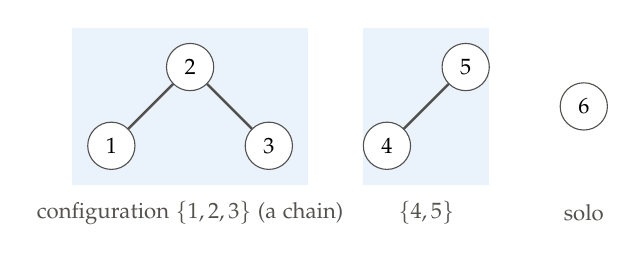
\begin{tikzpicture}[x=1cm,y=1cm, node/.style={circle, draw=ink2, fill=white, minimum size=6mm, inner sep=0pt,
    font=\footnotesize}, gedge/.style={ink2, line width=0.9pt}]
  \fill[blueI!10] (-0.5,-0.5) rectangle (2.5,1.5);
  \fill[blueI!10] (3.2,-0.5) rectangle (4.8,1.5);
  \node[node] (a) at (0,0) {1}; \node[node] (b) at (1,1) {2}; \node[node] (c) at (2,0) {3};
  \node[node] (d) at (3.5,0) {4}; \node[node] (e) at (4.5,1) {5}; \node[node] (f) at (6,0.5) {6};
  \draw[gedge] (a) -- (b) -- (c); \draw[gedge] (d) -- (e);
  \node[note] at (1,-0.85) {configuration $\{1,2,3\}$ (a chain)};
  \node[note] at (4,-0.85) {$\{4,5\}$};
  \node[note] at (6,-0.85) {solo};
\end{tikzpicture}
\caption{The graph at one instant: three components, two of them configurations.}
\label{fig:graph}
\end{figure}

\begin{itemize}
  \item \textbf{Directed graph.} The edges carry an arrow. For the episodes the nodes are
        groups, with an arrow $g\to g'$ when $g'$ starts as $g$ ends and they share a member
        (Section~\ref{sec:episodes}). An episode is a connected component of this graph, arrows
        ignored.
  \item \textbf{Bipartite graph.} Nodes of two kinds, edges only between kinds. At one instant, the
        groups ending and those starting, with an edge when they share a member. Each
        component is one event (Figure~\ref{fig:events}); its outcome follows from how many
        groups it has on each side: one to one is a join or a leave (members added or
        removed), one to several a split, several to one a merge (Section~\ref{gs-sec:describe} of the note on the structure of groups).
\end{itemize}

\begin{figure}
\centering
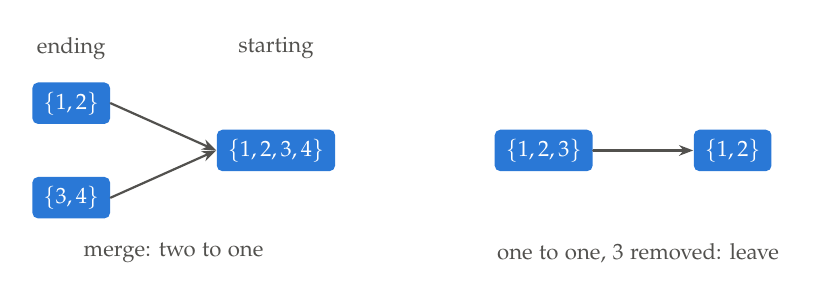
\begin{tikzpicture}[x=1cm,y=1cm, conf/.style={rounded corners=2pt, fill=blueI, text=white, font=\footnotesize,
    minimum height=5mm, inner xsep=4pt}, link/.style={->, ink2, line width=0.8pt}]
  \node[conf] (c1) at (0,0.6) {$\{1,2\}$}; \node[conf] (c2) at (0,-0.6) {$\{3,4\}$};
  \node[conf] (c3) at (2.6,0) {$\{1,2,3,4\}$};
  \draw[link] (c1.east) -- (c3.west); \draw[link] (c2.east) -- (c3.west);
  \node[note] at (1.3,-1.3) {merge: two to one};
  \node[conf] (d1) at (6,0) {$\{1,2,3\}$};
  \node[conf] (d2) at (8.4,0) {$\{1,2\}$};
  \draw[link] (d1.east) -- (d2.west);
  \node[note] at (7.2,-1.3) {one to one, 3 removed: leave};
  \node[note] at (0,1.3) {ending}; \node[note] at (2.6,1.3) {starting};
\end{tikzpicture}
\caption{Two events: each is a connected component of the bipartite graph of the groups
ending and starting at one instant.}
\label{fig:events}
\end{figure}

\section{Two models}\label{app:models}

\paragraph{Ornstein--Uhlenbeck process}~\cite{uhlenbeck1930} (Section~\ref{sec:cohesion}). A quantity
$\ell$ pulled back to 0 by a spring of rate $k$ and shaken by noise:
\begin{equation}
  d\ell=-k\,\ell\,dt+\sqrt{2k}\,\sigma\,dW .
\end{equation}
It forgets its value after $1/k$ and spreads by $\sigma$ around 0. Its mean square change after a
lag $s$ is $D(s)=\langle(\ell(t+s)-\ell(t))^2\rangle=2\sigma^2(1-e^{-ks})$: it grows as
$2k\sigma^2 s$ at short lags, like a free random walk, and stops at $2\sigma^2$ after $1/k$. With
$k=0$ it is a random walk and $D$ grows forever. A measurement noise of variance $c/2$ on each
value adds $c$ to $D(s)$ at every lag.

\paragraph{Birth--death chain} (Section~\ref{sec:fission}). A group of $n$ pilots gains one at rate
$g(n)$ and loses one at rate $l(n)$. Over a long time the transitions from $n$ to $n+1$ and back are
equally many, so the time spent at $n+1$ and at $n$, $T(n+1)$ and $T(n)$, satisfy
$T(n)\,g(n)=T(n+1)\,l(n+1)$, Eq.~\eqref{eq:chain}. Multiplying the ratios from 2 to $n$ gives
$T(n)$. If every member joins others at rate $a$ and leaves at rate $\mu$, $g(n)=an$, $l(n)=\mu n$
and $T(n)\propto x^n/n$ with $x=a/\mu$, the log-series: the tail falls exponentially. A leaving rate
that falls with $n$ makes it heavier.

\section{Further evidence}\label{app:evidence}

These measurements support Sections~\ref{sec:calibration} and~\ref{sec:tuning} without changing
their conclusions.

\paragraph{The time shifts of the surrogates} (Section~\ref{sec:null}). Figure~\ref{fig:shifts}
gives the whole distribution behind the median of 58~min.

\begin{figure}
\centering
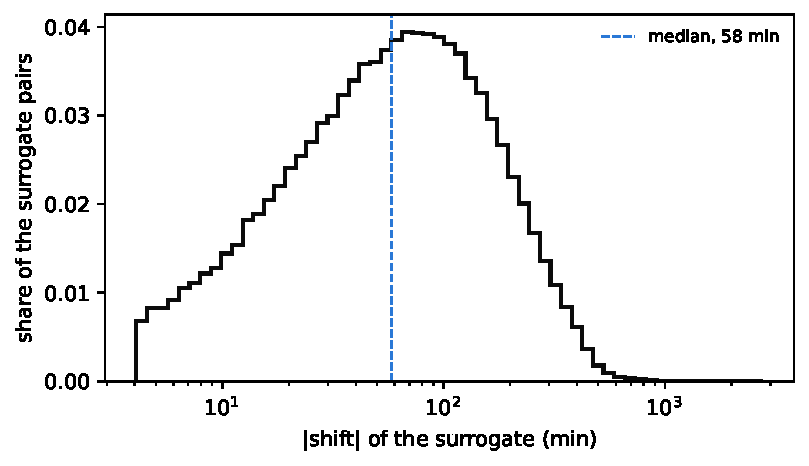
\includegraphics[width=0.62\textwidth]{figures/assessment_shifts.pdf}
\caption{The time shifts $|r_{ij}|$ of the 248\,741 surrogate pairs of the chosen run, whole
archive.}
\label{fig:shifts}
\end{figure}

\paragraph{The delay inside the contacts} (Section~\ref{sec:delta-choice}). Figure~\ref{fig:ell}
gives the whole distribution behind Table~\ref{tab:ell}: short intervals spread over the window
and pile up at its edge, long ones gather at small delays.

\begin{figure}
\centering
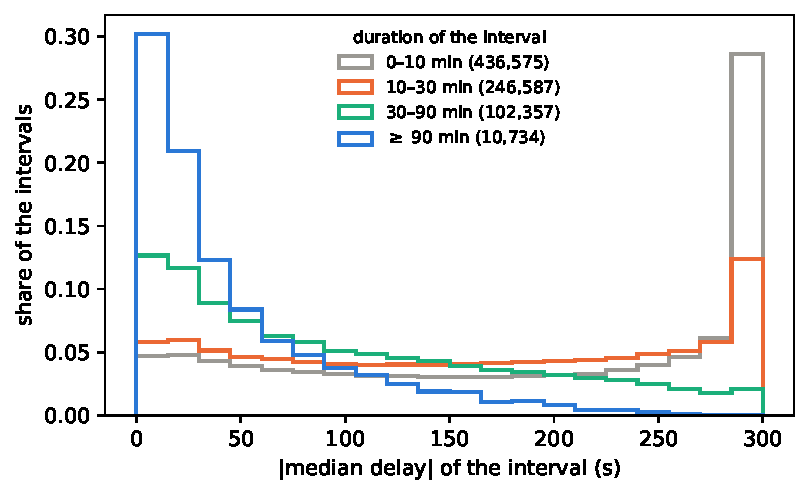
\includegraphics[width=0.62\textwidth]{figures/assessment_ell.pdf}
\caption{Distribution of the $|\ell_{\rm med}|$ of the pair intervals, by their duration
($\delta=5$~min, whole archive).}
\label{fig:ell}
\end{figure}

\paragraph{The distance at the same instant} (Section~\ref{sec:delta-choice}). Is there a distance
beyond which two pilots stop being closer than chance? We counted the distance between the two
pilots at every grid instant when both fly after departure, without requiring a correspondence,
for all the real pairs and for the surrogates, on the dates of Figure~\ref{fig:delays} that have
surrogates (210 of 300, 58\,901~h of real exposure). Real pairs are much closer than chance at
short distance and have no edge (Figure~\ref{fig:separation}): the ratio $g(d)$ is 10.4 within
100~m, below 2 from 500~m, below 1.5 from 900~m, below 1.1 from 2.7~km and below 1 from 5.7~km.
Real pairs spend 6.6\% of their time together within 1~km of each other, against 2.8\% by chance.
Beyond 6~km $g$ falls slightly below 1, because both distributions sum to one.

The excess reaches several kilometres, beyond the visual range of 1.5~km of
Section~\ref{sec:delta}. Since the surrogates also change the hour, this excess may hold the
weather of the hour as well as sight, so it bounds neither the visual range nor the range of
following.

\begin{figure}
\centering
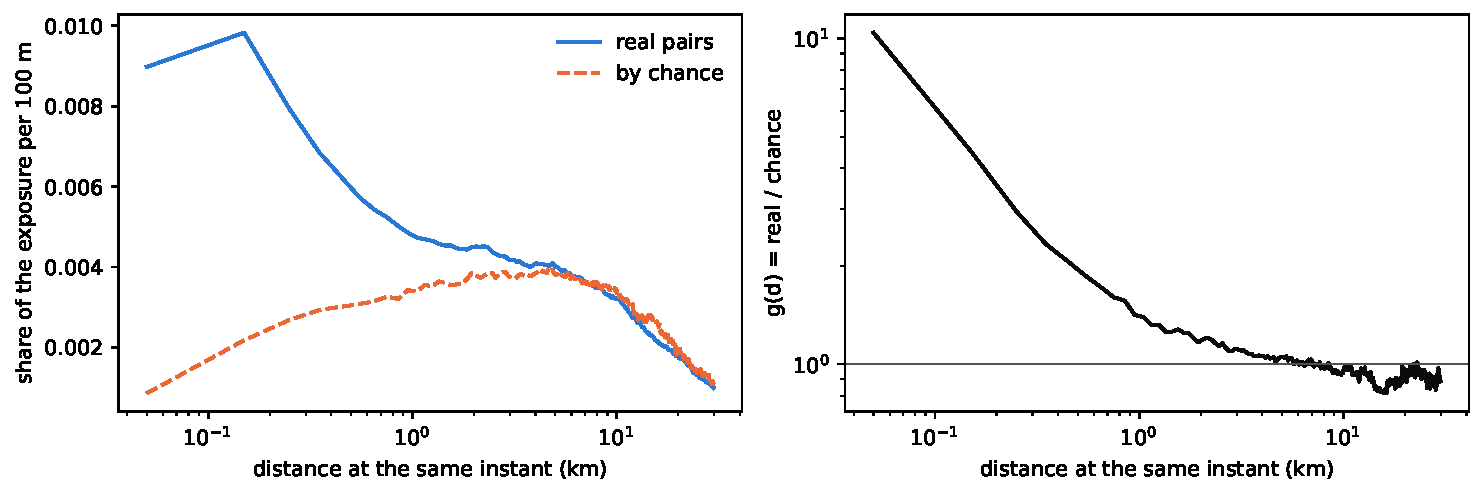
\includegraphics[width=\textwidth]{figures/assessment_separation.pdf}
\caption{Distance between the two pilots at the same instant, over all the time both fly, on
210 dates. Left: share of the exposure in each 100~m bin, real pairs and chance. Right: their
ratio $g(d)$.}
\label{fig:separation}
\end{figure}

\paragraph{One parameter at a time} (Section~\ref{sec:plateau}). Table~\ref{tab:plateau}.

\begin{table}
\centering
\small
\begin{tabular}{@{}l c c c c@{}}
\toprule
Setting ($\delta=5$ min unless stated) & $\tau^*$ (min) & $f_G$ & episodes & flights in a group \\
\midrule
starting values & 126.1 & 0.034 & 98 & 210 \\
$\varepsilon_h=250$ m & 75.1 & 0.058 & 253 & 537 \\
$\varepsilon_h=1000$ m & 126.8 & 0.065 & 162 & 372 \\
$\varepsilon_z=150$ m & 126.1 & 0.020 & 61 & 125 \\
$\varepsilon_z=600$ m & 126.1 & 0.044 & 122 & 268 \\
$\delta=2$ min & 42.6 & 0.106 & 600 & 1\,170 \\
$\delta=10$ min & 128.4 & 0.062 & 153 & 365 \\
$\theta_{\max}=30^\circ$ & 126.1 & 0.034 & 97 & 208 \\
$\theta_{\max}=90^\circ$ & 126.1 & 0.034 & 98 & 210 \\
$g=60$ s & 75.8 & 0.087 & 332 & 732 \\
$g=300$ s & 126.1 & 0.055 & 141 & 318 \\
\bottomrule
\end{tabular}
\caption{One parameter at a time on 300 random dates (7\,051 flights), $q=0.05$.}
\label{tab:plateau}
\end{table}

\begin{thebibliography}{28}
\small

\bibitem{akos2008} Z. Ákos, M. Nagy, T. Vicsek. Comparing bird and human soaring strategies.
\emph{Proceedings of the National Academy of Sciences} 105(11):4139--4143, 2008.

\bibitem{amornbunchornvej2018a} C. Amornbunchornvej, I. Brugere, A. Strandburg-Peshkin, D. R. Farine,
M. C. Crofoot, T. Y. Berger-Wolf. Coordination event detection and initiator identification in time
series data. \emph{ACM Transactions on Knowledge Discovery from Data} 12(5), 2018.
doi:10.1145/3201406.

\bibitem{amornbunchornvej2018b} C. Amornbunchornvej, T. Y. Berger-Wolf. Framework for inferring
leadership dynamics of complex movement from time series. \emph{Proceedings of the SIAM
International Conference on Data Mining}, 549--557, 2018.

\bibitem{amornbunchornvej2021} C. Amornbunchornvej. mFLICA: an R package for inferring leadership of
coordination from time series. \emph{SoftwareX}, 2021. doi:10.1016/j.softx.2021.100781. Preprint
arXiv:2004.06092.

\bibitem{andersson2007} M. Andersson, J. Gudmundsson, P. Laube, T. Wolle. Reporting leadership
patterns among trajectories. \emph{Proceedings of the ACM Symposium on Applied Computing}, 3--7,
2007.

\bibitem{bonabeau1999} E. Bonabeau, L. Dagorn, P. Fréon. Scaling in animal group-size distributions.
\emph{Proceedings of the National Academy of Sciences} 96:4472--4477, 1999.

\bibitem{buchin2015} K. Buchin, M. Buchin, M. van Kreveld, B. Speckmann, F. Staals. Trajectory
grouping structure. \emph{Journal of Computational Geometry} 6(1), 2015.
doi:10.20382/jocg.v6i1a3. Preliminary version: WADS 2013; arXiv:1303.6127.

\bibitem{chen2005} L. Chen, M. T. Özsu, V. Oria. Robust and fast similarity search for moving
object trajectories. \emph{Proceedings of ACM SIGMOD}, 491--502, 2005.

\bibitem{flack2018} A. Flack, M. Nagy, W. Fiedler, I. D. Couzin, M. Wikelski. From local collective
behavior to global migratory patterns in white storks. \emph{Science} 360(6391):911--914, 2018.

\bibitem{greene2010} D. Greene, D. Doyle, P. Cunningham. Tracking the evolution of communities in
dynamic social networks. \emph{Proceedings of the International Conference on Advances in Social
Networks Analysis and Mining (ASONAM)}, 176--183, 2010.

\bibitem{gudmundsson2006} J. Gudmundsson, M. van Kreveld. Computing longest duration flocks in
trajectory data. \emph{Proceedings of ACM GIS}, 2006.

\bibitem{jeung2008} H. Jeung, M. L. Yiu, X. Zhou, C. S. Jensen, H. T. Shen. Discovery of convoys in
trajectory databases. \emph{Proceedings of the VLDB Endowment} 1(1), 2008.

\bibitem{joo2018} R. Joo, M.-P. Etienne, N. Bez, S. Mahévas. Metrics for describing dyadic movement:
a review. \emph{Movement Ecology} 6:26, 2018.

\bibitem{konzack2017} M. Konzack, T. McKetterick, T. Ophelders, M. Buchin, L. Giuggioli, J. Long,
T. Nelson, M. A. Westenberg, K. Buchin. Visual analytics of delays and interaction in movement
data. \emph{International Journal of Geographical Information Science} 31(2):320--345, 2017.

\bibitem{li2010} Z. Li, B. Ding, J. Han, R. Kays. Swarm: mining relaxed temporal moving object
clusters. \emph{Proceedings of the VLDB Endowment} 3(1), 2010.

\bibitem{li2013} Z. Li, F. Wu, M. C. Crofoot. Mining following relationships in movement data.
\emph{Proceedings of the 13th IEEE International Conference on Data Mining (ICDM)}, 458--467, 2013.
doi:10.1109/ICDM.2013.98.

\bibitem{long2014} J. A. Long, T. A. Nelson, S. L. Webb, K. L. Gee. A critical examination of indices
of dynamic interaction for wildlife telemetry studies. \emph{Journal of Animal Ecology}
83(5):1216--1233, 2014.

\bibitem{long2022} J. A. Long, S. L. Webb, S. M. Harju, K. L. Gee. Analyzing contacts and behavior
from high frequency tracking data using the wildlifeDI R package. \emph{Geographical Analysis}
54:648--663, 2022.

\bibitem{nagy2010} M. Nagy, Z. Ákos, D. Biro, T. Vicsek. Hierarchical group dynamics in pigeon
flocks. \emph{Nature} 464:890--893, 2010.

\bibitem{nagy2018} M. Nagy, I. D. Couzin, W. Fiedler, M. Wikelski, A. Flack. Synchronization,
coordination and collective sensing during thermalling flight of freely migrating white storks.
\emph{Philosophical Transactions of the Royal Society B} 373:20170011, 2018.

\bibitem{newman2010} M. E. J. Newman. \emph{Networks: An Introduction}. Oxford University Press,
2010.

\bibitem{ruzzo1999} W. L. Ruzzo, M. Tompa. A linear time algorithm for finding all maximal scoring
subsequences. \emph{Proceedings of ISMB}, 1999.

\bibitem{sakoe1978} H. Sakoe, S. Chiba. Dynamic programming algorithm optimization for spoken word
recognition. \emph{IEEE Transactions on Acoustics, Speech, and Signal Processing} 26(1):43--49,
1978.

\bibitem{spiegel2016} O. Spiegel, S. T. Leu, A. Sih, C. M. Bull. Socially interacting or indifferent
neighbours? Randomization of movement paths to tease apart social preference and spatial
constraints. \emph{Methods in Ecology and Evolution} 7(8):971--979, 2016.

\bibitem{su2020} H. Su, S. Liu, B. Zheng, X. Zhou, K. Zheng. A survey of trajectory distance
measures and performance evaluation. \emph{The VLDB Journal} 29:3--32, 2020.

\bibitem{tarjan1975} R. E. Tarjan. Efficiency of a good but not linear set union algorithm.
\emph{Journal of the ACM} 22(2):215--225, 1975.

\bibitem{virtanen2020} P. Virtanen et al. SciPy 1.0: fundamental algorithms for scientific
computing in Python. \emph{Nature Methods} 17:261--272, 2020.

\bibitem{tusher2001} V. G. Tusher, R. Tibshirani, G. Chu. Significance analysis of microarrays applied
to the ionizing radiation response. \emph{Proceedings of the National Academy of Sciences}
98(9):5116--5121, 2001.

\bibitem{uhlenbeck1930} G. E. Uhlenbeck, L. S. Ornstein. On the theory of the Brownian motion.
\emph{Physical Review} 36:823--841, 1930.

\bibitem{vlachos2002} M. Vlachos, G. Kollios, D. Gunopulos. Discovering similar multidimensional
trajectories. \emph{Proceedings of the 18th International Conference on Data Engineering (ICDE)},
2002.

\bibitem{williams2018} H. J. Williams, A. J. King, O. Duriez, L. Börger, E. L. C. Shepard. Social
eavesdropping allows for a more risky gliding strategy by thermal-soaring birds. \emph{Journal of
the Royal Society Interface} 15:20180578, 2018.

\end{thebibliography}


\end{document}
